%start of chapter till prob 5.5
%==================
\باب{متماثل ذرات}\شناخت{باب_متماثل_ذرات}
\حصہ{دو    ذراتی نظام} 
ایک ذروی کے لیے ( فی الحال چکر کو نظر انداز کرتے ہوئے )     \عددی{ \psi ( \kvec{r} , t )}  فضا ٗی محدد، \عددی{ \kvec{r}}،  اور وقت،  \عددی{ t}،  کا تفاعل ہو گا۔ دو ذراتی نظام کا حال پہلے ذرے کے محدد ، \عددی{ ( \kvec{r}_1 ) }،  دوسرے ذرے کے محدد ، \عددی{ ( \kvec{r}_2 ) }،  اور وقت کا تابع ہو گا۔ 
\begin{align}   
\psi ( \kvec{r}_1 , \kvec{r}_2 , t ) 
\end{align}
 ہمیشہ کی طرح یہ وقت کے لحاظ سے شروڈنگر مساوات 
\begin{align}
i \hslash \frac{ \partial \psi }{ \partial t } = H \psi
\end{align}
کے تحت ارتقا کرے گا جہاں \عددی{ H} مکمل  نظام کا ہیملٹنی  ہے۔
\begin{equation}
H = - \frac{ \hslash^2 }{ 2 m_1 } \nabla_1^2  -  \frac{ \hslash^2 }{ 2 m_2 }  \nabla_2^2 +  V(\kvec{r}_1 , \kvec{r}_2 , t )
\end{equation}
ذرہ  \عددی{1}  اور  ذرہ  \عددی{2}   کے محدد کے لحاظ سے  تفرقات  کو  \عددی{\nabla} کے  زیر نوشت میں بالترتیب  \عددی{1}  اور    \عددی{2}  سے ظاہر کیا گیا ہے۔ ذرہ  \عددی{1}  کا
 حجم  \عددی{ \dif^{\,3} \kvec{r}_1 } اور ذرہ  \عددی{2}  کا حجم \عددی{ \dif^{\,3} \kvec{r}_2} میں  پائے جانے کا احتمال درج ذیل ہو گا:
\begin{align}
\abs{\psi (\kvec{r}_1 , \kvec{r}_2 , t ) }^2  {\dif^{\,3} } { \kvec{r}_1 }  {\dif^{\,3} } { \kvec{r}_2 }
\end{align}
جہاں شماریاتی مفہوم   معمول کے مطابق کارآمد ہو گا۔ ظاہر ہے کہ  \عددی{ \psi} کو درج ذیل کے تحت  معمول پر لانا ہو گا۔ 
\begin{align}
\int \abs{\psi ( \kvec{r}_1 , \kvec{r}_2 , t ) }^2 {\dif^{\,3} } {\kvec{r}_1 } {\dif^{\,3} } { \kvec{r}_2 } = 1
\end{align}

غیر تابع وقت مخفیہ کے لیے علیحدگی  متغیرات  سے حلوں کا   مکمل سلسلہ :
\begin{align}
\psi ( \kvec{r}_1 , \kvec{r}_2 , t ) =  \psi ( \kvec{r}_1 , \kvec{r}_2 ) {e}^{-i E t/\hslash}  
\end{align}
حاصل ہو گا جہاں فضا ٗی تفاعل موج  \عددی{( \psi)} غیر تابع وقت شروڈنگر مساوات :
\begin{align}
-\frac{ \hslash }{ 2 m_1 }  {\nabla_1^2} { \psi } - \frac{ \hslash }{ 2 m_2 } \nabla_2^2 { \psi } + V \psi =E\psi
\end{align}
کو مطمئن کرتا ہے جس میں \عددی{E}   نظام کی کل توانائی ہے ۔ 

\ابتدا{سوال}\شناخت{سوال_متماثل_تخفیف_شدہ_کمیت}
عام طور پر  باہم عمل  مخفیہ  کا  انحصار صرف دو  ذرات کے بیچ سمتیہ \عددی{ \kvec{r} = \kvec{r}_1 - \kvec{r}_2 } پر ہو گا ۔ ایسی صورت میں متغیرات  \عددی{ \kvec{r}_1} اور  \عددی{  \kvec{r}_2} کی جگہ نئے  متغیرات \عددی{\kvec{r}}   اور
( مرکز کمیت)  \عددی{  \kvec{R} \equiv\frac{ ( m_1 \kvec{r}_1 + m_2 \kvec{r}_2 ) }{ m_1 + m_2 }}کے  استعمال سے  مساوات شروڈنگر دو  حصوں  میں علیحدہ ہو گی ۔  
\begin{enumerate}[a.]
\item
درج ذیل   دکھائیں
\begin{align*}
 \kvec{r}_1 &= \kvec{R} + \tfrac{ \mu}{m_1}\kvec{r}, && \kvec{r}_2 = \kvec{R} - \tfrac{ \mu }{ m_2 } \kvec{r}\\
  \nabla_1& = \tfrac{ \mu }{ m_2 }\nabla_R + \nabla_r , &&  \nabla_2 = \tfrac{ \mu }{ m_1 } \nabla_R - \nabla_r
\end{align*}
جہاں 
\begin{align}\label{مساوات_متماثل_تخفیف_شدہ_کمیت}
\mu = \frac{ m_1 m_2 }{ m_1 + m_2 }
\end{align}
نظام کی  \اصطلاح{تخفیف شدہ کمیت}\فرہنگ{کمیت!تخفیف شدہ}\حاشیہب{reduced mass}\فرہنگ{mass!reduced} ہے ۔
\item 
  دکھائیں کہ (غیر تابع وقت)  شروڈنگر  مساوات درج ذیل روپ اختیار کرتی ہے ۔
\begin{align*}
- \frac{ \hslash^2 }{ 2 ( m_1 + m_2 ) } \nabla_R^2  \psi - \frac{ \hslash^2 }{ 2 \mu }\nabla_r^2 { \psi } + V(\kvec{r}) \psi = E \psi
\end{align*}
\item
 متغیرات کو  \عددی{ \psi (\kvec{R} ,\kvec{r} ) = { \psi_R }(\kvec{R}) { \psi_r } (\kvec{r}) } لیتے ہوئے علیحدہ کریں ۔ آپ دیکھیں گے کہ  \عددی{ \psi_R }  یک ذروی  شروڈنگر مساوات، جس میں کمیت \عددی{m} کی بجائے  کل کمیت  \عددی{ ( m_1 + m_2 ) }، مخفیہ  صفر ہو اور نظام کی توانائی  \عددی{ E_R } ہو،   کو مطمئن کرتا ہے  جبکہ  \عددی{ \psi_r } یک ذروی  شروڈنگر مساوات، جس میں کمیت \عددی{m} کی بجائے  تخفیف شدہ کمیت، مخفیہ  \عددی{  V(\kvec{r})}  اور توانائی \عددی{E_r} ہو، کو مطمئن کرتا ہے ۔ کل توانائی  ان کا مجموعہ:   \عددی{ E = E_R + E_r } ہو گا ۔ اس سے ہمیں یہ معلوم ہوتا ہے  کہ مرکز  کمیت ایک آزاد ذرہ کی مانند  حرکت کرتا ہے اور(  ذرہ  \عددی{1} کے لحاظ سے ذرہ  \عددی{2}  کی)  \ترچھا{ نسبتی} حرکت ایسی  ہو گی جیسا مخفیہ \عددی{ V} میں تخفیف شدہ کمیت کا ایک ذروی  کرتا ہے۔ کلاسیکی میکانیات میں  بالکل یہی تحلیل ہو گی    جو دو  جسمی  مسئلہ کو معادل یک جسمی مسئلہ میں  تبدیل کرتی ہے ۔ 
\end{enumerate}
\انتہا{سوال}
\ابتدا{سوال}\شناخت{سوال_متماثل_درستگی}
 یوں ہائیڈروجن کے مرکزہ کی حرکت کو درست کرنے کے لیے ہم الیکٹران  کی کمیت کی جگہ تخفیف شدہ کمیت استعمال کرتے ہیں  (سوال \حوالہ{سوال_متماثل_تخفیف_شدہ_کمیت})۔ 
\begin{enumerate}[a.]
\item
 ہائیڈروجن کی بندشی  توانائی (مساوات \حوالہ{مساوات_تین_ابعاد_ہائیڈروجن_بندشی_توانائی}) جاننے کی خاطر  \عددی{ \mu } کی جگہ m استعمال کرنے سے پیدا فی صد  سہو   دو با معنی ہندسوں تک   تلاش کریں۔  
\item
 ہائیڈروجن اور ڈیوٹریم کے لیے   سرخ بالمر لکیروں   \عددی{(n=3\to n=2)}   کے طول موج کے بیچ    فاصلہ  (فرق)تلاش کریں ۔ 
\item
 \اصطلاح{پازیٹرانیم}\فرہنگ{پازیٹرانیم}\حاشیہب{positronium}\فرہنگ{positronium} کی بندشی توانائی تلاش کریں ۔ پروٹان کی جگہ  ضد الیکٹران رکھنے سے پازیٹرانیم پیدا ہو گا ۔ ضد الیکٹران کی کمیت الیکٹران کی کمیت کے برابر   جبکہ اس کا بار  الیکٹران کے بار  کے مخالف ہے ۔ 
\item
 فرض کریں آپ  \اصطلاح{میونی ہائیڈروجن}\فرہنگ{ہائیڈروجن!میونی}\حاشیہب{muonic hydrogen}\فرہنگ{hydrogen!muonic} (    جس میں الیکٹران کی جگہ ایک میون  ہو گا) کی وجودیت گی کی تصدیق کرنا جانتے ہیں۔ میون کا بار  الیکٹران کے بار  کے برابر ہے ، تاہم  اس کی کمیت  الیکٹران سے\عددی{206.77} گنا زیادہ   ہے ۔  آپ لیمان  \عددی{\alpha}  لکیر   \عددی{n=2\to n=1} کے لیے کس طول  موج پر نظر رکھیں گے ؟
\end{enumerate}
\انتہا{سوال}
\ابتدا{سوال}
کلورین کے قدرتی دو ہم جا   \عددی{\ce{Cl^{35}}} اور \عددی{\ce{Cl^{37}}}   پائے جاتے ہیں ۔ دکھائیں کہ  \عددی{\ce{HCl}} کا   لرزشی   طیف قریب قریب   جوڑیوں پر مشتمل ہو گا   جن میں فاصلہ   \عددی{ \Delta \nu = 7.51 \times {10}^{-4} \nu } ہو گا جہاں \عددی{ \nu} خارجی نوریہ کا تعدد ہے ۔  ( اشارہ : اس کو ایک ہارمونی مرتعش تصور کریں جہاں  \عددی{ \omega = \sqrt{ \frac{ k }{ mu} } } ہو گا   جہاں  \عددی{ \mu } تخفیف شدہ کمیت ( مساوات  \حوالہ{مساوات_متماثل_تخفیف_شدہ_کمیت} ) ہے   جبکہ  دونوں ہم جا  کا   \عددی{ k} ایک دوسرے  جیسا تصور کریں ۔) 
\انتہا{سوال}

%the above is p213-p215
%==============================================

\جزوحصہ{بوزان اور فرمیان}
فرض کریں ذرہ  \عددی{1} (ایک ذروی حال ) \عددی{\psi_a(\kvec{r})} اور ذرہ  \عددی{2}  حال \عددی{\psi_b(\kvec{r})} میں پائے جاتے ہیں۔( یاد رہے،   میں یہاں چکر کو نظرانداز کر رہا ہوں۔)  ایسی صورت میں \عددی{\psi(\kvec{r}_1, \kvec{r}_2)} سادہ حاصل ضرب ہوگا۔\حاشیہد{در حقیقت، ضروری نہیں کہ ہر دو  ذروی   تفاعل موج دو ایک ذروی تفاعلات موج کا حاصل ضرب ہو۔ ایسے حال جنہیں  \اصطلاح{ ہمبستہ  حال}\فرہنگ{ہمبستہ  حال}\تحریر{(entangled states)}\فرہنگ{entangled states} کہتے ہیں کو اس طرح  دو حصوں میں  علیحدہ نہیں کیا جا سکتا ہے۔ تاہم اگر ذرہ \عددی{1} حال \عددی{a} اور ذرہ \عددی{2} حال \عددی{b} میں ہوں، تب دو ذروی  حال حاصل ضرب ہو گا۔ میں جانتا ہوں، آپ سوچ رہے ہیں:"  ذرہ \عددی{1} کیسے کسی حال میں اور ذرہ \عددی{2} کسی دوسرے حال میں نہیں ہوں گے؟" اس کی کلاسیکی مثال یک تا چکری تشاکل ہے (مساوات \حوالہ{مساوات_تین_ابعادی_یک_تا_حال})؛ میں آپ کو  اکیلے ذرہ \عددی{1} کا حال نہیں بتا سکتا ہوں، چونکہ یہ ذرہ \عددی{2} کے حال کے ساتھ  ہمبستہ ہے۔ اگر \عددی{2} کی پیمائش کی جائے اور  نتیجہ  ہم میدان چکر  ہو تب \عددی{1} ہم میدان چکر  اور \عددی{2} مخالف میدان چکر  ہو گا۔}
\begin{align}
	\psi(\kvec{r}_1, \kvec{r}_2)=\psi_a(\kvec{r}_1)\psi_b(\kvec{r}_2)
\end{align}
 ہم یہاں  فرض کر رہے ہیں  ان ذرات کو علیحدہ علیحدہ پہچانا جا  سکتا ہے؛  ورنہ یہ کہنا کہ ذرہ \عددی{1} حال \عددی{\psi_a}  اور ذرہ \عددی{2} حال \عددی{\psi_b} میں ہے بے معنی ہو  گا؛   ہم  صرف اتنا کہہ پاتے کہ ایک ذرہ  حال  \عددی{\psi_a} اور دوسرا ذرہ  حال \عددی{\psi_b} میں پایا جاتا ہے، تاہم ہم نہیں جان پاتے کہ کونسا ذرہ کس حال میں ہے۔ کلاسیکی میکانیات میں یہ ایک بے وقوفانہ  اعتراض ہو گا: اصولاً ایک ذرے کو سرخ رنگ اور دوسرے کو نیلا رنگ دے کر آپ انہیں ہر وقت پہچان سکتے ہیں۔ کوانٹم میکانیات میں صورتحال بنیادی طور پر مختلف ہے:  آپ کسی الیکٹران کو سرخ رنگ نہیں دے سکتے  اور نہ ہی اس پر کوئی پرچی چسپاں کر سکتے ہیں۔ حقیقت یہ ہے کہ تمام الیکٹران بالکل متماثل ہوتے ہیں جبکہ کلاسیکی اشیاء اتنی یکسانیت کبھی نہیں رکھ سکتے ہیں۔ ایسا نہیں ہے کہ ہم الیکٹرانوں کو پہچاننے سے قاصر ہیں بلکہ حقیقت یہ ہے کہ"یہ" الیکٹران اور "وہ"   الیکٹران   کہنا کوانٹم میکانیات میں بے معنی ہیں؛   ہم صرف"ایک" الیکٹران کی بات کر سکتے ہیں۔
 
ایسے    ذرات کی موجودگی کو،  جو \ترچھا{  اصولاً  غیر ممیز} ہوتے ہیں،   کوانٹم میکانیات خوش اسلوبی سے سموتی ہے: ہم  ایسا  \ترچھا{غیر مشروط } تفاعل موج  تیار کرتے ہیں جو یہ بات  نہیں کرتا کہ  کونسا  ذرہ کس  حال میں ہے۔  ایسا   دو (ذیل) طریقوں سے کرنا ممکن ہے۔
\begin{align}\label{مساوات_متماثل_غیر_مشروط_حال}
	\psi_{\pm}(\kvec{r}_1, \kvec{r}_2)=A[\psi_a(\kvec{r}_1)\psi_b(\kvec{r}_2)\pm\psi_b(\kvec{r}_1)\psi_a(\kvec{r}_2)]
\end{align}
یوں یہ  ذرہ دو اقسام کے متماثل ذرات کا حامل ہوگا: \اصطلاح{ بوزان}\فرہنگ{بوزان}\حاشیہب{bosons}\فرہنگ{bosons} جن کے لئے ہم مثبت علامت استعمال کرتے ہیں اور \اصطلاح{فرمیان}\فرہنگ{فرمیان}\حاشیہب{fermions}\فرہنگ{fermions} جن کے لئے ہم منفی علامت استعمال کرتے ہیں۔ بوزان کی مثالیں نوریہ اور میزون ہیں جبکہ فرمیان کی مثالیں  پروٹان اور الیکٹران ہیں۔ ایسا ہے کہ
\begin{align}
\left.	\begin{tabular}{r}
		\ترچھا{عدد صحیح} چکر کے تمام ذرات بوزان جبکہ \\
		\ترچھا{نصف عدد صحیح} چکر کے تمام ذرات فرمیان ہوں گے۔
	\end{tabular}\right\}
\end{align}
\موٹا{چکر اور شماریات} کے مابین یہ تعلق( جیسا ہم دیکھیں گے فرمیان اور بوزان کی شماریاتی خواص ایک دوسرے سے بہت مختلف ہوتے ہیں)  کو اضافی کوانٹم میکانیات میں ثابت کیا جا سکتا ہے؛ غیر اضافی نظریہ میں اس کو ایک مسلمہ لیا جاتا ہے۔ \حاشیہد{اضافت  کے اثرات یہاں پائے جانا عجیب سی بات ہے۔ }

اس سے بالخصوص ہم  اخذ کر سکتے ہیں کہ \ترچھا{ دو متماثل فرمیان} (مثلاً  دو الیکٹران )ایک ہی حال کے مکین نہیں ہو سکتے ہیں۔ اگر \عددی{\psi_a=\psi_b} ہو تب
\begin{align*}
	\psi_{-}(\kvec{r}_1, \kvec{r}_2)=A[\psi_a(\kvec{r}_1)\psi_a(\kvec{r}_2)-\psi_a(\kvec{r}_1)\psi_a(\kvec{r}_2)]=0
\end{align*}
کی بنا پر  کوئی  تفاعل موج\حاشیہد{یاد رہے کہ میں چکر کو نظر انداز کر رہا ہوں؛ اگر آپ کو اس سے الجھن ہو (کیوں کہ بغیر چکر فرمیان از خود ایک تضاد ہے) ، فرض کریں تمام الیکٹران کے چکر ایک دوسرے جیسے ہیں۔ میں جلد چکر کو بھی شامل کروں گا۔}  نہیں ہوگا۔ یہ مشہور نتیجہ \اصطلاح{پالی  اصول  مناعت}\فرہنگ{پالی اصول مناعت}\حاشیہب{Pauli exclusion principle}\فرہنگ{Pauli exclusion principle} کہلاتا ہے۔ یہ کوئی عجیب مفروضہ نہیں ہے جو صرف الیکٹران پر لاگو ہوتا ہے،  بلکہ یہ دو ذروی  تفاعلات موج کی تیاری کے قواعد کا ایک نتیجہ ہے، جس کا اطلاق تمام متماثل فرمیان  پر ہوگا۔

میں نے دلائل پیش کرنے کے نقطہ نظر سے  فرض کیا تھا کہ ایک ذرہ  حال \عددی{\psi_a} اور دوسرا حال \عددی{\psi_b} میں پایا جاتا ہے، تاہم اس مسئلہ کو زیادہ عمومی ( اور زیادہ نفیس طریقے سے)  وضع کیا جا سکتا ہے۔ ہم  \اصطلاح{عامل مبادلہ}\فرہنگ{عامل!مبادلہ}\حاشیہب{exchange operator}\فرہنگ{operator!exchange}،  \عددی{P}،  متعارف کرتے ہیں جو دو ذرات کا باہمی مبادلہ  کرتا ہے۔
\begin{align}
	Pf(\kvec{r}_1, \kvec{r}_2)=f(\kvec{r}_2, \kvec{r}_1)
\end{align}
صاف ظاہر ہے کہ \عددی{P^2=1} ہوگا لہٰذا  (تصدیق کیجیے گا کہ)  \عددی{P} کے امتیازی اقدار \عددی{\pm1} ہوں گے۔ اب اگر یہ  دونوں  ذرات متماثل ہوں، تب لازماً   ہیملٹنی ان کے ساتھ ایک جیسا رویہ برتے گا: (\عددی{m_1=m_2} اور \عددی{V(\kvec{r}_1, \kvec{r}_2)=V(\kvec{r}_2, \kvec{r}_1)})۔ اس طرح \عددی{P} اور \عددی{H} ہم آہنگ  قابل مشاہدہ  ہوں گے:
\begin{align}
	[P, H]=0
\end{align}
لہٰذا ہم دونوں کے بیک وقت امتیازی حالات کے تفاعلوں کا مکمل سلسلہ معلوم کر سکتے ہیں۔ دوسرے لفظوں میں ہم زیر مبادلہ،   مساوات شروڈنگر کے ایسے حل تلاش کر سکتے ہیں جو یا تشاکلی (امتیازی قدر \عددی{+1})  یا غیر تشاکلی  (امتیازی قدر \عددی{-1})  ہوں۔
\begin{align}\label{مساوات_متماثل_تشاکلی_غیر_تشاکلی}
	\psi(\kvec{r}_1, \kvec{r}_2)=\pm\psi(\kvec{r}_2, \kvec{r}_1)
\end{align}
 مزید، ایک نظام جو اس طرح کے  حال سے آغاز کرے، اسی حال میں برقرار رہتا ہے۔ متماثل ذرات کا  نیا قاعدہ  (جس کو میں\اصطلاح{ ضرورت   تشاکلیت}\فرہنگ{تشاکلیت!ضرورت}\حاشیہب{symmetrization requirement}\فرہنگ{symmetrization!requirement}  کہتا ہوں) کے تحت تفاعل موج کو  مساوات \حوالہ{مساوات_متماثل_تشاکلی_غیر_تشاکلی}  پر صرف پورا  اترنے کی  اجازت  نہیں بلکہ اس پر لازم ہے کہ وہ اس مساوات کو مطمئن کرتا ہو؛   بوزان کے لئے مثبت علامت اور فرمیان کے لئے منفی علامت  ہوگا۔\حاشیہد{بعض اوقات اشارہ دیا جاتا ہے کہ \عددی{P} اور \عددی{H}   کے باہمی مقلوبی ہونا   ضرورت تشاکلیت (مساوات \حوالہ{مساوات_متماثل_تشاکلی_غیر_تشاکلی}) کی پشت پر ہے۔ یہ بالکل غلط ہے:ہم  دو قابل ممیز ذرات (مثلاً ایک الیکٹران اور ایک ضد الیکٹران)  کا ایسا نظام تصور کر سکتے ہیں جس کا ہیملٹنی تشاکلی ہو، جس کے باوجود تفاعل موج  کا تشاکلی( یا غیر تشاکلی) ہونے کی ضرورت نہیں پائی جاتی۔ اس کے برعکس متماثل ذرات کو لازماً تشاکلی یا غیر تشاکلی حالات کا مکین ہونا ہو گا،  اور یہ  ایک بالکل نیا بنیادی قاعدہ ہے؛ جو شروڈنگر مساوات اور شماریاتی مفہوم  جتنی اہمیت کا حامل ہے۔اب،  ایسا ضروری نہیں تھا کہ متماثل ذرات پائے جاتے؛ ایسا ہو سکتا تھا کہ ہر دو   ذروں کے بیچ تمیز کرنا  ممکن  ہوتا۔کوانٹم میکانیات  متماثل ذرات   کے امکان کی اجازت دیتی ہے، اور  قدرت نے اس موقع کو ہاتھ سے جانے نہیں دیا۔ (مجھے کوئی شکوہ نہیں ہے چونکہ اس سے چیزیں نہایت آسان ہو جاتی ہیں!)    } یہ ایک عمومی فقرہ ہے جس کی    ایک مخصوص صورت مساوات \حوالہ{مساوات_متماثل_غیر_مشروط_حال}  ہے۔



%===========================
%what follows is example 5.1 to prob 5.5


% page 205 
\ابتدا{مثال}\شناخت{مثال_متماثل_غیر_متعامل_ذرات}
فرض کریں ایک لا متناہی چکور کنواں (حصہ \حوالہ{حصہ_غیر_تابع_وقت_چکور_کنواں})  میں کمیت  \عددی{m} کے باہم غیر متعامل دو ذرات  (جو ایک دوسرے کے اندر سے گزر سکتے ہیں)  پائے جاتے ہیں؛ آپکو فکر کرنے کی ضرورت نہیں کہ عملاً  ایسا کیسے کیا جا سکتا ہے!  ایک ذروی حالات درج ذیل ہوں گے (جہاں اپنی سہولت  کے لئے ہم    \عددی{ K\equiv \frac{\pi^2 \hslash^2}{2ma^2 }} لیتے ہیں)۔
\begin{align*}
 \psi_{n} (x)=\sqrt{\frac{2}{a}}\sin(\tfrac{n \pi}{a}x), \quad E_{n}=n^2 K 
\end{align*}
\ترچھا{قابل ممیز}  ذرات کی صورت میں،  جب  ذرہ \عددی{ 1 } حال   \عددی{ n_{1} } میں اور ذرہ \عددی{ 2 } حال \عددی{ n_{2} }  میں ہو،  مرکب تفاعل موج سادہ حاصل ضرب:
\begin{align*}
 \psi_{n_{1} n_{2}} (x_{1},x_{2})=\psi_{n_{1}}(x_{1})\psi_{n_{2}}(x_{2}), \quad E_{n_{1} n_{2}}= (n_{1}^2+n_{2}^2)K. 
\end{align*}
 ہوگا۔ مثال کے طور پر زمینی حال:
\begin{align*}
 \psi_{11}=\frac{2}{a}\sin\big(\frac{\pi x_{1}}{a}\big) \sin\big(\frac{\pi x_{2}}{a}\big), \quad E_{11}=2K; 
\end{align*}
ہو گا اور پہلا ہیجان حال دو چند انحطاطی :
\begin{align*}
 \psi_{12}=\frac{2}{a}\sin\big(\frac{\pi x_{1}}{a}\big) \sin\big(\frac{2\pi x_{2}}{a}\big), \quad E_{12}=5K, \\
\psi_{21}=\frac{2}{a}\sin\big(\frac{2\pi x_{1}}{a}\big) \sin\big(\frac{\pi x_{2}}{a}\big), \quad E_{21}=5K; 
\end{align*}
ہوگا، وغیرہ،  وغیرہ۔ دونوں ذرات متماثل\ترچھا{ بوزان} ہونے کی صورت میں زمینی حال تبدیل نہیں ہوگا،  تاہم پہلا ہیجان حال:
\begin{align*}
\frac{\sqrt{2}}{a}\big[\sin\big(\frac{\pi x_{1}}{a}\big)\sin\big(\frac{2\pi x_{2}}{a}\big)+ \sin\big(\frac{2 \pi x_{1}}{a}\big)\sin\big(\frac{\pi x_{2}}{a}\big)\big]
\end{align*} 
 (جس کی توانائی اب بھی  \عددی{5K} ہوگی)  غیر انحطاطی ہوگا۔اور اگر ذرات متماثل \ترچھا{فرمیان} ہوں، تب   \عددی{2K}  توانائی کا  کوئی بھی  حال نہیں ہوگا؛   زمینی حال جس کی توانائی \عددی{5K}  ہوگی  درج ذیل ہوگا۔
\begin{align*}
\frac{\sqrt{2}}{a}\big[\sin\big(\frac{\pi x_{1}}{a}\big) \sin\big(\frac{2 \pi x_{2}}{a}\big)- \sin\big(\frac{2 \pi x_{1}}{a}\big) \sin\big(\frac{\pi x_{2}}{a}\big)\big], 
\end{align*}
\انتہا{مثال}
\ابتدا{سوال}\شناخت{سوال_متماثل_معمول_زنی_مستقل}
\begin{enumerate}[a.]
\item
اگر \عددی{ \psi_{b}} اور  \عددی{ \psi_{a}} عمودی ہوں اور دونوں معمول شدہ ہوں تب مساوات  \حوالہ{مساوات_متماثل_غیر_مشروط_حال}  میں مستقل \عددی{A} کیا ہوگا؟ 
\item
اگر  \عددی{ \psi_{a} = \psi_{b}} ہوں ( اور یہ معمول شدہ ہوں)  تب  \عددی{A}  کیا ہوگا؟ (یہ صورت صرف بوزان کیلۓ ممکن ہے۔)
\end{enumerate}
\انتہا{سوال}
\ابتدا{سوال}
\begin{enumerate}[a.]
\item
لامتناہی چکور کنواں میں باہم غیر متعامل دو متماثل ذرات کا ہیملٹنی لکھیں۔ تصدیق کیجیے کہ مثال  \حوالہ{مثال_متماثل_غیر_متعامل_ذرات}  میں دیا گیا فرمیان کا زمینی حال \عددی{H}  کا مناسب امتیازی قدر والا امتیازی تفاعل ہوگا۔ 
\item
مثال  \حوالہ{مثال_متماثل_غیر_متعامل_ذرات}  میں دیے گئے ہیجان حالات سے اگلے دو  تفاعل موج اور توانائیاں،  تینوں صورتوں ( قابل ممیز، متماثل بوزان، متماثل فرمیان)   میں ہر ایک کے لئے  حاصل کریں۔
\end{enumerate}
\انتہا{سوال}

%the above is example 5.1 to prob 5.5

\جزوحصہ{قوت مبادلہ}\شناخت{حصہ_متماثل_قوت_مبادلہ}
میں ایک سادہ یک بُعدی مثال کے ذریعہ آپ کو ضرورت تشاکلیت کی وضاحت کرنا چاہتا ہوں۔ فرض کریں ایک  ذرہ حال \عددی{\psi_a(x)} میں اور دوسرا حال \عددی{\psi_b(x)} میں ہے،   اور یہ دونوں حالات عمودی اور معمول شدہ  ہیں۔اگر  دونوں  ذرات قابل ممیز ہوں،  اور ذرہ \عددی{1} حال \عددی{\psi_a} میں ہو تب ان کا مجموعی تفاعل موج
\begin{align}\label{مساوات_متماثل_مجموعی_تفاعل_موج_قابل_ممیز}
	\psi(x_1, x_2)=\psi_a(x_1)\psi_b(x_2)
\end{align}
ہو گا؛ اگر یہ متماثل بوزان ہوں تب ان کا مرکب تفاعل موج ( معمول زنی کے لئے   سوال \حوالہ{سوال_متماثل_معمول_زنی_مستقل}  دیکھیں)  درج ذیل ہوگا
\begin{align}\label{مساوات_متماثل_مجموعی_تفاعل_موج_متماثل_بوزان}
	\psi_+(x_1, x_2) = \frac{1}{\sqrt{2}}[\psi_a(x_1)\psi_b(x_2)+\psi_b(x_1)\psi_a(x_2)]
\end{align}
اور اگر یہ متماثل فرمیان ہوں تب درج ذیل ہوگا۔
\begin{align}\label{مساوات_متماثل_مجموعی_تفاعل_موج_متماثل_فرمیان}
	\psi_-(x_1, x_2)=\frac{1}{\sqrt{2}}[\psi_a(x_1)\psi_b(x_2)-\psi_b(x_1)\psi_a(x_2)]
\end{align}

آئیں ان ذرات کے بیچ فاصلہ  علیحدگی  کے مربع کی توقعاتی قیمت معلوم کریں۔
\begin{align}
	\langle(x_1-x_2)^2\rangle=\langle x^2_1\rangle+\langle x_2^2\rangle-2\langle x_1x_2\rangle
\end{align}
\موٹا{ صورت اول: قابل ممیز ذرات۔} مساوات \حوالہ{مساوات_متماثل_مجموعی_تفاعل_موج_قابل_ممیز}  میں دیے گئے  تفاعل موج کے لئے
\begin{align*}
	\langle x_1^2\rangle=\int x_1^2\abs{\psi_a(x_1)}^2\dif x_1\int\abs{\psi_b(x_2)}^2\dif x_2=\langle x^2\rangle_a
\end{align*}
 ( ایک ذروی حال \عددی{\psi_a} میں \عددی{x^2} کی توقعاتی قیمت )، 
\begin{align*}
	\langle x_2^2\rangle=\int\abs{\psi_a(x_1)}^2\dif x_1\int x_2^2\abs{\psi_b(x_2)}^2\dif x_2=\langle x^2\rangle_b
\end{align*}
اور
\begin{align*}
	\langle x_1x_2 \rangle=\int x_1\abs{\psi_a(x_1)}^2\dif x_1\int x_2\abs{\psi_b(x_2)}^2\dif x_2=\langle x\rangle_a\langle x \rangle_b
\end{align*}
ہوں گے۔یوں اس صورت درج ذیل ہوگا۔
\begin{align}\label{مساوات_متماثل_قابل_ممیز_فاصلہ}
	\langle(x_1-x_2)^2\rangle_{d}=\langle x^2\rangle_a+\langle x^2 \rangle_b-2\langle x \rangle_a\langle x \rangle_b
\end{align}
(اتفاقاً یہی جواب ذرہ \عددی{1} حال \عددی{\psi_b} میں اور ذرہ \عددی{2} حال \عددی{\psi_a} میں ہونے کی صورت میں بھی حاصل ہوتا۔)

\موٹا{صورت دوم: متماثل ذرات۔} مساوات \حوالہ{مساوات_متماثل_مجموعی_تفاعل_موج_متماثل_بوزان}  اور  مساوات \حوالہ{مساوات_متماثل_مجموعی_تفاعل_موج_متماثل_فرمیان}  کے تفاعلات موج کے لئے 
\begin{gather*}
	\begin{aligned}
		\langle x_1^2 \rangle =& \frac{1}{2}\Big[\int x_1^2\abs{\psi_a(x_1)}^2\dif x_1\int\abs{\psi_b(x_2)}^2\dif x_2 \\
		&+ \int x_1^2\abs{\psi_b(x_1)}^2\dif x_1\int\abs{\psi_a(x_2)}^2\dif x_2 \\
		&\pm\int x_1^2\psi_a(x_1)^*\psi_b(x_1)\dif x_1\int\psi_b(x_2)^*\psi_a(x_2)\dif x_2 \\
		&\pm\int x_1^2\psi_b(x_1)^*\psi_a(x_1)\dif x_1\int\psi_a(x_2)^*\psi_b(x_2)\dif x_2\Big] \\
		=& \frac{1}{2}\left[\langle x^2 \rangle_a+\langle x^2 \rangle_b\pm0\pm0\right]=\frac{1}{2}\left(\langle x^2 \rangle_a+\langle x^2\rangle_b\right)
	\end{aligned}
\end{gather*}
اور بالکل اسی طرح درج ذیل ہو گا۔
\begin{align*}
	\langle x_2^2 \rangle=\frac{1}{2}\left(\langle x^2 \rangle_b+\langle x^2 \rangle_a\right)
\end{align*}
(ظاہر ہے \عددی{\langle x^2_2 \rangle=\langle x^2_1 \rangle} ہوگا کیونکہ آپ ان میں تمیز نہیں کر سکتے ہیں۔)  تاہم
\begin{gather*}
	\begin{aligned}
		\langle x_1x_2 \rangle=&\frac{1}{2}\Big[\int x_1\abs{\psi_a(x_1)}^2\dif x_1\int x_2\abs{\psi_b(x_2)}^2\dif x_2 \\
		&+\int x_1\abs{\psi_b(x_1)}^2\dif x_1\int x_2\abs{\psi_a(x_2)}^2\dif x_2 \\
		&\pm\int x_1\psi_a(x_1)^*\psi_b(x_1)\dif x_1\int x_2\psi_b(x_2)^*\psi_a(x_2)\dif x_2 \\
		&\pm\int x_1\psi_b(x_1)^*\psi_a(x_1)\dif x_1\int x_2\psi_a(x_2)^*\psi_b(x_2)\dif x_2\Big] \\
		=& \frac{1}{2}\left(\langle x \rangle_a\langle x \rangle_b+\langle x \rangle_b\langle x \rangle_a\pm\langle x \rangle_{ab}\langle x \rangle_{ba}\pm\langle x \rangle_{ba}\langle x \rangle_{ab}\right)\\
		=&\langle x \rangle_a\langle x \rangle_b\pm\abs{\langle x \rangle_{ab}}^2
	\end{aligned}
\end{gather*}
جہاں درج ذیل ہے  ہوگا۔
\begin{align}\label{مساوات_متماثل_کے_بیچ}
	\langle x \rangle_{ab}\equiv\int x\psi_a(x)^*\psi_b(x)\dif x
\end{align}
ظاہر ہے کہ درج ذیل ہوگا۔
\begin{align}\label{مساوات_متماثل_فاصلہ_متماثل}
	\langle(x_1-x_2)^2\rangle_{\pm}=\langle x^2\rangle_a+\langle x^2 \rangle_b-2\langle x \rangle_a\langle x \rangle_b\mp2\abs{\langle x \rangle_{ab}}^2
\end{align}

مساوات \حوالہ{مساوات_متماثل_قابل_ممیز_فاصلہ} اور مساوات \حوالہ{مساوات_متماثل_فاصلہ_متماثل}  کا موازنہ کرتے ہوئے ہم دیکھتے ہیں کہ فرق صرف آخری جزو میں پایا جاتا ہے۔
\begin{align}
	\underbrace{\langle(\Delta x)^2\rangle_{\pm}}_{\text{\RL{متماثل}}}=\underbrace{\langle(\Delta x)^2\rangle_d}_{\text{\RL{قابل ممیز}}}\, \underbrace{\mp2\abs{\langle x \rangle_{ab}}^2}_{\text{\RL{فرق}}}
\end{align}
  قابل ممیز ذرات   کے لحاظ سے   متماثل بوزان (بالائی علامتیں)  ایک دوسرے کے  نسبتاً   قریب جبکہ متماثل فرمیان (زیریں علامتیں)   ایک دوسرے سے نسبتاً   دور ہوں گے (جہاں ذرات   ایک  جیسے  دو حالات  میں ہوں)۔ دھیان رہے کہ جب تک یہ دو تفاعلات موج ایک دوسرے  پر منطبق نہ ہوں،  \عددی{\langle x \rangle_{ab}} صفر ہوگا ( غیر صفر \عددی{\psi_b(x)} کی صورت میں جب بھی \عددی{\psi_a(x)} صفر ہو تب مساوات \حوالہ{مساوات_متماثل_کے_بیچ}  میں تکمل کی قیمت صفر ہوگی)۔ یوں اگر کراچی میں ایک جوہر کے اندر الیکٹران کو \عددی{\psi_a} ظاہر کرتا ہو،  جبکہ صوابی  (میرے آبائی ضلع) میں ایک جوہر کے اندر الیکٹران کو \عددی{\psi_b} ظاہر کرتا ہو،  تب تفاعل موج کو غیر تشاکلی بنانے یا نہ بنانے سے کوئی فرق نہیں پڑے گا۔ یوں عملی نقطہ نظر سے ایسے الیکٹران جن کے تفاعلات موج  غیر منطبق  ہوں کو آپ قابل ممیز  تصور کرنے کا ڈھونگ رچا سکتے ہیں۔ (یقیناً  اسی کی بنا پر  ماہر طبیعیات اور کیمیا دان  آگے بڑھ سکتے ہیں چونکہ اصولاً   کائنات  میں ہر ایک الیکٹران باقی تمام کے ساتھ، ان کے تفاعلات موج کی عدم تشاکلیت  کے ذریعہ ،   جڑا ہے اور اگر یہ واقعی اہمیت کا حامل ہوتا   تب تمام کائنات کے الیکٹرانوں کی بات کیے بغیر ہم کسی ایک الیکٹران کی بات کرنے سے قاصر ہوتے!)

%fig 5.1 (p221)
\begin{figure}
\centering
\begin{subfigure}{0.35\textwidth} 
\centering
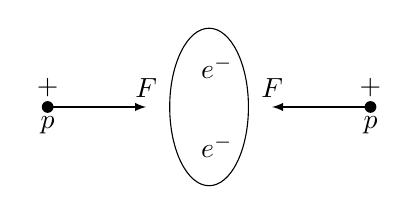
\begin{tikzpicture}
\draw (0,0) ellipse (0.5cm and 1cm);
\draw (0.1,0.5) node[]{$e^-$};
\draw (0.1,-0.5) node[]{$e^-$};
\draw[latex-] (-0.8,0) node[above]{$F$} --++ (-1.25,0) node[circle, fill, inner sep=1.5pt]{} node[below]{$p$} node[above]{$+$};
\draw[latex-] (0.8,0) node[above]{$F$} --++ (1.25,0) node[circle, fill, inner sep=1.5pt]{} node[below]{$p$} node[above]{$+$};
\end{tikzpicture}
\caption{}
\end{subfigure}\hfill
\begin{subfigure}{0.55\textwidth} 
\centering
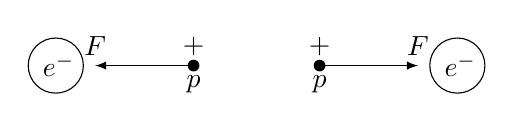
\begin{tikzpicture}
\draw[-latex] (-0.8,0) node[circle, fill, inner sep=1.5pt]{} node[below]{$p$} node[above]{$+$} --++ (-1.25,0) node[above]{$F$};
\draw[-latex] (0.8,0) node[circle, fill, inner sep=1.5pt]{} node[below]{$p$} node[above]{$+$} --++ (1.25,0) node[above]{$F$};
\draw (-0.8, 0) ++ (-1.25,0) ++ (-0.5,0) node[xshift=0.25ex]{$e^-$} circle (0.35);
\draw (0.8, 0) ++ (1.25,0) ++ (0.5,0) node[xshift=0.25ex]{$e^-$} circle (0.35);
\end{tikzpicture}
\caption{}
\end{subfigure}
\caption{شریک گرفتی بندھ کی نقشہ کشی: (ا)  تشاکلی تشکیل  قوت کشش پیدا کرتی ہے، (ب)  خلاف تشاکلی تشکیل  قوت دفع پیدا کرتی ہے۔}
\label{شکل_دو_اجزا_تشاکل_اور_خلاف_تشاکل_تشکیل}
\end{figure}


دلچسپ صورت تب پیدا ہوتی ہے جب انکے  تفاعلات موج   جزوی منطبق ہوں۔ ایسی صورت میں نظام کا رویہ کچھ یوں ہوگا جیسے متماثل بوزان کے بیچ  "قوت کشش"پائی جاتی ہو،  جو انہیں قریب کھینچتی ہے،  اور  متماثل فرمیان کے بیچ "قوت دفع" پائی  جاتی ہے،  جو انہیں ایک دوسرے سے دور دھکا  دیتے ہیں ( یاد رہے کہ ہم فی الحال چکر کو نظرانداز کر رہے ہیں)۔ ہم اس کو  \اصطلاح{قوت مبادلہ}\فرہنگ{قوت مبادلہ}\حاشیہب{exchange force}\فرہنگ{exchange force} کہتے ہیں اگرچہ یہ حقیقتاً ایک قوت نہیں ہے؛ کوئی بھی چیز ان ذرات کو دکھیل نہیں رہی ہے؛  یہ صرف ضرورت تشاکلیت کا \ترچھا{ہندسی}  نتیجہ ہے۔  ساتھ ہی یہ کوانٹم میکانی مظہر ہے جس کا کلاسیکی میکانیات میں کوئی مماثل نہیں پایا جاتا ہے۔ بہرحال اس کے دور رس  نتائج پائے جاتے ہیں۔ مثلاً،  ہائیڈروجن سالمہ \عددی{(\ce{H_2})} پر غور کریں۔ اندازاً بات کرتے ہوئے،  جوہری زمینی حال   (مساوات \حوالہ{مساوات_تین_ابعاد_زمینی_ہائیڈروجن})   جس کا مرکز مرکزہ \عددی{1} پر واقع ہے، میں ایک الیکٹران اور  جوہری زمین حال جس کا مرکز مرکزہ \عددی{2} پر واقع ہے،   میں ایک الیکٹران  پر زمینی حال مشتمل ہوگا۔ اگر الیکٹران بوزان ہوتے تب ضرورت تشاکلیت  (یا  "قوت مبادلہ" ، اگر آپ اسے پسند کرتے ہیں) کوشش کرتی ہے کہ دونوں پروٹان کے بیچ الیکٹرانوں کو جمع کرے
 (شکل \حوالہ{شکل_دو_اجزا_تشاکل_اور_خلاف_تشاکل_تشکیل}-ا)  ، نتیجتاً منفی بار کا انبار دونوں پروٹان کو اندر کی طرف ایک دوسرے کی جانب کھینچتا ہے،  جو \اصطلاح{شریک گرفتی بندھ}\فرہنگ{شریک گرفتی بند}\حاشیہب{covalent bond}\فرہنگ{covalent bond} کا سبب بنتا ۔\حاشیہد{مراکزہ کے بیچ  شراکتی الیکٹران جمع ہو کر جوہروں کو قریب کھینچ کر  شریک گرفتی بند پیدا  کرتے ہیں۔ اس کے لئے دو عدد الیکٹران لازمی نہیں ۔ ہم حصہ \حوالہ{حصہ_تغیری_اصول_ہائیڈروجن_بارداریہ} میں  صرف ایک الیکٹران پر مبنی شریک گرفتی بند دیکھیں گے۔  }  بدقسمتی سے  الیکٹران  در حقیقت  فرمیان ہیں نہ کہ بوزان جس کی بنا    پر منفی بار   اطراف پر انبار  ہو گا   (شکل \حوالہ{شکل_دو_اجزا_تشاکل_اور_خلاف_تشاکل_تشکیل}-ب)   جو سالمہ کو  ٹکڑے ٹکڑے کر دے  گا!

ذرا رکیے گا!   ہم چکر کو نظرانداز کرتے رہے ہیں۔ الیکٹران کا مقامی  تفاعل موج   اور      چکردار (جو الیکٹران کے چکر کی سمت بندی کو بیان کرتا ہے) مل کر اس کا  (درج ذیل)  مکمل حال دیں گے۔\حاشیہد{چکر اور مقام کے بیچ  عدم ارتباط کی صورت میں  ہم  فرض کر سکتے ہیں کہ چکر اور فضائی  محدد میں حال کو علیحدہ کرنا ممکن ہے۔اس سے مراد یہ ہے کہ ہم میدان چکر حاصل کرنے کا احتمال،  ذرے کے مقام پر منحصر نہیں ہو گا۔ ارتباط کی موجودگی میں عمومی حال، سوال \حوالہ{سوال_تین_ابعادی_چکر_و_مقام_مکین} کی طرز پر،  خطی ملاپ \عددی{\psi_+(\kvec{r})\chi_+ +\psi_{-}(\kvec{r})\chi_{-}} کا روپ اختیار کرے گا۔}
\begin{align}
	\psi(\kvec{r})\chi(\kvec{s})
\end{align}
دو الیکٹرانی حال مرتب کرتے  ہوئے ہمیں  مبادلہ کے لحاظ سے   صرف فضائی جزو کو عدم تشاکلی  نہیں   بلکہ  مکمل حال  کو   عدم تشاکلی بنانا ہوگا۔ مرکب چکری حالات (مساوات \حوالہ{مساوات_تین_ابعادی_سہ_تا_حال}  اور مساوات \حوالہ{مساوات_تین_ابعادی_یک_تا_حال})   پر نظریں ڈالتے ہوئے ہم دیکھتے ہیں کہ یک تا ملاپ خلاف تشاکل ہے ( لہٰذا اس کو تشاکل فضائی تفاعل کے ساتھ جوڑنا ہوگا)  جبکہ تینوں  سہ تا حالات تشاکلی ہیں (لہٰذا انہیں خلاف تشاکل فضائی تفاعل کے ساتھ منسلک کرنا ہوگا)۔ ظاہر ہے کہ یوں یکتا حال بندھ   پیدا کرے گا جبکہ سہ تا حال خلاف بندھ  ہوگا۔ یقیناً  کیمیا دان  ہمیں بتاتے ہیں کہ شریک گرفتی بندھ کے لئے ضروری ہے کہ دونوں الیکٹران یک تا حال کے مکین ہوں اور  ان کا کل چکر صفر ہو۔\حاشیہد{بے احتیاطی  میں ہم عموماً کہتے ہیں کہ الیکٹران ایک دوسرے کے مخالف صف بند ہیں (ایک ہم میدان اور دوسرا خلاف میدان)۔ یہ ضرورت سے زیادہ سادہ صورت ہو گی چونکہ یہی کچھ \عددی{m=0} سہ تا حال کے  بارے میں بھی کہا جا سکتا ہے۔درست  فقرہ یہ ہو گا:" وہ  یک تا تشکیل  میں ہیں"۔}


%below is prob 5.6 to prob 5.23 
%========================

%page 210
\ابتدا{سوال}
لامتناہی چکور کنواں میں دو  غیر متعامل ذرات جن میں سے ہر ایک کی کمیت  \عددی{m} ہے پائے جاتے ہیں۔ ان میں سے ایک حال \عددی{ \psi_{n}}  (مساوات \حوالہ{مساوات_شروڈنگر_میری_سائے})   اور دوسرا حال \عددی{  \psi _{l} }  \عددی{( l\neq n) }  میں ہے۔ \عددی{\langle  (x_{1} - x_{2})^2 \rangle} کا حساب اس صورت لگائیں  جب (الف)  ذرات  غیر قابل ممیز ہوں،  (ب) ذرات  متماثل بوزان ہوں اور (ج)  ذرات متماثل فرمیان ہوں۔
\انتہا{سوال}
\ابتدا{سوال}
فرض کریں آپ کے پاس تین ذرات ہیں جن میں سے ایک حال \عددی{ \psi_{a} }،  دوسرا حال \عددی{ \psi_{b} }،  اور تیسرا حال \عددی{ \psi_{c} } میں پایا  جاتا  ہے۔حالات \عددی{ \psi_{a} } ، \عددی{ \psi_{b} }،  اور \عددی{ \psi_{c} } کو معیاری عمودی تصور کرتے  ہوئے   (مساوات  \حوالہ{مساوات_متماثل_مجموعی_تفاعل_موج_قابل_ممیز}،  \حوالہ{مساوات_متماثل_مجموعی_تفاعل_موج_متماثل_بوزان} اور \حوالہ{مساوات_متماثل_مجموعی_تفاعل_موج_متماثل_فرمیان}  کی طرز پر)  تین  ذرہ حالات تیار کریں جو (الف) قابل ممیز ذرات ،  (ب) متماثل بوزان اور (ج) متماثل فرمیان کو ظاہر کرتے ہوں۔ یاد رہے کہ کسی بھی دو ذرات کی جوڑی کے باہمی مبادلہ کے لحاظ سے (ب) کو مکمل طور پر تشاکلی ہونا ہوگا،  جبکہ (ج)کو مکمل طور پر خلاف تشاکلی ہونا ہوگا۔ \ترچھا{تبصرہ:}  مکمل طور پر خلاف تشاکلی تفاعلات موج تیار کرنے کا ایک بہترین طریقہ پایا جاتا ہے۔\اصطلاح{  مقطع سلیٹر }\فرہنگ{مقطع!سلیٹر}\حاشیہب{Slater determinant}\فرہنگ{determinant!Slater}   تیار کریں جس کی پہلی صف  \عددی{ \psi_{a}(x_{1}) } ، \عددی{ \psi_{b}(x_{1}) } ، \عددی{ \psi_{c}(x_{1}) }،  وغیرہ  ہو گی،  اس کی دوسری صف \عددی{ \psi_{a}(x_{2}) } ، \عددی{ \psi_{b}(x_{2}) } , \عددی{ \psi_{c}(x_{2}) }، وغیرہ ہو گی اور اسی طرح اس کے باقی صف ہوں گے (یہ طریقہ  کسی بھی تعداد کے ذرات کیلۓ کارآمد ہے)۔
\انتہا{سوال}

\حصہ{جوہر}
ایک معادل جوہر جس کا جوہری عدد \عددی{Z} ہو، ایک بھاری مرکزہ جس کا بار  \عددی{Ze} ہو اور جس کو   ( کمیت  \عددی{m}  اور بار \عددی{ e-} کے)  \عددی{ Z} الیکٹران گھیرتے  ہوں پر مشتمل ہوگا۔ اس نظام کا ہیملٹنی درج ذیل ہو گا۔\حاشیہد{مرکزہ کو ساکن تصور کیا گیا ہے۔مرکزہ کی حرکت کو    تخفیف شدہ کمیت  (سوال  \حوالہ{سوال_متماثل_تخفیف_شدہ_کمیت}) کے ذریعہ  شامل کرنا صرف دو جسمی نظام کے لئے ممکن  ہے؛ خوش قسمتی سے مرکزہ کی کمیت الیکٹران کی کمیت سے اتنی زیادہ ہوتی ہے کہ  درکار درستگی، ہائیڈروجن کے لئے بھی، قابل نظر انداز ہوتی ہے (سوال \حوالہ{سوال_متماثل_درستگی}-ا دیکھیں)، اور زیادہ بھاری  جوہروں  کے لئے یہ  مزید کم ہو گی۔ مرکزہ کی  متناہی جسامت، اضافیتی درستگیاں اور الیکٹران چکر کے ساتھ وابستہ مقناطیسی باہم عمل کے زیادہ دلچسپ اثرات پائے جاتے ہیں۔ ان پر آنے والے ابواب میں غور کیا جائے گا، تاہم یہ تمام    "خالص کولمب" جوہر، جسے مساوات \حوالہ{مساوات_متماثل_ہیملٹنی_جوہر_عمومی} بیان کرتی ہے،  میں  انتہائی چھوٹی  درستگیاں    ہیں۔   }
%page 211
\begin{align}\label{مساوات_متماثل_ہیملٹنی_جوہر_عمومی}
H=\sum_{j=1}^{Z} \big\{ -\frac{h^2}{2m}\nabla_j^2-\big(\frac{1}{4\pi\epsilon_{0}}\big)  \frac{Ze^2}{r_{j}} \big\} + \frac{1}{2}\big(\frac{1}{4\pi\epsilon_{0}}\big) \sum_{j\ne  k}^{Z} \frac{e^2}{|\kvec{r}_{j} - \kvec{r}_{k} |}
\end{align}
 قوسین میں بند جزو،مرکزہ کے برقی میدان میں \عددی{ j} ویں  الیکٹران کی حرکی توانائی جمع مخفی توانائی کو ظاہر کرتا ہے؛  دوسرا  مجموعہ   (جو  ما سوائے \عددی{ j=k}،  تمام \عددی{ j} اور \عددی{ k} پر   لیا گیا ہے)   الیکٹرانوں کی  باہمی قوت دفع  سے وابستہ مخفی   توانائی کو ظاہر کرتا ہے ( جہاں \عددی{ \frac{1}{2}} اس حقیقت کو درست کرتا ہے کہ مجموعہ لیتے ہوئے ہر جوڑی کو دو بار گنا  گیا ہے)۔ ہمیں 
 تفاعل موج \عددی{ \psi(\kvec{r}_{1} , \kvec{r}_{2}, ...\kvec{r}_{Z}) } کیلۓ درج ذیل شروڈنگر مساوات:
\begin{align}\label{مساوات_متماثل_شروڈنگر_عمومی_جوہر}
 H\psi=E\psi
\end{align}
 حل کرنی ہوگی۔ البتہ  الیکٹران متماثل فرمیان ہیں، لہٰذا،  تمام حل قابل قبول نہیں ہوں گے: صرف وہ حل قابل قبول ہوں گے جن میں  مکمل حال  (مقام اور چکر):
\begin{align}
 \psi(\kvec{r}_{1},\kvec{r}_{2},...,\kvec{r}_{z}) \chi(\kvec{s}_{1},\kvec{s}_{2},\cdots,\kvec{s}_{Z}), 
\end{align}
کسی بھی دو الیکٹران کے باہمی مبادلہ کے لحاظ سے خلاف تشاکلی ہو۔ بالخصوص کوئی بھی دو الیکٹران ایک ہی حال کے مکین نہیں ہو سکتے ہیں۔

 بدقسمتی سے شروڈنگر مساوات کو مساوات \حوالہ{مساوات_متماثل_ہیملٹنی_جوہر_عمومی} میں دی گئی ہیملٹنی کے لئے،   ما سوائے سادہ ترین صورت \عددی{ Z=1}(  ہائیڈروجن)،    ٹھیک حل نہیں کیا جا سکتا ہے ( کم از کم آج تک کوئی بھی ایسا نہیں کر پایا ہے)۔ عملاً ہمیں  پیچیدہ تخمینی تراکیب استعمال کرنے ہوں گے۔ ان میں سے چند ایک تراکیب پر اگلے ابواب  میں غور کیا جائے گا؛  ابھی میں الیکٹران کی قوت دفع کو مکمل  نظر انداز کرتے ہوئے حلوں کا کیفی تجزیہ پیش کرنا چاہوں گا۔ حصہ  \حوالہ{حصہ_متماثل_ہیلیم}  میں ہم ہیلیم کے  زمینی حال اور ہیجان  حالات پر غور کریں گے  جبکہ حصہ \حوالہ{حصہ_متماثل_دوری_جدول}  میں ہم زیادہ بڑے  جوہر  کے زمینی حالات پر غور کریں گے۔

\ابتدا{سوال}
فرض کریں مساوات \حوالہ{مساوات_متماثل_ہیملٹنی_جوہر_عمومی}   میں دی گئی ہیملٹنی کے لیے آپ شروڈنگر مساوات (  مساوات  \حوالہ{مساوات_متماثل_شروڈنگر_عمومی_جوہر})    کا 
حل \عددی{( \psi(\kvec{r}_{1} , \kvec{r}_{2}, \kvec{r}_{3},...\kvec{r}_{Z}))} حاصل کر  سکتے ہیں۔ آپ اس سے ایک ایسا مکمل تشاکلی تفاعل اور  ایک مکمل خلاف تشاکلی تفاعل کس طرح بنا پائیں گے جو شروڈنگر مساوات کو اسی توانائی کیلۓ مطمئن کرتا ہو۔
\انتہا{سوال}
%page 212 
\جزوحصہ{ہیلیم}\شناخت{حصہ_متماثل_ہیلیم}
ہائیڈروجن کے بعد سب سے  سادہ جوہر ہیلیم \عددی{ (Z=2) } ہے۔ اس کا ہیملٹنی
\begin{align}\label{مساوات_متماثل_ہیلیم_ہیملٹنی}
H= \big\{ -\frac{h^2}{2m}\nabla^2 _{1} -\frac{1}{4\pi\epsilon_{0}} \frac{2e^2}{r_{1}}\big\} +
 \big\{ -\frac{h^2}{2m} \nabla^2 _{2}-\frac{1}{4 \pi \epsilon_{0}} \frac{2e^2}{r_{2}}\big\}+ \frac{1}{4 \pi \epsilon_{0}}\frac{e^2}{|\kvec{r}_{1} -\kvec{r}_{2}|}
\end{align}
(بار \عددی{ 2e}  مرکزہ کے)  دو   \ترچھا{ہائیڈروجنی}  ہیملٹنی، ایک  الیکٹران \عددی{1 }اور ایک  الیکٹران \عددی{2 }،  کے ساتھ دو الیکٹران کے بیچ توانائی دفع پر مشتمل ہو گا۔ یہ آخری جزو ہماری پریشانیوں کا سبب بنتا ہے۔ اس کو نظرانداز کرتے ہوئے مساوات  شروڈنگر قابل علیحدگی ہوگی   اور اس کے حلوں کو نصف بوہر رداس (مساوات \حوالہ{مساوات_تین_ابعادی_رداس_بوہر})   اور چار گنا بوہر توانائیوں (مساوات\حوالہ{مساوات_ابعادی_ہائیڈروجن_اجازتی_توانائیاں}) [  وجہ   سمجھ نہ آنے    کی صورت میں سوال \حوالہ{سوال_تین_ابعادی_ہائیڈروجنی_جوہر} پر دوبارہ نظر ڈالیں] کے  ہائیڈروجن تفاعلات موج کے حاصل ضرب :
\begin{align}
 \psi(\kvec{r}_{1}, \kvec{r}_{2})= \psi_{nlm} (\kvec{r}_{1}) \psi_{n' l' m'} (\kvec{r}_{2})
\end{align}
کی صورت میں لکھا جا سکتا ہے۔ کل توانائی درج ذیل ہوگی جہاں \عددی{ E_{n}=-13.6/n^2 \,\si{\electronvolt} } ہوگا۔
\begin{align}
 E= 4(E_{n} +E_{n'})
 \end{align}
بالخصوص زمینی حال 
\begin{align}\label{مساوات_متماثل_ہیلیم_زمینی_حال}
\psi_{0}(\kvec{r}_{1}, \kvec{r}_{2})=\psi_{100}(\kvec{r}_{1}) \psi_{100}(\kvec{r}_{2})=\frac{8}{\pi a^3}e^{-2(r_{1} + r_{2})/a}
\end{align}
ہو گا (مساوات  \حوالہ{مساوات_تین_ابعاد_زمینی_ہائیڈروجن}  دیکھیں) اور اس کی توانائی درج ذیل ہوگی۔
\begin{align}\label{مساوات_متماثل_ہیلیم_توانائی_الف}
 E_{0}=8(\SI{-13.6}{\electronvolt})=\SI{-109}{\electronvolt}
 \end{align}
چونکہ \عددی{ \psi_{0} } تشاکلی تفاعل ہے لہٰذا چکری  حال کو \ترچھا{خلاف تشاکلی} ہونا ہوگا اور یوں ہیلیم کا  زمینی حال   \ترچھا{یک تا} تشکیل میں   ہوگا،  جس میں چکر ایک دوسرے کے "مخالف صف بند" ہوں گے۔ یقیناً حقیقت میں ہیلیم کا زمینی حال   یک تا  ہی ہے،  تاہم  اس کی تجرباتی  حاصل  توانائی  \عددی{\SI{-78.975}{\electronvolt}} ہے  جو مساوات \حوالہ{مساوات_متماثل_ہیلیم_توانائی_الف} سے کافی مختلف ہے۔ یہ زیادہ  حیرت کی بات نہیں ہے:  ہم نے الیکٹران کی توانائی دفع کو مکمل طور پر نظرانداز کیا جو چھوٹی مقدار نہیں ہے۔ یہ ایک مثبت مقدار   (مساوات \حوالہ{مساوات_متماثل_ہیلیم_ہیملٹنی}  دیکھیں) ہے  جس کو شامل کرتے ہوئے کل توانائی کم  ہو کر     \عددی{\SI{-109}{\electronvolt}}  کی بجائے  \عددی{\SI{-79}{\electronvolt}}  ہو جائے گی  (سوال \حوالہ{سوال_متماثل_توانائی_دفع}  دیکھیں)۔

 ہیلیم  کے ہیجان حالات: 
\begin{align}
 \psi_{nlm} \psi_{100}
 \end{align}
ہائیڈروجنی زمینی حال میں ایک الیکٹران اور    ہیجان حال میں دوسرے  الیکٹران، پر  مشتمل ہوگا۔[ دونوں الیکٹران کو ہیجان حالات میں ڈالنے سے  ایک الیکٹران   فوراً  زمینی حال میں واپس گر کر توانائی خارج کرتا ہے، جو دوسرے الیکٹران کو جوہر سے باہر استمراریہ \عددی{ (E>0)} میں  دھکیلتا ہے  ، اور  یوں ایک آزاد الیکٹران اور ہیلیم بارداریہ \عددی{ (\ce{He^+} ) } حاصل ہوگا۔ یہ بذات خود ایک دلچسپ نظام ہے جس پر ہم یہاں بات نہیں کر رہے ہیں؛ سوال \حوالہ{سوال_متماثل_دھکیلنا}  دیکھیں]  ہم ہمیشہ کی طرح تشاکلی اور خلاف تشاکلی   ملاپ  تیار کر سکتے ہیں ( مساوات \حوالہ{مساوات_متماثل_غیر_مشروط_حال});  اول الذکر خلاف تشاکلی چکر تشکیل  (یک تا) کے ساتھ جائے گا،  جنہیں \اصطلاح{ نزدہیلیم}\فرہنگ{نزدہیلیم}\حاشیہب{parahelium}\فرہنگ{parahelium} کہتے ہیں،  جبکہ موخر الذکر کو تشاکلی چکر  تشکیل ( سہ تا)  درکار ہوگی اور انہیں  \اصطلاح{ ہیلیم  پرست}\فرہنگ{ہیلیم پرست}\حاشیہب{orthohelium}\فرہنگ{orthohelium}  کہتے ہیں۔ زمینی حال لازماً نزدہیلیم ہوگا؛ جبکہ ہیجان حالات دونوں روپ میں پائے جاتے ہیں۔ جیسا ہم نے حصہ  \حوالہ{حصہ_متماثل_قوت_مبادلہ}  میں دریافت کیا، تشاکلی فضائی حال الیکٹرانوں  کو قریب لاتا  ہے،  جس کی بنا پر  ہم توقع کرتے ہیں کہ نزدہیلیم کی باہم متعامل توانائی زیادہ ہوگی، اور  یقیناً تجربات سے تصدیق ہوتی ہے کہ ہیلیم پرست کے لحاظ سے نزدہیلیم حالات کی توانائی زیادہ ہے ( شکل \حوالہ{شکل_متماثل_ہیلیم_توانائیاں}  دیکھیں)۔

\begin{figure}
\centering
\begin{tikzpicture}
\pgfmathsetmacro{\kx}{1}
\pgfmathsetmacro{\ky}{1.25}
\draw[](0,0)node[left]{$0$}--++(9.5*\kx,0);
\draw[thick](0,0)--++(0,-5.5*\ky)node[pos=0.5,xshift=-1cm,rotate=90,]{\RL{توانائی $(\si{\electronvolt})$}};
\foreach \k in {-1,-2,-3,-4,-5}{\draw(0,\ky*\k)node[left]{$\k$}--++(0.1,0);}
\draw[-stealth](\kx,0)node[above]{$^1S$}--++(0,-5.25*\ky)node[below right,xshift=-1.5em]{\RL{(\عددی{\SI{-24.5}{\electronvolt}} پر \عددی{1S})}};
\foreach \k/\t in {-0.914/4S,-1.68/3S,-3.96/2S}{\draw(1*\kx-0.1,\ky*\k)node[left]{$\t$}--++(0.2,0);}
\draw[](2*\kx,0)node[above]{$^1P$}--++(0,-3.36*\ky);
\foreach \k/\t in {-0.93/4P,-1.71/3P,-3.36/2P}{\draw(2*\kx-0.1,\ky*\k)node[left]{$\t$}--++(0.2,0);}
\draw[](3*\kx,0)node[above]{$^1D$}--++(0,-1.5*\ky);
\foreach \k/\t in {-0.86/4D,-1.5/3D}{\draw(3*\kx-0.1,\ky*\k)node[left]{$\t$}--++(0.2,0);}
\draw[](4*\kx,0)node[above]{$^1F$}--++(0,-0.85*\ky);
\foreach \k/\t in {-0.85/4F}{\draw(4*\kx-0.1,\ky*\k)node[left]{$\t$}--++(0.2,0);}
\draw[](6*\kx,0)node[above]{$^3S$}--++(0,-4.79*\ky);
\foreach \k/\t in {-0.96/4S,-1.86/3S,-4.79/2S}{\draw(6*\kx-0.1,\ky*\k)node[left]{$\t$}--++(0.2,0);}
\draw[](7*\kx,0)node[above]{$^3P$}--++(0,-3.64*\ky);
\foreach \k/\t in {-0.86/4P,-1.56/3P,-3.64/2P}{\draw(7*\kx-0.1,\ky*\k)node[left]{$\t$}--++(0.2,0);}
\draw[](8*\kx,0)node[above]{$^3D$}--++(0,-1.5*\ky);
\foreach \k/\t in {-0.86/4D,-1.5/3D}{\draw(8*\kx-0.1,\ky*\k)node[left]{$\t$}--++(0.2,0);}
\draw[](9*\kx,0)node[above]{$^3F$}--++(0,-1.2*\ky);
\foreach \k/\t in {-1.2/4F}{\draw(9*\kx-0.1,\ky*\k)node[left]{$\t$}--++(0.2,0);}
\draw[decorate,decoration={brace,amplitude=5pt,raise=15pt}](0,0)--++(4.25*\kx,0)node[pos=0.5,yshift=1cm]{نزدہیلیم};
\draw[decorate,decoration={brace,amplitude=5pt,raise=15pt}](5.75*\kx,0)--++(4*\kx,0)node[pos=0.5,yshift=1cm]{\RL{ہیلیم پرست}};
\end{tikzpicture}
\caption{
ہیلیم کی توانائیوں کے سطح (علامتیت کی وضاحت حصہ \حوالہ{حصہ_متماثل_دوری_جدول} کی گئی ہے)۔ آپ دیکھ سکتے ہیں کہ نزدہیلیم کی توانائیاں مطابقتی  ہیلیم پرست سے  زیادہ ہیں۔انتصابی پیمانہ  باردارہ ہیلیم  کے زمینی حال 
\عددی{(\ce{He^+}:4\times (-13.6)\si{\electronvolt}=\SI{-54.4}{\electronvolt})}  کے لحاظ سے ہیں۔؛ کسی بھی حال کی کل توانائی جاننے کی خاطر \عددی{\SI{54.4}{\electronvolt}} منفی کریں۔
}
\label{شکل_متماثل_ہیلیم_توانائیاں}
\end{figure}

%page 214 
\ابتدا{سوال}\شناخت{سوال_متماثل_دھکیلنا}
\begin{enumerate}[a.]
\item
فرض کریں کہ آپ ہیلیم  جوہر کے دونوں الیکٹران کو \عددی{ n=2} حال میں رکھتے ہیں؛ خارجی  الیکٹران کی توانائی کیا ہوگی؟
\item
ہیلیم بارداریہ \عددی{ \ce{He^+}} کے طیف پر  (مقداری)  تجزیہ کریں۔ 
\end{enumerate}
\انتہا{سوال}
\ابتدا{سوال}
ہیلیم کی توانائیوں کی سطح پر درج ذیل صورت میں (کیفی) تجزیہ کریں۔ (ا) اگر الیکٹران متماثل بوزان ہوتے،  (ب) اگر الیکٹران قابل ممیز ذرات  ہوتے ( لیکن   ان کی کمیت اور بار  ایک جیسے ہوں)۔ فرض کریں کہ الیکٹران کا چکر اب بھی \عددی{ \frac{1}{2} }  ہے  لہٰذا   چکری  تشکیلات یک تا اور سہ تا ہوں  گے۔
\انتہا{سوال}
\ابتدا{سوال}\شناخت{سوال_متماثل_توانائی_دفع}
\begin{enumerate}[a.]
\item
مساوات   \حوالہ{مساوات_متماثل_ہیلیم_زمینی_حال}  میں دیے گئے  حال \عددی{ \psi_{0} }  کیلۓ  \عددی{ \langle(1/|\kvec{r}_{1} - \kvec{r}_{2}|)\rangle} کا حساب لگائیں۔ \ترچھا{ اشارہ:}  کروی محدد استعمال کرتے ہوئے قطبی محور کو \عددی{ \kvec{r}_{1} } پر رکھیں  تا کہ
\begin{align}
|\kvec{r}_{1}-\kvec{r}_{2}|= \sqrt{r_1^2+ r_2^2 -2r_{1} r_{2}\cos\theta_{2}}.
\end{align}
ہو۔ پہلے  \عددی{ \dif^{\,^3} \kvec{r}_{2}}   کا تکمل حل کریں۔ زاویہ    \عددی{ \theta_{2} }    کے لحاظ سے تکمل آسان ہے، بس مثبت جذر لینا  یاد رکھیں۔ آپ کو      \عددی{ r_{2} }     تکمل دو ٹکڑوں میں تقسیم کرنا ہوگا؛ پہلا \عددی{0}سے      \عددی{ r_{1} }      تک اور دوسرا       \عددی{ r_{1} } سے \عددی{ \infty } تک۔ جواب: \عددی{\frac{5}{4a} } 
\item
جزو -ا  کا نتیجہ استعمال کرتے ہوئے ہیلیم کے زمینی حال میں الیکٹران کی باہمی متعامل توانائی کا اندازہ لگائیں۔ اپنے جواب کو الیکٹران وولٹ کی صورت میں پیش کریں اور اس کو \عددی{ E_{0}} (مساوات  \حوالہ{مساوات_متماثل_ہیلیم_توانائی_الف})  کے ساتھ جمع کر کے زمینی حال توانائی کی بہتر تخمین  حاصل کریں۔ اس کا موازنہ تجرباتی قیمت کے ساتھ کریں۔ (دھیان رہے کہ اب بھی آپ تخمینی تفاعل موج کے ساتھ کام کر رہے ہیں،  لہٰذا آپ کا جواب ٹھیک تجرباتی جواب نہیں ہوگا۔  )
\end{enumerate}
\انتہا{سوال}

%KKK edited till here 17 dec 2021
\جزوحصہ{دوری جدول}\شناخت{حصہ_متماثل_دوری_جدول}
بھاری جوہروں کے زمینی حال الیکٹرانی تشکیل اسی طرح جوڑ کر حاصل کیے جاتے ہیں۔ پہلی تخمین  میں( انکی باہمی توانائی دفع کو مکمل نظرانداز کرتے ہوئے)  بار \عددی{Z_e} کے مرکزہ کے کولمب مخفیہ میں یک  ذروی ہائیڈروجنی حالات \عددی{(n, l, m)}،  جنہیں مدارچے کہتے ہیں، کے  انفرادی الیکٹران مکین ہوں گے۔ اگر الیکٹران بوزان (یا قابل  ممیز ذرات ) ہوتے تب یہ زمینی حال \عددی{(1, 0, 0)} میں  گر جاتے اور کیمیا اتنا دلچسپ نہ ہوتا۔ حقیقت میں الیکٹران متماثل فرمیان ہیں، جن پر پالی اصول مناعت لاگو ہوتا ہے،  لہٰذا کسی ایک مدارچہ کے  صرف دو الیکٹران مکین ہو   سکتے ہیں  (ایک ہم میدان اور ایک خلاف میدان ؛ بلکہ یہ کہنا زیادہ بہتر  ہو گا ، کہ   یک تا  تشکیل  میں  )۔ کسی بھی \عددی{n} کی قیمت کے لئے \عددی{n^2} ہائیڈروجنی تفاعلات موج پائے جاتے ہیں  (جن میں سے ہر ایک کی توانائی \عددی{E_n} ہوگی)، یوں \عددی{n=1} \اصطلاح{خول}\فرہنگ{خول}\حاشیہب{shell}\فرہنگ{shell}  میں دو الیکٹرانوں کی جگہ ہو گی،  \عددی{n=2} خول میں آٹھ،  \عددی{n=3} میں اٹھارہ،  اور \عددی{n}ویں خول میں \عددی{2n^2} الیکٹرانوں کی جگہ ہوگی۔ کیفی طور پر بات کرتے ہوئے \اصطلاح{ دوری جدول}\فرہنگ{دوری جدول}\حاشیہب{periodic table}\فرہنگ{periodic table}  کے افقی صف،  انفرادی خول کو  بھرنے کے مترادف ہے ( اگرچہ یہ پوری کہانی نہیں ہے،  چونکہ ایسا ہونے کی صورت میں انکی لمبائیاں \عددی{2}،  \عددی{8}،  \عددی{18}،  \عددی{32}،  \عددی{50}،وغیرہ ہوتیں  نا کہ  \عددی{2}،  \عددی{8}،  \عددی{8}،  \عددی{18}،  \عددی{18}، وغیرہ ؛ ہم جلد دیکھیں گے کہ الیکٹران کا باہم   دفع اس شمار کو کس طرح خراب کرتا ہے)۔

ہیلیم میں ، \عددی{n=1} خول  بھرا ہوگا،  لہٰذا اگلا جوہر لتھیم \عددی{(Z=3)} کو ایک الیکٹران \عددی{n=2} خول میں رکھنا ہوگا۔ اب \عددی{n=2} کی صورت میں \عددی{l=0} یا \عددی{l=1} ہو سکتا ہے۔ تیسرا الیکٹران ان میں سے کس ایک کا انتخاب کرے گا؟ چونکہ بوہر توانائی \عددی{n} پر منحصر ہوتی ہے نا کہ \عددی{l} پر لہٰذا الیکٹران کا باہمی عمل نہ ہونے کی صورت میں ان دونوں کی توانائی ایک دوسرے جیسی ہوگی۔ تاہم درج ذیل وجہ کی بنا الیکٹران کی توانائی دفع  \عددی{l}  کی کم سے کم قیمت کی طرف داری کرتی ہے۔  زاویائی معیار حرکت الیکٹران کو بیرونی رخ دھکیلنے کی کوشش کرتا ہے اور الیکٹران جتنا  زیادہ  مرکزہ سے دور ہوگا  اتنا مرکزہ،  اندرونی الیکٹرانوں  کے زیادہ پس پردہ ہو  کر اوجھل ہو گا۔  ہم کہہ سکتے ہیں کہ اندرونی الیکٹران کو مرکزہ کا پورا  \عددی{Ze} نظر آتا ہے جب کہ بیرونی الیکٹران کو مشکل سے  \عددی{e}  سے زیادہ موثر  نظر آتا ہے ۔یوں کسی بھی ایک خول میں کم سے کم توانائی کا حال یعنی دوسرے لفظوں میں سب سے سخت مقید الیکٹران  \عددی{ l=0}   ہوگا ۔ اور بڑھتے   \عددی{l}   کے ساتھ توانائی بڑھے گی اس طرح لتھیم میں تیسرا الیکٹران مدارچہ   \عددی{(2,0,0)}  کا مقید ہوگا۔ اگلا جوہر بیریلیم جس کا   \عددی{Z=4}   ہے اسی حال میں ہوگا لیکن اس کا چکر مخالف رخ ہوگا لیکن بوران   \عددی{Z=5}   کو  \عددی{ l=1}   استعمال کرنا ہوگا۔ 
 %==================
 
 
 اسی طرح چلتے ہوئے ہم  نیون  \عددی{ Z=10}   تک پہنچتے ہیں جہاں   \عددی{n=2}   خول مکمل بھرا ہوگا اور ہم دوری جدول کی اگلی صف کو پہنچ کر   \عددی{n= 3}   خول کو بھرنا شروع کرتے ہیں ۔ آغاز میں دو جوہر سوڈیم اور مگنیشیم  ہیں جن کا  \عددی{ l=0}   ہے اور اس کے بعد سلور  سے آرگن تک چھ ایسے جوہر ہیں جن کے لیے   \عددی{L=1}   ہوگا۔ آرگن کے بعد ہم توقع کرتے ہیں کہ دس ایسے جوہر پائے جائیں گے جن کے لیے    \عددی{n=3}    اور    \عددی{l=2}    ہوگا البتہ یہاں پہنچ کر   اندرونی الیکٹران کا مرکزہ کو پس پردہ کرنے کا اثر اتنا زور پکڑتا ہے کہ اگلا خول بھی اس کے نظر ہو جاتا ہے (یعنی یہ خول بھی  اوجھل ہو  جاتا ہے)   لہٰذا  پوٹاشیم  \عددی{( Z=19)}    اور کلشیم   \عددی{(Z=20)}   ،   \عددی{(n=3),(l=2)}  کی بجائے  \عددی{ (n=4),( L=0 )}  منتخب کرتے ہیں  ۔ اس کے بعد ہم نیچے اتر کر اسکینڈیم سے  جست  تک کے جوہر اٹھاتے ہیں جن کے لیے  \عددی{ n=3}   اور \عددی{ l=2}    ہوگا ۔ اس کے بعد گیلیم سے کرپٹان تک \عددی{ n=4، l=1}     ہوگا جس کے آخر میں ہم دوبارہ قبل از وقت اگلی صف \عددی{ n=5}      کو چھلانگ لگاتے ہیں اور بعد میں واپس اتر کر \عددی{ n= 4}       خول کے ۔ وہ مدارجے جن کے لیے \عددی{ l=2، l=3}      ہوں پر کرتے ہیں ۔ یہاں جوہری حالات کے  تسمیہ  جس کو  تمام  کیمیا دان  اور ماہر طبیعیات  استعمال کرتے ہیں پر تبصرہ کرنا ضروری ہوگا اس کی وجہ شاید صرف انیسویں صدی کے تیز پیمائی کاروں کو معلوم ہوگا کہ  \عددی{l=0}      کو   \عددی{s}       کہتے ہیں   \عددی{l=1}        کو   \عددی{p}         کہتے ہیں، \عددی{ l=2}          کو    \عددی{d}           کہتے ہیں اور    \عددی{l=3}             کو \عددی{ f}   کہتے ہیں۔ میرے خیال سے اس کے بعد وہ سیدھی راس پر آ گئے اور انہوں نے حروف تہجی کے تحت \عددی{ (g,h,i,,k,l)}    وغیرہ نام دینا شروع کیا۔ انہوں نے ہماری ناک میں دم کرنے کی خاطر    \عددی{j}     کو نظر انداز کیا ۔ کسی ایک الیکٹران کے حال کو     \عددی{ (n,l)}      کی جوڑی ظاہر کرتی ہے جہاں عدد n حال کو اور حرف     \عددی{l}       مدارجی زاویائی معیار حرکت کو ظاہر کرتا ہے ۔ کوانٹم عدد    \عددی{m}        کا  ذکر نہیں کیا جاتا لیکن قوت نما میں حال کے مکین الیکٹرانوں کی تعداد لکھی جاتی ہے ۔ یوں درج ذیل تشکیل
\begin{align}
(1s)^{2}(2s)^{2}(2p)^{2} 
\end{align}
کہتی ہے کہ مدارچہ \عددی{(1,0,0)}  میں 2 الیکٹران،  مدارچہ \عددی{( 2,0,0)}  میں 2 جبکہ مدارجے \عددی{( 2,1,1)} ،  \عددی{(2,1,0)}  اور  \عددی{(2,1,-1)}  کے کسی ملاپ میں 2 الیکٹران پائے جاتے ہیں ۔ یہ درحقیقت کاربن کا زمینی حل ہے ۔ 

 اس مثال میں 2 الیکٹران ایسے پائے جاتے ہیں جن کے مدارجی زاویائی معیار حرکت کوانٹم  عدد ایک ہے لہٰذا مدارچی زاویائی معیار حرکت کوانٹم عدد ایک ہے لہٰذا کل مدارچی زاویائی معیار حرکت کوانٹم نمبر  \عددی{l} کسی ایک ذروی کی جب  \عددی{L} کل قیمت کو ظاہر کرتا ہے ۔ ایک، دو یا صفر ہو  سکتا ہے۔ جبکہ  \عددی{(1s)}  کے دو   الیکٹران ایک دوسرے کے ساتھ یک تا حال  بندھن میں  ہیں اور ان کا کل چکر صفر ہوگا۔ یہی کچھ \عددی{( 2S)}  کے دو الیکٹران کے لئے بھی ہوگا لیکن  \عددی{(2p)}  کے دو الیکٹران یا تو یکتا نظام اور یا سہ تا نظام میں ہوں گے۔ یوں کل چکر کوانٹم عدد S کل کو ظاہر کرنے کے لئے بڑا حرف استعمال ہوگا۔ جس کی قیمت ایک یا صفر ہو سکتی ہے۔ ظاہر ہے میزان کل مدارچی جمع چکر J کی قیمت تین، دو، ایک یا صفر ہو سکتی ہے۔ کسی ایک جوہر کے لئے ان کل قیمتوں کو  قواعد  ہن ( سوال 5.1 دیکھیں)  سے حاصل کیا جا سکتا ہے ۔نتیجہ کو درجہ ذیل روپ میں لکھا جا سکتا ہے. 
 \begin{align}
 ^{2S+1}L_{J}\end{align}
  جہاں J اور S اعداد جبکہ L ایک حرف ہو گا اور چونکہ ہم کل کی بات کر رہے ہیں لہٰذا یہ بڑا حرف ہو گا کاربن کا زمینی حال  3D ہے جس کا کل چکر ایک ہے جس کی بنا 3 لکھا گیا ہے کل مدارچی زاویائی معیار حرکت ایک ہے لہٰذا
  \عددی{1p}    لکھا گیا ہے اور میزان  کل زاویائی معیار حرکت صفر ہے لہٰذا صفر لکھا گیا ہے۔ جدول  \حوالہ{جدول_متماثل_دوری_جدول_الیکٹران_تشکیل}  میں دوری جدول کے ابتدائی چار  صف  کے لئے انفرادی  تشکیلات  اور کل زاویائی معیار حرکت مساوات 5.34 کی روپ میں پیش کئے گئے ہیں ۔ 
  %Table 5.1 Page 229.
\begin{table}
\caption{دوری جدول  کے اولین چار  قطاروں کے  الیکٹران تشکیلات}
\label{جدول_متماثل_دوری_جدول_الیکٹران_تشکیل}
\centering
%\renewcommand{\arraystretch}{1.5}
\begin{tabular}{rlll}
\toprule
Z & عنصر &\multicolumn{2}{l}{
تشکیل
\quad\quad\quad}\\
\midrule
1 & \ce{H} & $(1s)$ & $^2S_{1/2}$\\
2 & \ce{He} & $(1s)^2$ & $^1S_{0}$\\
\midrule
3 & \ce{Li} & $(\ce{He})(2s)$ & $^2S_{1/2}$\\
4 & \ce{Be} & $(\ce{He})(2s)^2$ & $^1S_{0}$\\
\midrule
5 & \ce{B} & $(\ce{He})(2s)^2(2p)$ & $^2P_{1/2}$\\
6 & \ce{C} & $(\ce{He})(2s)^2(2p)^2$ & $^3P_{0}$\\
7 & \ce{N} & $(\ce{He})(2s)^2(2p)^3$ & $^4S_{3/2}$\\
8 & \ce{O} & $(\ce{He})(2s)^2(2p)^4$ & $^3P_{2}$\\
9 & \ce{F} & $(\ce{He})(2s)^2(2p)^5$ & $^2P_{3/2}$\\
10 & \ce{Ne} & $(\ce{He})(2s)^2(2p)^6$ & $^1S_{0}$\\
\midrule
11 & \ce{Na} & $(\ce{Ne})(3s)$ & $^2S_{1/2}$\\
12 & \ce{Mg} & $(\ce{Ne})(3s)^2$ & $^1S_{0}$\\
\midrule
13 & \ce{Al} & $(\ce{Ne})(3s)^2(3p)$ & $^2P_{1/2}$\\
14 & \ce{Si} & $(\ce{Ne})(3s)^2(3p)^2$    &    $^3P_{0}$\\
15 & \ce{P} & $(\ce{Ne})(3s)^2(3p)^3$    &    $^4S_{3/2}$\\
16 & \ce{S} & $(\ce{Ne})(3s)^2(3p)^4$    &    $^3P_{2}$\\
17 & \ce{Cl} & $(\ce{Ne})(3s)^2(3p)^5$    &    $^2P_{3/2}$\\
18 & \ce{Ar} & $(\ce{Ne})(3s)^2(3p)^6$    &    $^1S_{0}$\\
\midrule
19 & \ce{K} & $(\ce{Ar})(4s)$    &    $^2S_{1/2}$\\
20 & \ce{Ca} & $(\ce{Ar})(4s)^2$    &    $^1S_{0}$\\
\midrule
21 & \ce{Sc} & $(\ce{Ar})(4s)^2(3d)$    &    $^2D_{3/2}$\\
22 & \ce{Ti} & $(\ce{Ar})(4s)^2(3d)^2$    &    $^3F_{2}$\\
23 & \ce{V} & $(\ce{Ar})(4s)^2(3d)^3$    &    $^4F_{3/2}$\\
24 & \ce{Cr} & $(\ce{Ar})(4s)(3d)^5$    &    $^7S_{3}$\\
25 & \ce{Mn} & $(\ce{Ar})(4s)^2(3d)^5$    &    $^6S_{5/2}$\\
26 & \ce{Fe} & $(\ce{Ar})(4s)^2(3d)^6$    &    $^5D_{4}$\\
27 & \ce{Co} & $(\ce{Ar})(4s)^2(3d)^7$    &    $^4F_{9/2}$\\
28 & \ce{Ni} & $(\ce{Ar})(4s)^2(3d)^8$    &    $^3F_{4}$\\
29 & \ce{Cu} & $(\ce{Ar})(4s)(3d)^{10}$    &    $^2S_{1/2}$\\
30 & \ce{Zn} & $(\ce{Ar})(4s)^2(3d)^{10}$    &    $^1S_{0}$\\
\midrule
31 & \ce{Ga} & $(\ce{Ar})(4s)^2(3d)^{10}(4p)$    &    $^2P_{1/2}$\\
32 & \ce{Ge} & $(\ce{Ar})(4s)^2(3d)^{10}(4p)^2$    &    $^3P_{0}$\\
33 & \ce{As} & $(\ce{Ar})(4s)^2(3d)^{10}(4p)^3$    &    $^4S_{3/2}$\\
34 & \ce{Se} & $(\ce{Ar})(4s)^2(3d)^{10}(4p)^4$    &    $^3P_{2}$\\
35 & \ce{Br} & $(\ce{Ar})(4s)^2(3d)^{10}(4p)^5$    &    $^2P_{3/2}$\\
36 & \ce{Kr} & $(\ce{Ar})(4s)^2(3d)^{10}(4p)^6$    &    $^1S_{0}$\\
\bottomrule
\end{tabular}
\end{table}



\ابتدا{سوال}
  جزو  الف: دوری جدول کے ابتدائی  دو صف  کے لئے نیون  تک مساوات 5.33 کی روپ میں  الیکٹران تشکیلات  پیش کر کے ان کی تصدیق جدول  \حوالہ{جدول_متماثل_دوری_جدول_الیکٹران_تشکیل} کے ساتھ کریں ۔ \\
  جز ب :ابتدائی  چار عناصر  کے لئے مساوات  5.34 کی روپ میں ان کا مطابقتی کل زاویائی معیار حرکت تلاش کریں ۔بوران، کاربن اور نائیٹروجن کے لئے تمام ممکنات پیش کریں۔\\
\انتہا{سوال}
\ابتدا{سوال}
   جزو  الف: ہن کا پہلا قاعدہ کہتا ہے کہ باقی چیزیں ایک جیسا ہونے کے لیے صورت میں وہ حال جس کا کل چکری زیادہ سے زیادہ ہوگی کم سے کم توانائی ہو گی۔ ہیلیم کے ہیجان حالات کے لیے یہ کیا  پیشنگوئی کرتا ہے۔\\
    جزو  ب: ہن کا دوسرا قاعدہ کہتا ہے کہ کسی ایک چکر کی صورت میں مجموعی طور پر خلاف تشاکلیت پر پورا اترتا ہو۔ وہ حال جس کی مدارچی زاویائی معیار حرکت Ll زیادہ سے زیادہ ہو گی توانائی کم سے کم ہو گی ۔ کاربن کے لئے 2=L کیوں نہیں ہوگا؟ اشارہ سیڑھی کا بالائی سر
    \عددی{(M_{L}=L)}
      تشاکلی ہے۔\\
      جزو ج: ہن کا تیسرا قاعدہ کہتا ہے کہ اگر ایک ذیلی خول     \عددی{(n,l)}        نصف سے زیادہ بھرا نا ہو تب کم سے کم توانائی کی سطح کے لئے      \عددی{J=\abs{L-S}}         ہو گا۔ اگر یہ نصف سے زیادہ بھرا ہو تب \عددی{ J=L+S}  کی توانائی کم سے کم ہوگی۔ اس حقیقت کو استعمال کرتے ہوئے سوال 5.12 ب میں بوران کے مسئلہ سے شک دور کرے۔\\
        جزو  د: قواعد ہن کے ساتھ یہ حقیقت استعمال کرتے ہوئے کہ تشاکلی چکری حال کے ساتھ حال  خلاف تشاکلی مقام  کے ساتھ خلاف تشاکل چکر حال استعمال ہوگا ۔سوال 5.12 ب میں کاربن اور نائیٹروجن  میں درپیش مشکلات سے چھٹکارا حاصل کریں ۔ اشارہ کسی بھی حال کی تشاکلی جاننے کی خاطر سیڑھی کے بالائی سر سے آغاز کریں ۔
\انتہا{سوال}
 \ابتدا{سوال}
  دوری جدول کے چھٹے صف میں عنصر  \عددی{66} ڈسپروزیم کا زمینی حال   \عددی{^{5}I_{8}}    ہے۔ اس کے کل چکر کل مدارچے اور میزان کل زاویائی معیار حرکت کوانٹم کل حالات کیا ہوں گے۔ڈسپروزیم کے الیکٹران  تشکیل  کا خاکہ کیا ہو سکتا ہے۔
  \انتہا{سوال}
  
\حصہ{ٹھوس اجسام} 
ٹھوس حال میں ہر جوہر کے بیرونی ڈھیلے  مقید گرفتی الیکٹرانوں میں سے چند ایک علیحدہ ہو کر کسی مخصوص  "موروثی"  مرکزہ کے کولمب  میدان سے آزاد، تمام قلمی جال کے مخفیہ کے زیرِ اثر حرکت کرنا شروع کرتے ہے اس حصہ میں ہم   انتہائی  سادہ  نمونوں پر  غور کریں گے۔ پہلا نمونہ الیکٹران گیس نظریہ ہے جو سمرفلڈ نے پیش کیا اس نمونے میں سرحد کے اثرات کے علاوہ باقی تمام قوتوں کو نظرانداز کیا جاتا ہے اور الیکٹرانوں کو لامتناہی چکور کنواں کے تین آبادی مماثل کی طرح ڈبے میں آزاد ذرات تصویر کیا جاتا ہے۔ دوسرا نمونہ نظریہ  بلوخ   کہلاتا ہے الیکٹران کی باہمی دفع کو نظر انداز کرتے ہوئے باقاعدگی سے ایک جتنے فاصلے پر مثبت بار کے مرکزہ کو دوری مخفیہ سے ظاہر کرتا ہے، یہ نمونے ٹھوس اجسام کی کوانٹم نظریے کی طرف پہلے لڑکھڑاتے قدم ہیں۔ اس کے باوجود یہ پالی حصول مناعت کا جمود  میں گہرا کردار اور موصل، غیر موصل اور نیم موصل کی حیرت کن برقی خواص پر روشنی ڈالنے میں مدد دیتی ہے۔

\جزوحصہ{آزاد الیکٹران گیس}
،فرض کرے ایک ٹھوس جسم مستطیل شکل کا ہے جس کے اضلاع   \عددی{l_{x}}  ،  \عددی{l_{y}}   اور  \عددی{l_{z}}     ہے  اور فرض کرے کے اس کے اندر الیکٹران پر کوئی قوت اثر انداز نہیں ہو سکتی ما سوائے ناقابلِ گزر دیواروں کے۔
\begin{equation}
V(x,y,z)=
\begin{cases}
0 & 0<x<l_{x}, \quad 0<y<l_{y}, \quad 0<z<l_{z}\\
\infty & otherwise\\
\end{cases}
\end{equation}
شروڈنگر مساوات
 \begin{align}
\frac{-\hslash^{2}}{2m}\nabla^{2}\psi=E\psi\end{align}

 \begin{align}
\psi(x,y,z)=X(x)Y(y)Z(z)\end{align}

 \begin{align}
\frac{-\hslash^{2}}{2m}\frac{\dif^{2}X}{\dif{x}^{2}}=E_{x}X ; \frac{-\hslash^{2}}{2m}\frac{\dif^{2}Y}{\dif{y}^{2}}=E_{y}Y ; \frac{-\hslash^{2}}{2m}\frac{\dif^{2}Z}{\dif{z}^{2}}=E_{z}Z\end{align}

اور
 \begin{align}
E=E_{x}+E_{y}+E_{z}\end{align}

درج ذیل لیتے ہوئے،
 \begin{align}
k_{x}\equiv \frac{\sqrt{2mE_{x}}}{\hslash}, k_{y}\equiv\frac{\sqrt{2mE_{y}}}{\hslash}, k_{z}\equiv \frac{\sqrt{2mE_{z}}}{\hslash}\end{align}

 ہم عمومی حل حاصل کرتے ہے۔
\begin{equation}
X(x)=A_{x}\sin{(K_{x}x)}+B_{x}\cos{(K_{x}x)} \quad Y(y)=A_{y}\sin{(K_{y}y)}+B_{y}\cos{(K_{y}y)}\\
Z(z)=A_{z}\sin{(K_{z}z)}+B_{z}\cos{(K_{z}z)}\\
\end{equation}
سرحدی شرائط کے تحت
 \begin{align}
X(0)=Y(0)=Z(0), B_{x}=B_{y}=B_{z}=0, X(l_{x})=Y(l_{y})=Z(l_{z})=0\end{align}

ہوگا۔ لہٰذا درج ذیل ہوگا۔
 \begin{align}
k_{x}l_{x}=n_{x}\pi, k_{y}l_{y}=n_{y}\pi, k_{z}l_{z}=n_{z}\pi\end{align}

جہاں ہر n ایک مثبت عدد صحیح ہے۔
 \begin{align}
n_{x}=1,2,3,\dotsc \quad n_{y}=1,2,3,\dotsc \quad n_{z}=1,2,3,\dotsc\end{align}

معمول شدہ تفاعلات   موج  درج ذیل ہونگے۔
 \begin{align}
\psi_{n_{x}n_{y}n_{z}}=\sqrt{\frac{8}{l_{x}l_{y}l_{z}}}\sin{\big(\frac{n_{x}\pi}{l_{x}} x\big)}\sin{\big(\frac{n_{y}\pi}{l_{y}} y\big)}\sin{\big(\frac{n_{z}\pi}{l_{z}} z\big)}\end{align}

اور اجازتی   توانائیاں  درج ذیل ہونگی۔
 \begin{align}
E_{n_{x}n_{y}n_{z}}=\frac{\hslash^{2}\pi^{2}}{2m}\big(\frac{n_{x}^{2}}{l_{x}^{2}}+\frac{n_{y}^{2}}{l_{y}^{2}}+\frac{n_{z}^{2}}{l_{z}^{2}}\big )=\frac{\hslash^{2}k^{2}}{2m}\end{align}

جہاں سمتیہ موج،  \عددی{k\equiv (k_{x},k_{y},k_{z})}  کی مطلق قیمت K ہوگی ۔
 %fig 5.3 Page 232
\begin{figure}
\centering 
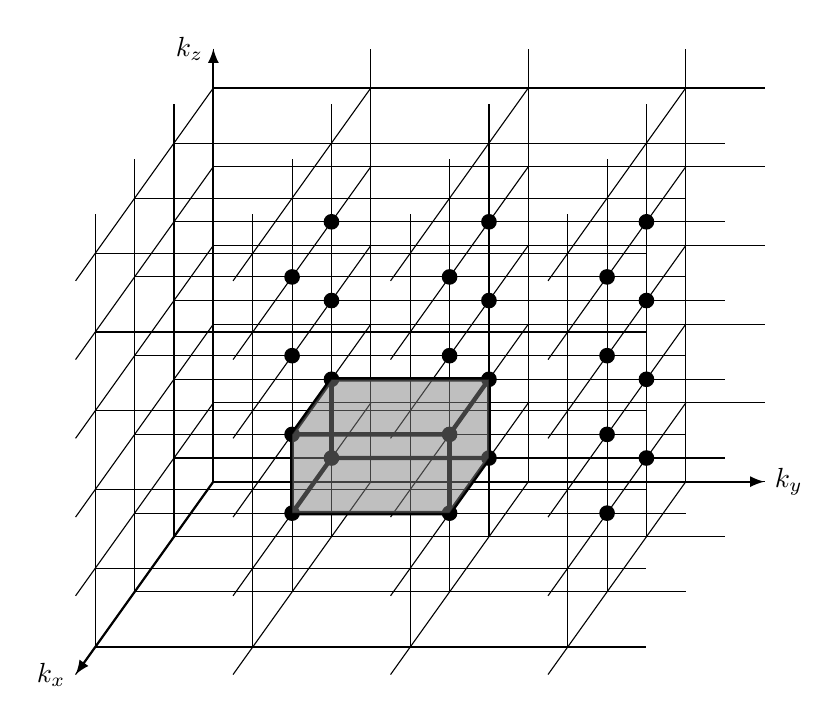
\begin{tikzpicture}[x={(-0.5cm,-0.70cm)}, y={(2cm,0cm)}, z={(0cm,1cm)}]
\draw[-latex, thick] (0,0,0) -- (3.5,0,0) node[left]{$k_x$};
\draw[-latex, thick] (0,0,0) -- (0,3.5,0) node[right]{$k_y$};
\draw[-latex, thick] (0,0,0) -- (0,0,5.5) node[left]{$k_z$};
\foreach \x in {0,1,2,3}{\draw (\x,0,0) -- (\x, 3.5, 0)  (\x,0,1) -- (\x,3.5,1) (\x,0,2) -- (\x,3.5,2)  (\x,0,3) -- (\x,3.5,3)  (\x,0,4) -- (\x,3.5,4) (\x,0,5) -- (\x,3.5,5)  ;}
\foreach \y in {0,1,2,3}{\draw (0,\y,0) -- (3.5, \y, 0)  (0,\y,1) -- (3.5, \y, 1) (0,\y,2) -- (3.5, \y, 2)  (0,\y,3) -- (3.5, \y, 3) (0,\y,4) -- (3.5, \y, 4) (0,\y,5) -- (3.5, \y, 5) ;}
\foreach \x in {0,1,2,3}{\draw (\x,0,0) -- (\x, 0,5.5)   (\x,1,0) -- (\x, 1,5.5)   (\x,2,0) -- (\x, 2,5.5)   (\x,3,0) -- (\x, 3,5.5)  ;}
\draw[ultra thick] (1,1,1) -- (2,1,1) -- (2,2,1) -- (1,2,1) -- (1,1,1);
\draw[ultra thick] (1,1,2) -- (2,1,2) -- (2,2,2) -- (1,2,2) -- (1,1,2);
\draw[ultra thick] (1,1,1) node[circle, fill, inner sep=2pt]{} -- (1,1,2) node[circle, fill, inner sep=2pt]{} (2,1,1) node[circle, fill, inner sep=2pt]{} -- (2,1,2) node[circle, fill, inner sep=2pt]{} (2,2,1) node[circle, fill, inner sep=2pt]{} -- (2,2,2) node[circle, fill, inner sep=2pt]{} (1,2,1) node[circle, fill, inner sep=2pt]{} -- (1,2,2) node[circle, fill, inner sep=2pt]{};
\draw[fill=gray, opacity=0.5] (1,1,2) -- (2,1,2) -- (2,1,1) -- (2,2,1) -- (1,2,1) -- (1,2,2) -- (1,1,2);
\foreach \z in {1,2,3,4} {\draw (1,3,\z) node[circle, fill, inner sep=2pt]{} (2,3,\z) node[circle, fill, inner sep=2pt]{};}
\foreach \z in {3,4} {\draw (1,1,\z) node[circle, fill, inner sep=2pt]{} (2,1,\z) node[circle, fill, inner sep=2pt]{} (1,2,\z) node[circle, fill, inner sep=2pt]{} (2,2,\z) node[circle, fill, inner sep=2pt]{};}
\end{tikzpicture}
\caption{آزاد الیکٹران گیس۔ جال کا ہر نقطہ تقاطع ایک ساکن حال کو ظاہر کرتا ہے۔ ایک "ڈبا" کو سیاہ   دکھایا گیا ہے۔ ایک ڈبہ  کے لئے ایک حال پایا جاتا ہے۔}
\label{شکل_متماثل_ایک_ڈبا_ایک_حال}
\end{figure}

 
اگر آپ ایک تین آبادی فضا کا تصویر کرے جس کے محور \عددی{k_{x}، k_{y} ،k_{z}}  ہو اور جس پر \عددی{k_{x}=(\pi/l_{x})(2\pi/l_{x})(3\pi/l_{x})\dotsc} اور \عددی{k_{y}=(\pi/l_{y})(2\pi/l_{y})(3\pi/l_{y})\dotsc} اور \عددی{k_{z}=(\pi/l_{z})(2\pi/l_{z})(3\pi/l_{z})\dotsc} پر سیدھے سطحیں   پائے  جاتے ہو تب ہر انفرادی نقطہ تقاطع  ،  منفرد یک ذرا ساکن حال دیگا (شکل \حوالہ{شکل_متماثل_ایک_ڈبا_ایک_حال})۔ اس جال میں ہر ایک خانہ لہٰذا ہر ایک حال کی فضا میں درج ذیل حجم گھیرے گا، جہاں  پورے جسم کا حجم ہے۔
 \begin{align}
\frac{\pi^{3}}{l_{x}l_{y}l_{z}}=\frac{\pi^{3}}{V}\end{align}



 %==============
 \begin{figure}
\centering
\begin{tikzpicture}[x={(-0.5cm,-0.5cm)},y={(1cm,0cm)},z={(0cm,1cm)}]
%\pgfmathsetseed{1}
\pgfmathsetmacro{\kr}{2.75}
\pgfmathsetmacro{\krd}{\kr+0.3}
\pgfmathsetmacro{\kphi}{60}
%\pgfmathsetmacro{\ktheta}{45}
%
%axis
\draw[-stealth] (0,0,0)--(3.5,0,0)node[left]{$k_x$};
\draw[-stealth] (0,0,0)--(0,3.5,0)node[below]{$k_y$};
\draw[-stealth] (0,0,0)--(0,0,3.5)node[left]{$k_z$};
% r, phi , theta
\begin{scope}[canvas is xy plane at z=0]
\draw(\kr,0,0) arc (0:90:\kr);
\draw(\krd,0,0) arc (0:90:\krd);
\end{scope}
%
\begin{scope}[canvas is xz plane at y=0]
\draw(\kr,0,0) arc (0:90:\kr);
\draw(\krd,0,0) arc (0:90:\krd);
\end{scope}
%
\begin{scope}[canvas is yz plane at x=0]
\draw(\kr,0,0) arc (0:90:\kr);
\draw(\krd,0,0) arc (0:90:\krd);
\draw[-latex] (0,0,0)node[circle,inner sep=1.5pt,fill=black]{}--++(30:\kr)node[pos=0.5,below]{$k$};
\draw[latex-] (30:\krd)--++(30:0.5)node[right]{$\dif k$};
\end{scope}
\end{tikzpicture}%
\caption{ کروی پوست کا  \عددی{k} فضا میں ایک مثمن۔}
\label{شکل_متماثل_کروی_پوست_مثمن}
\end{figure}

	فرض کریں مادہ کے ایک ٹکڑا میں \عددی{N} جوہر پائے جاتے ہوں اور ہر جوہر اپنے حصہ کے \عددی{q} آزاد الیکٹران دیتا ہو۔ عملاً کسی بھی کلاں بینی جسامت کے چیز کے لئے \عددی{N} کی قیمت بہت بڑی ہوگی جس کی گنتی  ایوگادرو  عدد میں کی  جائے گی جبکہ \عددی{q} ایک چھوٹا عدد مثلاً 1 یا 2 ہوگا۔ اگر الیکٹران بوزان یا قابل ممیز ذرات ہوتے تب وہ زمینی حال \عددی{\psi_{111}} میں سکونیت اختیار کرتے حقیقتاً الیکٹران  متماثل فرمیان ہیں جن پر پالی اصول مناعت کا اطلاق ہوتا ہے لہٰذا کسی بھی حل کی مکین صرف دو الیکٹران ہو سکتے ہیں۔ یہ \عددی{k} فضا میں ایک کرہ کا ایک مثمن رداس \عددی{k_F} تک بھرے گی جس کو اس حقیقت سے تعین کیا جا سکتا ہے کہ الیکٹران کی ہر ایک جوڑی کو \عددی{\frac{\pi^{3}}{V}} حجم درکار ہوگا  (مساوات \حوالہء{5.40})۔

	\begin{align*}
		\frac{1}{8}(\frac{4}{3} \pi k^{3}_F) =  \frac{Nq}{2}(\frac{\pi^3}{V})
	\end{align*}
یوں
\begin{align}
	k_F =(3\rho\pi^{2})^{\frac{1}{3}}
\end{align}
جہاں
\begin{align}
	\rho \equiv \frac{Nq}{V}
\end{align}
آزاد الیکٹران کثافت ہے(آزاد حجم میں الیکٹرانوں کی تعداد)۔

\عددی{k}  فضا میں مکین اور غیر مکین حالات کی سرحد کو \موٹا{فرمی سطح} کہتے ہیں (اسی کی بنا پر  زیرنوشت میں \عددی{F} لکھا گیا)۔ اس سطح پر طاقتی توانائی کو \موٹا{فرمی توانائی} \عددی{E_F} کہتے ہیں۔آزاد الیکٹران گیس کے لئے درج ذیل ہو گا۔
\begin{align}
	E_F = \frac{h^{2}}{2m}(3\rho\pi^{2})^{\frac{2}{3}}
\end{align}
الیکٹران گیس کی کل توانائی کو درج ذیل طریقہ سے حل کیا جا سکتا ہے. ایک خول جس کی موٹائی \عددی{\dif k} شکل  \حوالہ{شکل_متماثل_کروی_پوست_مثمن}  ہو کا حجم
\begin{align*}
	\frac{1}{8}(4\pi k^{2})dk
\end{align*}
لہٰذا اس خول میں الیکٹران حالات کی تعداد درج ذیل ہوگی
\begin{align*}
	\frac{2[(\frac{1}{2})\pi k^{2}\dif k]}{\pi^{3}/V} = \frac{V}{\pi^{2}}k^{2}\dif k
\end{align*}
ان میں سی ہر ایک حال کی توانائی \عددی{\frac{\hslash^{2}k^{2}}{2m}} مساوات \num{5.39} لہٰذا خول کی توانائی
\begin{align}
	dE = \frac{\hslash^{2}k^2}{2m} \frac{V}{\pi^{2}}k^{2}dk
\end{align}
اور کل توانائی درج ذیل ہوگی
\begin{align}
	E_{tot}=\frac{\hslash^{2}V}{2\pi^{2}m}\int_{0}^{k_F}k^{4}dk = \frac{\hslash^{2}k^{5}_F V}{10\pi^{2}m} = \frac{\hslash^{2}(3\pi^{2}Nq)^{\frac{5}{3}}}{10\pi^{2}m}V^{\frac{-2}{3}}
\end{align}
کوانٹم میکانی توانائی کا کردار کچھ ایسا ہی ہے جیسا سادہ گیس میں اندرونی حراری توانائی \عددی{U} کا ہوتا ہے۔ بالخصوص یہ دیواروں پر ایک دباو پیدا کرتا ہے اور اگر ڈبے کے حجم میں \عددی{dV} کا اضافہ ہو تب کل توانائی میں درج ذیل کمی رونما ہوگی
\begin{align*}
	dE_{tot} = -\frac{2}{3}\frac{\hslash^2(3\pi^{2}Nq)^{\frac{5}{3}}}{10\pi^{2}m}V^{\frac{5}{3}}dV = -\frac{2}{3}E_{tot}\frac{dV}{V}
\end{align*}
جو بیرون پر کوانٹم دباو \عددی{P} کا کیا ہوا کام \عددی{dW = PdV} نظر آتا ہے
\begin{align}
	P = \frac{2}{3}\frac{E_{tot}}{V} = \frac{2}{3}\frac{\hslash^{2}k^{5}_F}{10\pi^{2}m} = \frac{(3\pi^{2})^{\frac{2}{3}}\hslash^{2}}{5m}\rho^{\frac{5}{3}}
\end{align}
یہ اس سوال کا جزوی جواب ہے کہ ایک ٹھنڈا ٹھوس جسم اندر کی طرف منہدم کیوں نہیں ہو جاتا۔ ایک اندرونی کوانٹم میکانی دباو توازن برقرار رکھتی ہے جس کا الیکٹران کے  باہمی دفع جنہیں ہم نظر انداز کر چکے ہیں یا حراری حرکت جس کو ہم خارج کر چکے ہیں کے ساتھ کوئی تعلق نہیں ہے۔ بلکہ جو متماثل فرمیان کی ضرورت خلاف تشاکلیت سے پیدا ہوتا ہے۔ اس کو بعض اوقات انحطاطی دباو کہتے ہیں اگرچہ    مناعتی  دباو بہتر اصطلاح ہو گی۔

\ابتدا{سوال}
ایک آزاد الیکٹران کی اوسط توانائی \عددی{\frac{E_{tot}}{Nq}} کو فرمی توانائی کے قصر کی صورت میں لکھیں۔

جواب: \عددی{\frac{3}{5}E_F}
\انتہا{سوال}
\ابتدا{سوال}
تانبا کی کثافت \عددی{\SI{8.96}{\gram \per \centi\meter\cubed}} ہے جبکہ اس کا جوہری وزن \عددی{\SI{63.5}{\gram \per \mole}} ہے۔

(الف) مساوات \عددی{\num{5.43}}استعمال کرتے ہوئے \عددی{q = 1} لیتے ہوئے تانبے کی فرمی توانائی کا حساب لگا کر نتیجہ کو الیکٹران وولٹ کی صورت میں لکھیں۔

(ب) الیکٹران کی مطابقتی سمتی رفتار کیا ہوگی؟اشارہ: \عددی{E_F = (\frac{1}{2})mv^{2}} لیں۔ کیا تانبا  میں الیکٹران کو غیر اضافی تصور کرنا   خطرے  سے باہر ہو گا؟

(ج) تانبا کے لئے کس درجہ حرارت پر امتیازی حراری توانائی \عددی{k_{B}T} جہاں \عددی{k_B} بولٹزمن مستقل اور \عددی{T} کیلون حرارت ہے فرمی توانائی کے برابر ہوگا؟ تبصرہ: اس کو فرمی حرارت کہتے ہیں۔ جب تک حقیقی حرارت فرمی حرارت سے کافی کم ہو مادہ کو ٹھنڈا تصور کیا جا سکتا ہے اور اس میں الیکٹران نچلے ترین قابلِ پہنچ حال میں ہوں گے۔ چونکہ تانبے \عددی{\SI{1356}{\kelvin}} پر پگھلتا  ہے لہٰذا ٹھوس تانبا ہر صورت ٹھنڈا ہوگا۔
 
(د) الیکٹران گیس نمونہ میں تانبا کے لئے انحطاطی دباو مساوات \عددی{\num{5.46}} کا حساب لگائیں۔
\انتہا{سوال}
\ابتدا{سوال}
کسی جسم پر دباو میں معمولی کمی اور نتیجتاً حجم میں نسبتی اضافہ کے تناسب کو جسم مقیاس کہتے ہیں۔
\begin{align*}
	B = -V\frac{dP}{dV}
\end{align*}
دکھائیں کہ آزاد الیکٹران نمونہ میں\عددی{B = \frac{5}{3}P} ہوگا اور سوال\عددی{\num{5.16}(\text{\RL{د}})} کا نتیجہ استعمال کرتے ہوئے تانبا کے لئے جسیم مقیاس کی اندازاً قیمت تلاش کریں۔ تبصرہ: تجربہ سے حاصل قیمت \عددی{\SI{13.4e10}{\newton \per \meter \squared}} ہے مکمل درست جواب کی توقع نہ کریں چونکہ ہم نے الیکٹران مرکزہ اور الیکٹران الیکٹران قوتوں کو نظرانداز کیا ہے! حقیقت میں یہ ایک حیران کن نتیجہ ہے کہ حساب سے حاصل نتیجہ حقیقت کے اتنا قریب ہے۔ 
\انتہا{سوال}

\جزوحصہ{پٹی دار  ساخت}
ہم آزاد الیکٹران نمونہ میں منظم فاصلوں پر ساکن مثبت بار کے مرکزہ کی الیکٹرانوں پر قوت کو شامل کر کے بہتر نمونہ حاصل کرتے ہیں۔ ٹھوس اجسام کا رویہ نمایاں حد تک  اس حقیقت پر مبنی ہے کہ اس کا مخفیہ دوری ہوتا ہے۔ مخفیہ کی حقیقی شکل و صورت مادہ کی تفصیلی رویہ میں کردار ادا کرتی ہے۔ یہ عمل دیکھنے کی خاطر میں سادہ ترین نمونہ تیار کرتا ہوں جس سے یک بُعدی ڈیراک کنگھی کہتے ہیں اور جو ایک جتنے برابر فاصلوں پر نوکیلی ڈیلٹا تفاعلات  پر مشتمل ہوتا ہے (شکل \حوالہ{شکل_متماثل_ڈیراک_کنگھی}) ۔ لیکن اس سے پہلے میں ایک طاقتور مسئلہ پیش کرتا ہوں جو دوری مخفیہ کے مسائل کا حل نہایت سادہ بناتا ہے۔


\begin{figure}
\centering
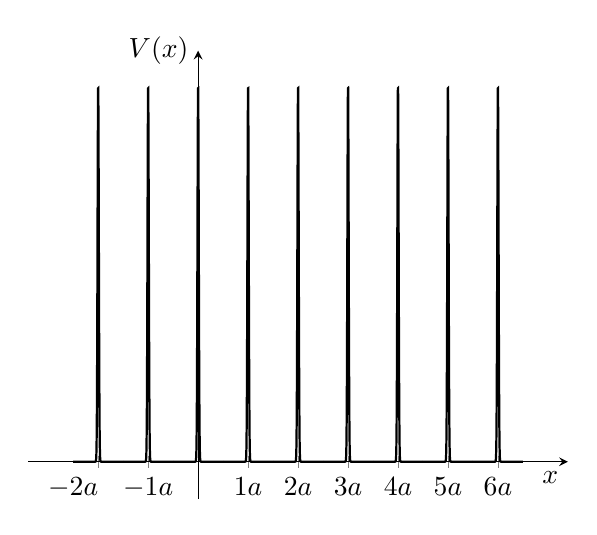
\begin{tikzpicture}
\begin{axis}[axis lines=middle,xlabel={$x$},ylabel={$V(x)$}, xtick={-2,-1,0,1,2,3,4,5,6},
 xticklabels={\llap{$-2a$} ,$-1a$, $0$,  $1a$, $2a$, $3a$, $4a$, $5a$, $6a$}, ytick={\empty}, ylabel style={at={(current axis.above origin)},anchor=east},xlabel style={at={(current axis.right of origin)},anchor=north east},enlargelimits]
\pgfmathsetmacro{\c}{-2}
\addplot [thick,domain=\c-0.5:\c+0.5,samples=200,]	{exp(-3000*(x-\c)^2)};
\pgfmathsetmacro{\c}{-1}
\addplot [thick,domain=\c-0.5:\c+0.5,samples=200,]	{exp(-3000*(x-\c)^2)};
\pgfmathsetmacro{\c}{0}
\addplot [thick,domain=\c-0.5:\c+0.5,samples=200,]	{exp(-3000*(x-\c)^2)};
\pgfmathsetmacro{\c}{1}
\addplot [thick,domain=\c-0.5:\c+0.5,samples=200,]	{exp(-3000*(x-\c)^2)};
\pgfmathsetmacro{\c}{2}
\addplot [thick,domain=\c-0.5:\c+0.5,samples=200,]	{exp(-3000*(x-\c)^2)};
\pgfmathsetmacro{\c}{3}
\addplot [thick,domain=\c-0.5:\c+0.5,samples=200,]	{exp(-3000*(x-\c)^2)};
\pgfmathsetmacro{\c}{4}
\addplot [thick,domain=\c-0.5:\c+0.5,samples=200,]	{exp(-3000*(x-\c)^2)};
\pgfmathsetmacro{\c}{5}
\addplot [thick,domain=\c-0.5:\c+0.5,samples=200,]	{exp(-3000*(x-\c)^2)};
\pgfmathsetmacro{\c}{6}
\addplot [thick,domain=\c-0.5:\c+0.5,samples=200,]	{exp(-3000*(x-\c)^2)};
\end{axis}
\end{tikzpicture}
\caption{ڈیراک کنگھی۔ مساوات \حوالہء{5.57}}
\label{شکل_متماثل_ڈیراک_کنگھی}
\end{figure}



دوری مخفیہ سے مراد ایسا مخفیہ ہے جو کسی مستقل فاصلہ \عددی{a} کے بعد اپنے آپ کو  دہراتا ہے۔  
\begin{align}
	V(x+a) = V(x)
\end{align}
مسئلہ بلوخ کہتا ہے کہ دوری مخفیہ کے لئے مساوات شروڈنگر،
\begin{align}
	-\frac{\hslash^{2}}{2m}\frac{d^{2}\psi}{dx^{2}} +V(x)\psi = E\psi
\end{align}
کے حل سے مراد وہ تفاعل لیا جا سکتا ہے جو درج ذیل شرط کو مطمئن کرتا ہو
\begin{align}
	\psi(x+a) = e^{iKa}\psi(x)
\end{align}
جہاں \عددی{K} ایک مستقل ہے۔ یہاں مستقل سے مراد ایسا تفاعل ہے جو \عددی{x} کا تابع نہیں ہے اگرچہ یہ \عددی{E} کا تابع ہو سکتا ہے۔

\موٹا{ثبوت}: مان لیں کے \عددی{D} ایک ہٹاو عامل ہے:
\begin{align}
	Df(x) = f(x+a)
\end{align}
دوری مخفیہ مساوات \num{5.47} کی صورت میں \عددی{D} ہیملٹنی کا  مقلوبی  ہو گا:
\begin{align}
	[D, H] = 0
\end{align}
لہٰذا ہم \عددی{H} کے ایسے امتیازی تفاعلات چن سکتے ہیں جو بیک وقت \عددی{D} کے امتیازی تفاعلات بھی ہوں:\عددی{D\psi = \lambda\psi} یا
\begin{align}
	\psi(x+a) = \lambda\psi(x)
\end{align}
یہاں \عددی{\lambda} کسی صورت صفر نہیں ہو سکتا اگر یہ صفر ہو تب چونکہ مساوات \num{5.52} تمام \عددی{x} کے لئے مطمئن ہوگا لہٰذا ہمیں \عددی{\psi(x) = 0} ملے گا جو قابلِ قبول امتیازی تفاعل نہیں ہے۔ کسی بھی غیر مخلوط عدد کی طرح اس کو قوت نمائی روپ میں لکھا جا سکتا ہے: 
\begin{align}
	\lambda = e^{iKa}
\end{align}
جہاں \عددی{K} ایک مستقل ہوگا۔

اس مقام پر مساوات \num{5.53} امتیازی قدر \عددی{\lambda} لکھنے کا ایک انوکھا طریقہ ہے لیکن ہم جلد دیکھیں گے کہ \عددی{K} حقیقی ہے اور یوں اگرچہ \عددی{\psi(x)} ازخود غیر دوری ہے\عددی{\abs{\psi(x)}^{2}} جو درج ذیل ہے۔
\begin{align}
	\abs{\psi(x+a)}^{2} = \abs{\psi(x)}^{2}
\end{align}
دوری ہوگا جیسا کہ ہم توقع کرتے ہیں۔


اب ظاہر ہے کہ کوئی بھی  \ترچھا{حقیقی} ٹھوس جسم ہمیشہ کے لئے چلتا نہیں جائے گا بلکہ کہیں نہ کہیں اس کی سرحد پائی جائے گی جو \عددی{V(x)} کی دوریت کو ختم کرتے ہوئے مسئلہ بلوخ کو ناکارہ بنا دے گی۔ تاہم کسی بھی کلاں بین سطح کے  قلم میں کئی ایوگادرو عدد کے برابر جوہر پائے جائیں گے اور ہم فرض کر سکتے ہیں کہ ٹھوس جسم کی سطح سے بہت دور الیکٹران پر سطحی اثر قابل نظر انداز ہوگا۔ ہم مسئلہ بلوخ پر پورا اترنے کی خاطر \عددی{x} کو ایک دائرے پر رکھتے ہیں تاکہ اس کا سر  بہت بڑی تعداد \عددی{N\approx10^{23}} دوری فاصلوں کے بعد اس کے دم  پر پایا جاتا ہو؛  باضابطہ طور پر ہم درج ذیل سرحدی شرط مسلط کرتے ہیں۔   
\begin{align}
	\psi(x+Na) = \psi(x)
\end{align}
یوں مساوات \num{5.49} کے تحت درج ذیل ہوگا
\begin{align*}
	e^{iNKa}\psi(x) = \psi(x)
\end{align*}
لہٰذا \عددی{e^{iNKa} = 1} یا \عددی{NKa = 2\pi n} ہوگا جس کے تحت درج ذیل ہوگا 
\begin{align}
	K = \frac{2\pi n}{Na}, (n = 0, \pm1, \pm2, \dots)
\end{align}
یہاں \عددی{K} لازماً حقیقی ہوگا مسئلہ بلوخ کی افادیت یہ ہے کہ ہمیں صرف ایک خانہ مثلاً \عددی{(0\leq x<a)} کے وقفہ پر مسئلہ شروڈنگر حل کرنا ہوگا مساوات \num{5.49} کی بار بار اطلاق سے ہر جگہ کے حالات  حاصل ہوں گے۔

اب فرض کریں کے مخفیہ در حقیقت نوکیلی ڈیلٹا تفاعلات ڈیراک کنگھی پر مشتمل ہو:
\begin{align}
	V(x) = \alpha\sum_{j=0}^{N-1}\delta(x-ja)
\end{align}
شکل\num{5.5} میں آپ تصور کریں گے  کہ محور \عددی{x} کو یوں دائروی شکل میں  گھمایا گیا ہے کہ \عددی{N}ویں نوکیلی تفاعل درحقیقت نقطہ \عددی{x= -a}  پر پایا جاتا ہے۔ اگرچہ یہ حقیقت پسند نمونہ نہیں ہے لیکن یاد رہے ہمیں دوریت سے دلچسپی ہے۔ کلاسیکی طور پر دہراتا ہوا مستطیلی مخفیہ استعمال کیا گیا جو اب بھی بہت سے مصنفین کا پسندیدہ مخفیہ ہے خطہ \عددی{(0<x<a)} میں مخفیہ صفر ہوگا لہٰذا 
\begin{align*}
	-\frac{\hslash^{2}}{2m}\frac{d^{2}\psi}{dx^{2}} = E\psi,
\end{align*}
یا
\begin{align*}
	\frac{d^{2}\psi}{dx^{2}} = -k^{2}\psi,
\end{align*}
ہوگا۔

جہاں ہمیشہ کہ طرح درج ذیل ہوگا 
\begin{align}
	k = \frac{\sqrt{2mE}}{\hslash},
\end{align}
اس کا عمومی حل درج ذیل ہے 
\begin{align}
	\psi(x) = A\sin(kx) + B\cos(kx), (0<x<a).
\end{align}
مسئلہ بلوخ کے تحت مبدا کے بالکل بائیں ہاتھ پہلے خانہ میں تفاعل موج درج ذیل ہوگا 
\begin{align}
	\psi(x) = e^{-iKa}[A\sin k(x+a) + B\cos k(x+a)], (-a<x<0). 
\end{align}
نقطہ\عددی{x=0} پر \عددی{\psi} لازماً استمراری ہوگا لہٰذا 
\begin{align}
	B = e^{-iKa}[A\sin(ka) + B\cos(ka)];
\end{align}
اس کے تفرق میں ڈیلٹا تفاعل کی زور کے براہ راست متناسب عدم استمرار پائے جائے گی مساوات\num{2.125} جس میں \عددی{\alpha} کی علامت اُلٹ ہوگی چونکہ یہاں کنواں کی بجائے نوکیلی تفاعل پایا جاتا ہے
\begin{align}
	kA - e^{-iKa}k[A\cos(ka) - B\sin(ka)] = \frac{2m\alpha}{\hslash^{2}}B
\end{align}
مساوات \num{5.61} کو \عددی{A\sin(ka)} کے لئے حل کرتے ہوئے درج ذیل حاصل ہوگا 
\begin{align}
	A\sin(ka) = [e^{iKa}-\cos(ka)]B
\end{align}
اس کو مساوات \num{5.62} میں پُر کرتے ہوئے اور \عددی{k_B} کو منسوخ کرتے ہوئے 
\begin{align*}
	[e^{iKa}-\cos(ka)][1-e^{-iKa}\cos(ka)] + e^{-iKa}\sin^{2}(ka) = \frac{2m\alpha}{\hslash^{2}k}\sin(ka)
\end{align*}
حاصل ہوگا۔

جس سے درج ذیل سادہ روپ حاصل ہوتا ہے
\begin{align}
	\cos(Ka) = \cos(ka) + \frac{m\alpha}{\hslash^{2}k}\sin(ka)
\end{align}
یہ ایک بنیادی نتیجہ ہے جس سے باقی سب کچھ اخذ ہوتا ہے۔ کرانگ و  پینی مخفیہ حاشیہ \num{18} دیکھیں کے لئے کلیہ زیادہ پیچیدہ ہوگا لیکن جو خدوخال ہم دیکھنے جا رہے ہیں وہی اس میں بھی پائے جاتے ہیں۔

 مساوات \num{5.64} \عددی{k} کی ممکنات قیمتیں لہٰذا اجازتی توانائیاں تعین کرتی ہیں۔ علامتیت کو سادہ بنانے کی نقطہ نظر سے ہم درج ذیل لکھتے ہیں 
\begin{align}
	z \equiv ka, \text{and} \beta \equiv \frac{m\alpha a}{\hslash^{2}}
\end{align}
جس سے مساوات \num{5.64} کا دایاں ہاتھ درج ذیل روپ اختیار کرتا ہے
\begin{align}
	f(z) \equiv \cos(z) + \beta\frac{\sin(z)}{z}
\end{align}

%figure 5.6 pg 240
\begin{figure}
\centering
\begin{tikzpicture}[declare function={f(\x)=cos(\x) + 10*180/(pi*\x)*sin(\x);}]
%\addplot[domain=130:900,samples=400]{f(x)};
\draw (0,0) node[left]{$0$} -- (9,0) node[right]{$0$};
\draw [name path=xa] (0,1) node[left]{$1$} -- (9,1) node[right]{$1$};
\draw (0,2.75) -- (9,2.75);
\draw (0,-2.75) -- (9,-2.75);
\draw [name path=xb] (0,-1) node[left]{$-1$} -- (9,-1) node[right]{$-1$};
\draw (0,-2.75) node[below]{$0$} -- (0,2.75);
\draw (1.8,-2.75) node[below]{$\pi$} -- (1.8,2.75);
\draw [name path=ya] (3.6,-2.75) node[below]{$2\pi$} -- (3.6,2.75);
\draw [name path=yb] (5.4,-2.75) node[below]{$3\pi$} -- (5.4,2.75);
\draw [name path=yc] (7.2,-2.75) node[below]{$4\pi$} -- (7.2,2.75);
\draw [name path=yd] (9,-2.75) node[below]{$5\pi$} -- (9,2.75);
\draw[thick, domain=130:900,variable=\x,samples=400,name path=f] plot (\x/100,{cos(\x) + 10*180/(pi*\x)*sin(\x)});
\draw [fill=gray, opacity=0.5, name intersections={of={xa and f}}](intersection-1) --++ (0,-2) -- (1.8,-1) -- (1.8,1) -- (intersection-1);
\draw [fill=gray, opacity=0.5, name intersections={of={xb and f}}](intersection-2) --++ (0,2) -- (3.6,1) -- (3.6,-1) -- (intersection-2);
\draw [fill=gray, opacity=0.5, name intersections={of={xa and f}}](intersection-3) --++ (0,-2) -- (5.4,-1) -- (5.4,1) -- (intersection-3);
\draw [fill=gray, opacity=0.5, name intersections={of={xb and f}}](intersection-4) --++ (0,2) -- (7.2,1) -- (7.2,-1) -- (intersection-4);
\draw [fill=gray, opacity=0.5, name intersections={of={xa and f}}](intersection-5) --++ (0,-2) -- (9,-1) -- (9,1) -- (intersection-5);
\end{tikzpicture}
\caption{تفاعل \عددی{f(z)}  (مساوات \حوالہء{5.66})  کو \عددی{\beta=10} کے لئے ترسیم کر کے اجازتی  پٹیاں  (سایہ دار)  دکھائی گئی ہیں  جن کے بیچ  ممنوعہ درز   (جہاں \عددی{\abs{f(z)}>1}  ہو گا)  پائے  جاتے ہیں۔}
\label{شکل_متماثل_اجازتی_ممنوعہ_پٹیاں}
\end{figure}


مستقل \عددی{\beta} بُعدی ہے جو ڈیلٹا تفاعل کی زور کی ناپ ہے شکل  \حوالہ{شکل_متماثل_اجازتی_ممنوعہ_پٹیاں}   میں میں نے \عددی{\beta = 10} کے لئے \عددی{f(z)} کو ترسیم کیا ہے۔ یہاں دیکھنے کی اہم بات یہ ہے کے\عددی{f(z)} ساتھ\عددی{(-1, +1)} سے باہر بھٹکتا ہے اور چونکہ \عددی{\abs{\cos(Ka)}} کی قیمت کسی صورت ایک سے تجاوز نہیں کر سکتی ہے لہٰذا ایسی خطوں میں مساوات \num{5.64} کا حل نہیں پایا جائے گا۔ یہ درز ممنوع توانائیوں کو ظاہر کرتی ہے انکے بیچ اجازتی توانائیوں کی پٹیاں پائی جاتی ہیں مساوات \num{5.56} کے تحت \عددی{Ka = \frac{2\pi n}{N}} ہے جہاں \عددی{N} ایک بہت بڑا عدد ہے لہٰذا \عددی{n} کوئی بھی عدد صحیح ہو سکتا ہے۔ یوں کسی ایک پٹی میں تقریباً ہر توانائی اجازتی ہوگی۔ آپ تصور میں شکل \حوالہ{شکل_متماثل_اجازتی_ممنوعہ_پٹیاں}  پر \عددی{\cos(\frac{2\pi n}{N})} قیمت کے فاصلوں  پر \عددی{+1(n = 0)} سے لے کر نیچے \عددی{-1(n = \frac{N}{2})} تک اور واپس تقریباً \عددی{+1(n = N-1)} تک جہاں بلوخ جزو ضربی \عددی{e^{iKa}} دوبارہ چکر شروع کرتا ہے  لہٰذا \عددی{n} کو مزید بڑھانے سے کوئی نیا حل حاصل نہیں ہو گا لکیریں کھینچ کر دیکھ سکتے ہیں۔ ان لکیروں میں ہر ایک کا \عددی{f(z)} کے ساتھ تقاطع ایک اجازتی توانائی دیگا۔ ظاہر ہے کہ ہر پٹی میں \عددی{N} حالات پائے جاتے ہیں جو ایک دوسرے کے اتنے قریب ہیں  کہ کسی بھی نقطہ نظر سے انہیں ایک مسلسل خطہ تصور کیا جا سکتا ہے (شکل \حوالہ{شکل_متماثل_دوری_مخفیہ_استمراری_پٹیاں})۔

%fig 5.7 pg 240
\begin{figure}
\centering
\begin{tikzpicture}
\pgfmathsetmacro{\a}{1}
\pgfmathsetmacro{\c}{2.5}
\pgfmathsetmacro{\e}{3.9}
\draw[-stealth] (0,0) -- (0,5.5) node[left]{$E$};
\draw[] (0,0) -- (2,0) -- (2,4.5);
\foreach \y in{0,0.05,...,0.70}{\draw[thin](0,\y+\a) -- (2,\y+\a);}
\foreach \y in{0,0.05,...,1}{\draw[thin](0,\y+\c) -- (2,\y+\c);}
\foreach \y in{0,0.05,...,1.25}{\draw[thin](0,\y+\e) -- (2,\y+\e);}
\draw [decorate, decoration={brace,amplitude=5pt,mirror},xshift=4pt] (2,1) -- (2,1.7) node[midway,xshift=15pt]{پٹی};
\draw [decorate, decoration={brace,amplitude=5pt,mirror},xshift=4pt] (2,2.5) -- (2,3.5) node[midway,xshift=15pt]{پٹی};
\draw [decorate, decoration={brace,amplitude=5pt,mirror},xshift=4pt] (2,3.9) -- (2,5.15) node[midway,xshift=15pt]{پٹی};
\draw [decorate, decoration={brace,amplitude=5pt},xshift=-4pt] (0,0) -- (0,1) node[midway,xshift=-15pt]{درز};
\draw [decorate, decoration={brace,amplitude=5pt},xshift=-4pt] (0,1.7) -- (0,2.5) node[midway,xshift=-15pt]{درز};
\draw [decorate, decoration={brace,amplitude=5pt},xshift=-4pt] (0,3.5) -- (0,3.9) node[midway,xshift=-15pt]{درز};
\end{tikzpicture}
\caption{دوری مخفیہ کی اجزاتی توانائیاں  بنیادی طور پر  استمراری پٹیاں پیدا کرتی ہیں۔}
\label{شکل_متماثل_دوری_مخفیہ_استمراری_پٹیاں}
\end{figure}

 ہم نے ابھی تک اپنے مخفیہ میں ایک الیکٹران رکھا ہے۔ حقیقت میں \عددی{N_q} الیکٹران ہوں گے جہاں ہر ایک جوہر \عددی{q} تعداد کے آزاد الیکٹران مہیا  کرے گا۔ پالی اصول مناعت کے بنا صرف دو الیکٹران کسی ایک فضائی حال کے مکین ہو سکتے ہیں۔ یوں  \عددی{q = 1} کی صورت میں یہ زمینی حال میں پہلی پٹی کو آدھا   بھریں گے اگر  \عددی{q = 2} ہو تب یہ پہلی پٹی کو مکمل کریں گے اگر \عددی{q = 3} ہو یہ دوسری پٹی کو آدھا بھریں گے وغیرہ وغیرہ. تین ابعاد میں اور زیادہ حقیقی مخفیہ کی صورت میں پٹیوں کی ساخت زیادہ پیچیدہ ہو سکتی ہے لیکن اجازتی پٹیاں جن کے بیچ ممنوع درز پائے جاتے ہوں تب بھی ہوگا۔ دوری مخفیہ کی نشانی بھی پٹی ہے۔
 
 اب اگر ایک پٹی مکمل طور پر بھری ہوئی ہو ممنوع خطہ سے گزرتے ہوئے اگلی پٹی تک چھلانگ کے لئے ایک الیکٹران کو نسبتاً زیادہ توانائی درکار ہوگی ایسا مادہ برقی طور پر غیر موصل ہوگا۔ اس کے برعکس اگر ایک پٹی پوری طرح بھری ہوئی نہیں ہے تب ایک الیکٹران کو بہت معمولی توانائی درکار ہوگی کہ وہ ہیجان ہو سکے  اس طرح کا مادہ عموماً موصل ہوگا۔ ایک غیر موصل میں بڑے یا کم \عددی{q} کے چند جوہر کی ملاوٹ سے اگلی بلند پٹی میں چند اضافی الیکٹران رکھ دیے جاتے ہیں پہلے سے مکمل پُر پٹی میں خول پیدا کیے جاتے ہیں۔ ان دونوں صورتوں میں ایک کمزور برقی رو گزر سکتا ہے اور ایسے اشیاء نیم موصل کہلاتے ہیں۔ آزاد الیکٹران نمونہ میں تمام ٹھوس اجسام کو لازماً بہت اچھا موصل ہونا چاہئے تھا چونکہ انکے اجازتی توانائیوں کے طیف میں کوئی بڑا وقفہ نہیں پایا جاتا ہے۔ قدرت میں پائے جانے والے ٹھوس اجسام کی برقی موصلیت میں اتنا زیادہ فرق صرف نظریہ پٹی کی مدد سے سمجھا سکتا ہے۔  
%==========================

\ابتدا{سوال}

(الف) مساوات \num{5.59} اور مساوات \num{5.63} استعمال کرتے ہوئے دکھائیں کہ دوری ڈیلٹا تفاعل مخفیہ میں ایک ذرے کی تفاعل موج درج ذیل روپ میں لکھی جا سکتی ہے 
\begin{align*}
	\psi(x) = C[\sin(kx)+e^{-iKa}\sin k(a-x)], (0\leq x\leq a).
\end{align*} 
معمول زنی مستقل \عددی{C} تعین کرنے کی ضرورت نہیں ہے۔

(ب)  البتہ پٹی کے بالائی سر پر جہاں \عددی{z} \عددی{\pi} کا عدد صحیح مضرب ہوگا شکل \num{5.6} (الف) سے \عددی{\psi(x) = 0} حاصل ہوگا ایسی صورت میں درست تفاعل موج تلاش کریں دیکھیئے گا کہ ہر ایک ڈیلٹا تفاعل پر \عددی{\psi} کو کیا ہوتا ہے؟
\انتہا{سوال}
\ابتدا{سوال}
پہلی اجازتی پٹی کے نچلے نقطہ پر \عددی{\beta = 10} کی صورت میں توانائی کی قیمت تین با معنی ہندسوں تک تلاش کریں۔ دلائل پیش کرتے ہوئے آپ فرض کر سکتے ہیں کہ\عددی{\frac{\alpha}{a} = \SI{1}{\electronvolt}} ہو گا۔
\انتہا{سوال}
\ابتدا{سوال}
فرض کریں ہم ڈیلٹا تفاعل سوزن کے بجائے ڈیلٹا تفاعل کنواں پر غور کر رہے ہیں یعنی مساوات \num{5.57} میں \عددی{\alpha} کی علامت تبدیل کریں۔ ایسی صورت میں شکل \num{5.6} اور \num{5.7} کی طرح کے اشکال بنائیں۔ مثبت توانائی حلوں کے لئے آپ کو کوئی نیا حساب کرنے کی ضرورت نہیں ہے بس مساوات \num{5.66} میں موضوع تبدیلیاں لائیں لیکن منفی توانائی حلوں کے لئے آپ کو کام کرنا ہوگا اور انہیں ترسیم پر شامل کرنا مت بھولیے گا جو اب \عددی{-z} تک وسیع ہوگا۔ پہلی اجازتی پٹی میں اب کتنے حالات ہونگے؟
\انتہا{سوال}
\ابتدا{سوال}
دکھائیں کہ مساوات \num{5.64} میں حاصل زیادہ تر توانائیاں دوہری انحطاطی ہے۔ کن صورتوں میں ایسا نہیں ہے؟ اشارہ: \عددی{(N=1, 2, 3, 4, \dots)} لیتے ہوئے دیکھیے گا کیا ہوتا ہے۔ ایسی ہر صورت میں \عددی{\cos(Ka)} کی کیا  ممکنہ قیمتیں ہوں گی؟
\انتہا{سوال}

\حصہ{کوانٹم شماریاتی میکانیات}
مطلق صفر حرارت پر ایک طبی نظام اپنے کم سے کم اجازتی توانائی  تشکیل کا مکین ہوگا۔ درجہ حرارت بڑھاتے ہوئے بلا منصوبہ حراری سرگرمیوں کے بنا ہیجانی حالات ابھرنے شروع ہونگے جس سے درج ذیل سوال پیدا ہوتا ہے: اگر \عددی{T} درجہ حرارت پر حراری توازن میں ایک بڑی تعداد \عددی{N} کے ذرات پائے جاتے ہوں تب اس کا کیا احتمال ہے کہ ایک ذروی جس کو بلا منصوبہ منتخب کیا گیا ہو کی مخصوص توانائی \عددی{E_j}؟ ہوگی دھیان رہے کہ اس احتمال کا کوانٹم عدم تعین کے ساتھ کوئی تعلق نہیں ہے بالکل یہی سوال کلاسیکی شماریاتی میکانیات میں بھی کھڑا ہوتا ہے۔ ہمیں احتمالی جواب اس لئے منظور ہوگا کہ جن ذرات کی ہم بات کر رہے ہیں انکی تعداد اتنی بڑی ہوگی کہ یہ کسی صورت ممکن نہیں ہوگا کہ ہم ہر ایک پر علیحدہ علیحدہ نظر رکھ سکیں چاہے یہ قابلِ تعین ہو یا نہ ہوں۔

شماریاتی میکانیات کا بنیادی مفروضہ یہ ہے کہ حراری توازن میں ہر وہ منفرد حال جس کی ایک جیسی کل توانائی \عددی{E} ہو ایک جتنا محتمل ہوگا۔ بلا واسطہ حراری حرکت کی بنا مستقل طور پر توانائی ایک ذروی سے دوسرا ذرہ ایک روپ حرکی، گردشی، گھومتی وغیرہ سے دوسری روپ میں منتقل ہوگی لیکن بیرونی مداخلت کی عدم موجودگی میں بقا  توانائی کی بنا کل مقررہ ہوگا۔ یہاں مفروضہ یہ ہے  کہ توانائی کی لگاتار نئی تقسیم کسی مخصوص حال کو ترجیح نہیں دیتا ہے۔ یہ ایک گہرا مفروضہ ہے جو سوچنے کے قابل ہے درجہ حرارت \عددی{T} حراری توازن میں ایک نظام کی کل توانائی کی بس پیمائش ہے۔ ان منفرد حالات کی گنتی میں کوانٹم میکانیات ایک نئی پیچیدگی پیدا کرتی ہے لیکن چونکہ حالات غیر مسلسل ہیں لہٰذا یہ کلاسیکی نظریہ سے زیادہ آسان ہے اور اس کا فیصلہ کن انحصار اس بات پر ہوگا کہ یہ ذرات قابلِ ممیز، متماثل بوزان یا متماثل فرمیان ہیں۔ ان کے دلائل نسبتاً سیدھے لیکن ریاضی کافی گہری ہے لہٰذا میں ایک انتہائی سادہ  مثال سے شروع کروں گا تاکہ آپ بنیادی حقائق سمجھ سکیں۔
\جزوحصہ{ایک مثال} 
فرض کریں ہمارے پاس یک بعدی لامتناہی چکور کنواں حصہ\num{2.2} میں کمیت \عددی{m} کے صرف تین باہم غیر متعامل ذرات پائے جاتے ہیں۔ ان کی کل توانائی درج ذیل ہوگی مساوات \num{2.27} دیکھیں
\begin{align}
	E = E_A + E_B + E_C = \frac{\pi^2 \hslash ^2}{2ma^2}(n^2_A + n^2_B + n^2_C)
\end{align}
جہاں \عددی{n_A}، \عددی{n_B} اور \عددی{n_C} مثبت عدد صحیح ہوں گے۔ اب تبصرہ جاری رکھنے کی خاطر فرض کریں کہ\عددی{E=363(\frac{\pi ^2 \hslash ^2}{2ma^2})} یعنی درج ذیل
\begin{align}
	n^2_A + n^2_B + n^2_C = 363.
\end{align}  
جیسے آپ تصدیق کر سکتے ہیں ہمارے پاس تین مثبت عدد صحیح اعداد کے تیرہ  ایسے ملاپ  پائے جاتے ہیں جن کے مربعوں کا مجموعہ \num{363} ہوگا: تینوں اعداد گیارہ ہو سکتے ہیں دو اعداد تیرہ  اور ایک پانچ جو تین مرتب اجتماعات میں ہوگا ایک عدد اُٗنّیس اور دو ایک یہاں نھی تین مرتب اجتماعات میں یا ایک عدد سترہ ایک ساٹھ اعر ایک پانچ چھ مرتب اجتماعات میں ہو سکتے ہیں۔ یوں \عددی{n_A, n_B, n_C}  درج ذیل میں سے ایک ہوگا:
\begin{align*}
	(11, 11, 11)\\
	(13, 13, 5), (13, 5, 13), (5, 13, 13)\\
	(1, 1, 19), (1, 19, 1), (19, 1, 1)\\
	(5, 7, 17), (5, 17, 7), (7, 5, 17), (7, 17, 5), (17, 5, 7), (17, 7, 5).
\end{align*}
اگر یہ ذرات قابلِ ممیز ہوں تب ان میں سے ہر ایک کسی ایک منفرد کوانٹم حال کو ظاہر کرے گا اور شماریاتی میکانیات کے بنیادی مفروضہ کے تحت حراری توازن میں یہ سب برابر محتمل ہوں گے۔ لیکن میں اس میں دلچسپی نہیں رکھتا ہوں کہ کونسا ذرہ کس یک ذروی حال میں پایا جاتا ہے بلکہ میں یہ جاننا چاہتا ہوں کہ ہر ایک حال میں کل کتنے ذرات پائے جاتے ہیں حال\عددی{\psi_n} کی تعداد مکین \عددی{N_n}۔ ہم اس دن ذرہ حال کے تمام تعداد مکین کے اجتماع  کو تشکیل  کہتے ہیں۔ اگر تینوں حال \عددی{\psi_{11}}  میں ہوں تب تشکیل  درج ذیل ہوگا
\begin{align}
	(0, 0, 0, 0, 0, 0, 0, 0, 0, 0, 3, 0, 0, 0, 0, 0, 0, 0, \dots)
\end{align} 
یعنی \عددی{N_{11}=3} باقی تمام صفر اگر دو حال \عددی{\psi_{13}} میں اور ایک \عددی{\psi_5} میں ہو تب تشکیل  درج ذیل ہوگا
\begin{align}
	(0, 0, 0, 0, 1, 0, 0, 0, 0, 0, 0, 0, 2, 0, 0, 0, 0, \dots)
\end{align}  
یعنی \عددی{N_5=1, N_{13}=2} باقی تمام صفر اگر دو \عددی{\psi_1} میں ایک \عددی{\psi_{19}} میں تب تشکیل  درج ذیل ہوگا
\begin{align}
	(2, 0, 0, 0, 0, 0, 0, 0, 0, 0, 0, 0, 0, 0, 0, 0, 0, 0, 1, 0, \dots)
\end{align} 
یعنی\عددی{N_1 = 2, N_{19} = 1} باقی تمام صفر اور اگر ایک ذروی \عددی{\psi_5} میں ایک \عددی{\psi_7} میں اور ایک \عددی{\psi_{17}} میں تب تشکیل  درج ذیل ہوگا 
\begin{align}
	(0, 0, 0, 0, 1, 0, 1, 0, 0, 0, 0, 0, 0, 0, 0, 0, 1, 0, 0, \dots)
\end{align} 
یعنی \عددی{N_5 = N_7 = N_{17} = 1, \text{\RL{باقی تمام صفر}}} ان تمام میں آخری تشکیل  زیادہ سے زیادہ محتمل ہوگی چونکہ اسکو چھ مختلف طریقوں سے حاصل کیا جا سکتا ہے جبکہ درمیانی دو کو تین طریقوں سے اور پہلی کو صرف ایک طریقہ سے حاصل کیا جا سکتا ہے۔

میں اب دوبارہ اپنے اصل سوال پر آتا ہوں کہ بلا واسطہ تین ذرات منتخب کرتے ہوئے کوئی مخصوص اجازتی توانائی \عددی{E_n} حاصل کرنے کا احتمال \عددی{P_n} کیا ہوگا؟ توانائی \عددی{E_1} صرف اس صورت حاصل ہوگا جب ذرہ تیسری تشکیل مساوات \num{5.71} میں ہو اس تشکیل میں نظام ہونے کا اتفاق تیرہ میں سے تین ہے اور اس تشکیل میں \عددی{E_1} کے حصول کا احتمال \عددی{\frac{2}{3}} لہٰذا\عددی{P_1 =(\frac{3}{13})\times (\frac{2}{3})= \frac{2}{13}}۔ آپ \عددی{E_5} کو تشکیل دو مساوات \num{5.70} تیرہ میں سے تین کا امکان جس کا احتمال \عددی{\frac{1}{3}} 	یا تشکیل چار مساوات \num{5.72} تیرہ میں سے چھ امکان اور احتمال \عددی{\frac{1}{3}} لہٰذا\عددی{P_5 = (\frac{3}{13})\times(\frac{1}{3}) + (\frac{6}{13})\times(\frac{1}{3}) = \frac{3}{13}}۔ آپ \عددی{E_7} کو صرف چار سے حاصل کر سکتے ہیں لہٰذا\عددی{P_7 = (\frac{6}{13})\times(\frac{1}{3}) = \frac{2}{13}}۔ اسی طرح \عددی{E_{11}} صرف پہلی تشکیل سے مساوات \num{5.69} سے تیرہ میں سے ایک امکان اور احتمال ایک کے ساتھ حاصل ہوگا لہٰذا\عددی{P_{11} = (\frac{1}{13})} ہوگا۔ اسی طرح \عددی{P_{13} = (\frac{3}{13})\times(\frac{2}{3}) =\frac{2}{13}}، \عددی{P_{17} = (\frac{6}{13})\times(\frac{1}{3}) = \frac{2}{13}} اور \عددی{P_{19} = (\frac{3}{13})\times(\frac{1}{3}) = \frac{1}{13}} ہوگا۔ انکی تصدیق درج ذیل سے ہوگی 
\begin{align*}
	P_1 + P_5 + P_7 + P_{11} + P_{13} + P_{17} + P_{19} = \frac{2}{13} + \frac{3}{13} + \frac{2}{13} + \frac{1}{13} + \frac{2}{13} + \frac{2}{13} + \frac{1}{13} = 1.
\end{align*} 

یہ قابلِ ممیز ذرات کے لئے تھا۔ اس کی بجائے اگر ذرات متماثل فرمیان ہوتے اپنی آسانی کے لئے چکر کو  نظرانداز کرتے ہوئے یا اگر آپ چاہیں تو یہ تصور کرتے ہوئے کہ تمام ایک جیسے چکر حال میں ہیں ضرورت خلاف تشاکلیت کی بنا پہلی تین تشکیلات  جو دو یا اس سے بھی برا تین ذرات کے ایک ہی حال میں ڈالتے ہیں خارج امکان ہوں گے لہٰذا چوتھی تشکیل میں صرف ایک حال ہوگا سوال \num{5.22} الف دیکھیں۔ متماثل فرمیان کے لئے \عددی{P_5 = P_7 = P_{17} = \frac{1}{3}} ہوگا اور اب بھی احتمالات کا مجموعہ ایک ہے اس کے برعکس اگر ذرات متماثل بوزان ہوتے تب ضرورت تشاکلیت ہر تشکیل میں صرف ایک حال کی اجازت دیتا سوال \num{5.22} ب دیکھیں۔ لہٰذا\عددی{P_1 = (\frac{1}{4})\times(\frac{2}{3}) = \frac{1}{6}}، \عددی{P_5 = (\frac{1}{4})\times(\frac{1}{3}) + (\frac{1}{4})\times(\frac{1}{3}) = \frac{1}{6}}، \عددی{P_7 = (\frac{1}{4})\times(\frac{1}{3}) = \frac{1}{12}}، \عددی{P_{11} = (\frac{1}{4})\times(1) = \frac{1}{4}}،\عددی{P_{13} = (\frac{1}{4})\times(\frac{2}{3}) = \frac{1}{6}}، \عددی{P_{17} = (\frac{1}{4})\times(\frac{1}{3}) = \frac{1}{12}} اور \عددی{P_{19} = (\frac{1}{4})\times(\frac{1}{3}) = \frac{1}{12}} ہوتا۔ ہمیشہ کی طرح احتمالات کا مجموعہ ایک ہے۔

اس مثال کا مقصد آپ کو یہ دکھانا تھا کہ ذرات کی قسم پر حالات کی شمار کس طرح منحصر ہے۔ ایک لحاظ سے ایک حقیقی صورت حال سے جہاں \عددی{N} ایک بہت بڑا عدد ہوگا سے یہ مثال زیادہ پیچیدہ تھا۔ چونکہ \عددی{N} کی قیمت بڑھانے سے زیادہ محتمل تقسیم جو قابلِ ممیز ذرات کے لئے اس مثال میں \عددی{N_5 = N_7 = N_{17} = 1} ہے پائے جانے کا امکان اتنا زیادہ ہو جائے گا کہ کسی بھی شماریاتی نقطہ نظر سے باقی تمام امکانات کو رد کیا جا سکتا ہے۔ توازن کی صورت میں انفرادی ذرہ توانائیوں کی تقسیم درحقیقت انکی زیادہ سے زیادہ محتمل تشکیل میں تقسیم ہے۔ اگر یہ \عددی{N = 3}  کے لئے درست ہوتا جو کہ یہ نہیں ہے ہم قابلِ ممیز ذرات کے لئے \عددی{N = 3} کی صورت  میں اخذ کرتے \عددی{P_5 = P_7 = P_{17} = \frac{1}{3}} میں حصہ 5.4.3 میں اس نقطہ پر دوبارہ  آوں گا لیکن اس سے پہلے گنتی کی ترکیب کو عمومیت دیتے ہیں۔

\ابتدا{سوال}

(الف) حال \عددی{\psi_5} میں ایک حال \عددی{\psi_7} میں ایک اور حال \عددی{\psi_{17}} میں ایک متماثل تین فرمیان کا مکمل خلاف تشاکل تفاعل موج \عددی{\psi(x_A, x_B, x_C)} تیار کریں۔

(ب) تین متماثل بوزان کے لئے مکمل تشاکل تفاعل موج\عددی{\psi(x_A, x_B, x_C)} درج ذیل صورتوں میں تیار کریں (ا) تینوں حال \عددی{\psi_{11}} میں ہوں، (ب) اگر دو \عددی{\psi_1} اور ایک \عددی{\psi_{19}} میں ہو، (ج) اگر ایک حال \عددی{\psi_5} ایک حال \عددی{\psi_7} اور ایک حال \عددی{\psi_{17}} میں ہو۔ 
\انتہا{سوال}
\ابتدا{سوال}
فرض کریں یک بُعدی ہارمونی ارتعاشی مخفیہ میں آپ کے پاس تین باہم غیر متعامل ذرات ہیں جو حراری توازن میں پائے جاتے ہیں جن کی کل توانائی\عددی{E = (\frac{9}{2})\hslash\omega} ہے۔

(الف) اگر یہ تمام ایک جیسی کمیت کے قابل ممیز ذرات ہوں تب انکی کتنی عدد مکین تشکیلات  ہوں گے اور ہر ایک کے لئے کتنے منفرد تین ذرہ حالات ہوں گے؟ سب سے زیادہ محتمل تشکیل کیا ہوگی؟ اگر آپ ایک ذروی بلا منصوبہ منتخب کریں اور اسکی توانائی کی پیمائش کریں تب کیا قیمتیں متوقع ہوں گی؟ اور ہر ایک کا احتمال کیا ہوگا؟ سب سے زیادہ محتمل توانائی کیا ہوگی؟

(ب) یہی کچھ متماثل فرمیان کے لئے کریں چکر کو نظر انداز کریں جیسا ہم نے حصہ 5.4.1 میں کیا۔

(ج) یہی کچھ متماثل بوزان کے لئے کریں چکر کو نظرانداز کریں۔ 
\انتہا{سوال}
%==============
%the above is prob 5.23 

\جزوحصہ{عمومی صورت}
آئیں اب ایک ایسی مخفیہ پر غور کریں جس کی یک ذرا توانائیاں \عددی{E_1} \عددی{E_2} \عددی{E_3} \عددی{، \dotsc ،} انحطاط \عددی{d_1} \عددی{d_2} \عددی{d_3} \عددی{، \dotsc ،} ہوں یعنی اس میں یک زریں حالات کے تعداد \عددی{d_n} جن کی توانائیاں \عددی{E_n} ہیں فرض کریں ہم کمیت \عددی{m} کے \عددی{N} ذرات کو اس ‏مخفیہ میں رکھتے ہیں ہم تشکیل \عددی{N_1} \عددی{N_2} \عددی{N_3} \عددی{\dotsc} میں دلچسپی رکھتے ہیں جہاں \عددی{N_1} ذرات کی توانائی \عددی{E_1} \عددی{N_2} ذرات کی توانائی \عددی{E_2} وغیرہ وغیرہ ہے سوال ایسا کتنے مختلف طریقوں سے کیا جا سکتا ہے بلکہ یہ کہنا زیادہ درست ہوگا کہ اس مخصوص تشکیل کی مطابقتی کتنے منفرد حالات ہونگے اس کا جواب \عددی{Q(N_1, N_2, N_3, \dotsc)} اس بات پر منحصر ہوگا کہ آیا ذرات قابل ممیز متماثل فرميان یا متماثل بوزان ہے لہٰذا ہم ان تینوں صورتوں پر علیحدہ علیحدہ غور کرتے ہیں ہم پہلے یہ فرض کرتے ہیں کہ ذرات قابل ممیز ہیں دستیاب \عددی{ N} ذرات میں سے کتنے طریقوں سے \عددی{N_1} کو منتخب کر کے پہلا  ٹوکرا میں رکھا جا سکتا ہے جواب: ثنائی عددی سر \عددی{N_1} کو \عددی{ N} میں سے منتخب کرتا ہے 
\begin{align}
\begin{pmatrix}
N \\
N_1
\end{pmatrix}
\equiv \frac{N!}{N_1 ! (N - N_1) !}
\end{align}
پہلا ذرہ \عددی{ N} مختلف طریقوں سے منتخب کیا جا سکتا ہے جس کے بعد \عددی{(N - 1)} ذرات رہ جاتے ہیں لہٰذا دوسرے ذرے کے انتخاب کے \عددی{N - 1} مختلف طریقے ہوں گے وغیرہ وغیرہ 
\begin{align*}
N(N - 1) (N - 2) \dotsc (N - N_1 + 1) = \frac{N !}{(N - N_1) !}
\end{align*}
لیکن یہ \عددی{N_1} ذرات کے \عددی{N_1 !} مختلف مرتب اجتماعات کو علیحدہ علیحدہ گنتا  ہے جبکہ ہمیں اس سے کوئی دلچسپی نہیں کے عدد \عددی{37} کو پہلی انتخاب میں یا \عددی{29} ویں انتخاب میں منتخب کیا گیا لہٰذا ہم \عددی{N_1 !} سے تقسیم کرتے ہیں جس سے مساوات 5.73 حاصل ہوتا ہے اب پہلی ٹوکرا میں ان \عددی{N_1} ذرات کو کتنی مختلف طریقوں سے رکھا جا سکتا ہے چونکہ پہلے ٹوکرا میں \عددی{d_1} حالات ہیں لہٰذا ہر ایک ذروی کو \عددی{d_1} مختلف طریقوں سے چنا جا سکتا ہے یوں ظاہر ہے کہ کل ممکنات \عددی{(d_1)^{N_1}} ہونگے اس طرح ایک ٹوکرا جس میں \عددی{d_1} منفرد متبادل ہوں میں کل آبادی \عددی{N} میں سے \عددی{N_1} ذرات منتخب کر کے رکھنے کے درج ذیل طریقے ہونگے 
\begin{align*}
\frac{N ! d_1^{N_1}}{N_1 ! (N - N_1) !}
\end{align*}
دوسرے ٹوکرے میں صرف \عددی{(N - N_1)} ذرات ہونے کے علاوہ بالکل ایسا ہی ہوگا 
\begin{align*}
\frac{(N - N_1) ! d_2^{N_2}}{N_2 ! (N - N_1 - N_2) !}
\end{align*}
وغیرہ وغیرہ اس طرح درج ذیل ہوگا 
\begin{align}
Q (N_1 , &N_2 , N_3 , \dotsc) \\
&= \frac{N ! d_1^{N_1}}{N_1 ! (N - N_1) !} \frac{(N - N_1) ! d_2^{N_2}}{N_2 ! (N - N_1 - N_2) !} \frac{(N - N_1 - N_2) ! d_3^{N_3}}{N_3 ! (N - N_1 - N_2 - N_3) !} \dotsc\\
&= N ! \frac{d_1^{N_1} d_2^{N_2} d_3^{N_3} \dotsc}{N_1 ! N_2 ! N_3 ! \dotsc} = N! \prod_{n = 1}^{infty} \frac{d_n^{N_n}}{N_n !}
\end{align}
یہاں رک کر اس نتیجہ کی تصدیق کیجیے گا مثال کے طور پر حصہ 5.4.1 میں سوال 5.24 دیکھیں متماثل فرمیان کے لئے یہ مسئلہ نسبتاً بہت آسان ہے چونکہ یہ غیر ممیز ہیں لہٰذا اس سے کوئی فرق نہیں پڑتا کے کونسا ذرا کس حال میں ہے ضرورت خلاف تشاکلیت کے تحت ایک مخصوص ایک ذروی حالات کے سلسلہ کو بھرنے کے لئے صرف ایک \عددی{ N } ذرا حال ہوگا مزید واحد ایک ذروی کسی ایک حال کو بھر سکتا ہے لہٰذا \عددی{ N} ویں ٹوکرا میں \عددی{N_n} بهرے  حالات کو منتخب کرنے کے 
\begin{align*}
\begin{pmatrix}
d_n \\
N_n
\end{pmatrix}
\end{align*}
طریقے ہونگے اس طرح درج ذیل ہوگا 
\begin{align}
Q (N_1 , N_2 , N_3 , \dotsc ) = \prod_{n = 1}^{\infty} \frac{\dif_n !}{N_n ! (\dif_n - N_n) !}
\end{align}
اس کی تصدیق کیجیے گا مثلاً حصہ 5.4.1 میں سوال 5.24 دیکھ کر متماثل بوزان کے لیے یہ حساب سب سے مشکل ہوگا یہاں ضرورت تشاکلیت کے تحت ایک ذروی حالات کہ ایک مخصوص سلسلہ کو بھرنے کا صرف ایک \عددی{N} ذرہ حال ہوگا تاہم یہاں اس ایک ذروی حال کو بھرنے پر ذرات کی تعداد پر پابندی عائد نہیں ہوگی یہاں \عددی{N} وی ٹوکرے کیلئے سوال یہ ہوگا ہم متماثل \عددی{N_n} ذرات کو \عددی{d_n} مختلف خانوں میں کس طرح رکھ سکتے ہیں غیر مرتب اجتماعات کے سوال کو حل کرنے کے کئی طریقے ہیں ایک دلچسپ طریقہ درج ذیل ہے ہم ذرا کو نقطہ اور خانوں کو صلیب سے ظاہر کرتے ہیں یوں مثال کے طور پر \عددی{d_n = 5} اور \عددی{N_n = 7} کی صورت میں
\begin{align*} 
\bullet \quad \bullet \quad \times \quad \bullet \quad \times \quad \bullet \quad \bullet \quad \bullet \quad \times \quad \bullet \quad \times
\end{align*}
یہ ظاہر کرے گا کہ پہلے حال میں دو ذرات دوسرے حال میں ایک ذروی تیسرے میں تین چوتھے میں ایک اور پانچویں میں کوئی ذرا نہیں پایا جاتا ہے دھیان رہے کہ نقطوں کی تعداد \عددی{N_n} اور صلیبوں کی تعداد \عددی{d_n - 1} ہیں جو ان نقطوں کو \عددی{d_n} گروہ میں خانہ بند کرتے ہیں اگر ان انفرادی نقطوں اور صلیبوں کو نام دیے جاتے تب انہیں \عددی{(N_n + d_n - 1) !} مختلف طریقوں سے رکھا جا سکتا تھا تاہم ہمارے لئے تمام نقطے ایک دوسرے  جیسے ہیں اور ان کو \عددی{N_n !} مختلف مرتب اجتماعات کی صورت میں لکھنے سے حال تبدیل نہیں ہوتا اسی طرح تمام صلیب معطل ہیں اور انہیں \عددی{(d_n - 1) !} مختلف مرتب اجتماعات لکھنے سے کچھ بھی تبدیل نہیں ہوگا یوں \عددی{N} وی ٹوکرا میں \عددی{d_n} یک ذروی حالات کو \عددی{N_n} ذرات مختص کرنے کے درج ذیل منفرد طریقے ہونگے 
\begin{align}
\frac{(N_n + d_n - 1) !}{N_n ! (d_n - 1) !} = 
\begin{pmatrix}
N_n + d_n - 1 \\
N_n
\end{pmatrix}
\end{align}
جس کی بنا ہم درج ذیل اخذ کرتے ہیں 
\begin{align}
Q(N_1 , N_2 , N_3 , \dotsc) = \prod_{n = 1}^{\infty} \frac{(N_n + d_n - 1) !}{N_n ! (d_n - 1) !}
\end{align}
اس کی تصدیق کیجیے گا مثلاً حصہ 5.4.1 میں سوال 5.24 کے ساتھ 


\ابتدا{سوال}
حصہ 5.4.1 میں مثال کے ساتھ مساوات 5.74 5.75 اور 5.77 کی تصدیق کیجیے گا 
\انتہا{سوال}
\ابتدا{سوال}
مساوات 5.76 کو الكراجى ماخوذ کی مدد سے حاصل کریں غیر مرتب اجتماعات کا سوال درج ذیل ہوگا آپ \عددی{d} ٹوکریوں میں \عددی{N} متماثل گیندوں کو کتنے مختلف طریقوں سے رکھ سکتے ہیں اس سوال کی نقطہ نظر سے زیرنوشت میں ان کو نظر انداز کریں آپ تمام کے تمام \عددی{N} کو تیسری ٹوکری میں یا ایک کو پانچویں اور باقیوں کو دوسری ٹوکری میں یا تو کو پہلی اور تین کو تیسری ٹوکری میں اور باقی کو ساتویں ٹوکری میں وغیرہ وغیرہ رکھ سکتے ہیں اس کو صریحاً \عددی{N = 1}،  \عددی{N = 2}،  \عددی{N = 3}،  اور  \عددی{N = 4}کی صورت میں دیکھیں یہاں تک پہنچ کر آپ عمومی کلیہ اخذ کر پائیں گے 
\انتہا{سوال}

%the above is prob 5.25 
\جزوحصہ{زیادہ سے زیادہ محتمل تشکیل}
حراری توازن میں تمام حالات کا امکان ایک دوسرے جتنا ہوگا یوں زیادہ سے زیادہ محتمل تشکیل  \عددی{N_1 , N_2 , N_3 , \dotsc} وہ ہوگا جس کو سب سے زیادہ اعداد کی مختلف طریقوں سے حاصل کرنا ممکن ہو یہ وہ مخصوص تشکیل ہوگی جو 
\begin{align}
\sum_{n = 1}^{\infty} N_n = N
\end{align}
اور 
\begin{align}
\sum_{n = 1}^{\infty} N_n E_n = E
\end{align}
پر پورا اترے اور جس کی \عددی{Q(N_1 , N_2 , N_3 ,\dotsc)} کی قیمت زیادہ سے زیادہ ہو زیر شرائط \عددی{f_1 (x_1 , x_2 , x_3 , \dotsc) = 0}،  \عددی{f_2 (x_1 , x_2 , x_3 , \dotsc) = 0} وغیرہ،  متعدد متغیرات کے ایک تفاعل \عددی{F (x_1 , x_2 , x_3 , \dotsc)} کی زیادہ سے زیادہ قیمت لگرانج مضرب کی ترکیب سے  باآسانی حاصل ہوتی ہے ہم ایک نیا تفاعل 
\begin{align} 
G (x_1 , x_2 , x_3 , \dotsc , \lambda_1 , \lambda_2 , \dotsc) \equiv F + \lambda_1 f_1 + \lambda_2 f_2 + \cdots
\end{align}
متعارف کر کے اس کے تمام تفرقات کو صفر کے برابر رکھتے ہیں 
\begin{align}
\frac{\partial G}{\partial x_n} = 0; \quad \frac{\partial G}{\partial \lambda_n} = 0
\end{align}
موجودہ صورت میں \عددی{ Q} کی بجائے \عددی{ Q} کی لوگارتھم کے ساتھ کام کرنا زیادہ مفید ثابت ہوتا ہے جو حاصل ضرب کو مجموعہ میں تبدیل کرتا ہے چونکہ لوگارتھم اپنے دلیل کا یکسر تفاعل ہے لہٰذا \عددی{ Q} کی زیادہ سے زیادہ قیمت اور \عددی{\ln(Q)} کی زیادہ سے زیادہ قیمت ایک ہی نقطہ پر پائے جائے گی لہٰذا ہم درج ذیل لیتے ہیں 
\begin{align}
G \equiv \ln(Q) + \alpha \big [ N - \sum_{n = 1}^{\infty} N_n \big ] + \beta \big [ E - \sum_{n = 1}^{infty} N_n E_n \big ]
\end{align}
جہاں \عددی{\alpha} اور \عددی{\beta} لگرانج مضرب ہیں \عددی{\alpha} اور \عددی{\beta} کے لحاظ سے تفرقات کو صفر کے برابر رکھنے سے محض مساوات 5.78 اور 5.79 میں دیے گئے پابندیاں دوبارہ حاصل ہوتی ہیں یوں \عددی{N_n} کے لحاظ سے تفرق کو صفر کے برابر رکھنا باقی ہے اگر ذرات قابل ممیز ہوں تب مساوات 5.74 ہمیں کیوں دے گا لہٰذا درج ذیل ہوگا 
\begin{align}
G = \ln(N !) + \sum_{n = 1}^{\infty} [N_n \ln (d_n) - \ln(N_n !)] + \alpha \big [ N - \sum_{n = 1}^{\infty} N_n \big ] + \beta \big [ E - \sum_{n = 1}^{\infty} N_n E_n \big ]
\end{align}
ہم مطابقتی تعداد مکین \عددی{N_n} کو بہت بڑا تصور کرتے ہوئے سٹرلنگ تخمین 
\begin{align}
\ln(z !) &\approx z \ln(z) - z && z \ll 1
\end{align}
بروئے کار لاتے ہوئے درج ذیل لکھتے ہیں 
\begin{align}
G \approx \sum_{n = 1}^{\infty} [N_n \ln(d_n)] - N_n \ln(N_n) + N_n - \alpha N_n - \beta E_n N_n ] + \ln(N !) + \alpha N + \beta E
\end{align}
یوں درج ذیل ہوگا 
\begin{align}
\frac{\partial G}{\partial N_n} = \ln(d_n) - \ln(N_n) - \alpha - \beta E_n
\end{align}
اس کو صفر کے برابر رکھ کر \عددی{N_n} کے لیے حل کرتے ہوئے ہم قابل  ممیز  ذرات کی زیادہ سے زیادہ  محتمل  تعداد مکین حاصل کرتے ہیں 
\begin{align} 
N_n = d_n e^{-(\alpha + \beta E_n)}
\end{align}

% the above is eq 5.87 (p249) 

اگر ذرات متماثل فرميان ہوں تب \عددی{ Q} کی قیمت مساوات 5.75 دیگی لہٰذا درج ذیل ہوگا 
\begin{align}
G = \sum_{n = 1}^{\infty} \{ \ln(d_n !) - \ln(N_n !) - \ln[(d_n - N_n) !] \} + \alpha \big [ N - \sum_{n = 1}^{\infty} N_n \big ] + \beta \big [ E - \sum_{n = 1}^{\infty} N_n E_n \big ]
\end{align}
یہاں ہم \عددی{N_n} کی قیمت بہت بڑی تصور کرنے کے ساتھ ساتھ \عددی{d_n \gg N_n} بھی فرض کرتے ہیں لہٰذا سٹرلنگ تخمین دونوں اجزاء کے لیے قابل استعمال ہوگی ایسی صورت میں 
\begin{align} 
G \approx \sum_{n = 1}^{\infty} \big [ \ln(d_n !) - N_n \ln(N_n) + N_n - (d_n - N_n) \ln(d_n - N_n) + (d_n - N_n) - \alpha N_n - \beta E_n N_n \big ] + \alpha N + \beta E
\end{align}
اور درج ذیل ہوگا 
\begin{align}
\frac{\partial G}{\partial N_n} = - \ln(N_n) + \ln(d_n) -\ln( N_n) - \alpha - \beta E_n
\end{align}
اس کو صفر کے برابر رکھتے ہوئے \عددی{N_n} کے لیے حل کرکے ہم متماثل فرمیان کی تعداد مکینوں   کی زیادہ سے زیادہ محتمل قیمتیں \عددی{N_n} حاصل کرتے ہیں 
\begin{align}
N_n = \frac{d_n}e^{-(\alpha + \beta E_n)}
\end{align}
آخر میں اگر ذرات  متماثل بوسن ہوں تب \عددی{ Q} کی قیمت مساوات 5.77 دیگی اور درج ذیل ہوگا 
\begin{align}
G = \sum_{n = 1}^{\infty} \{ \ln[(d_n !) ] - \ln(N_n !) - \ln[(d_n - N_n) ! ] \} + \alpha \big [ N - \sum_{n = 1}^{\infty} N_n \big ] + \beta \big [ E - \sum_{n = 1}^{\infty} N_n E_n \big ]
\end{align}
یہاں بھی ہمیشہ کی طرح \عددی{N_n \gg 1} فرض کرتے ہوئے سٹرلنگ تخمین استعمال کرتے ہوئے 
\begin{align}
G \approx \sum_{n = 1}^{\infty} \{ (N_n + d_n - 1) \ln(N_n + d_n - 1) - (N_n + d_n - 1) - N_n \ln(N_n) + N_n - \ln[(d_n - 1) !] - \alpha N_n - \beta E_n N_n \} + \alpha N + \beta E
\end{align}
لہٰذا درج ذیل ہوگا 
\begin{align}
\frac{\partial G}{\partial N_n} = \ln(N_n + d_n - 1) - \ln(N_n) - \alpha - \beta E_n
\end{align}
اس کو صفر کے برابر رکھ کر \عددی{N_n} کے لئے حل کرتے ہوئے ہم متماثل بوزان کی تعداد مکینوں کی زیادہ سے زیادہ محتمل قیمت تلاش کرتے ہیں 
\begin{align}
N_n = \frac{d_n - 1}{e^{(\alpha + \beta E_n)} - 1}
\end{align}
فرمیان کی صورت میں استعمال کرتا تخمین کو استعمال کرتے ہوئے شمار کنندہ میں \عددی{1} کو نظر انداز کیا جا سکتا ہے میں یہاں سے آگے ایسا ہی کروں گا 
\ابتدا{سوال}
ترخیم \عددی{(x/a)^2 + (y/b)^2 = 1} کے اندر زیادہ سے زیادہ رقبے کا ایسا مستطیل جس کے اضلاع محور کے متوازی ہوں لگرانج مضرب کی ترکیب سے تلاش کریں اس کا زیادہ سے زیادہ رقبہ کیا ہوگا 
\انتہا{سوال}
\ابتدا{سوال}
\begin{enumerate}[a.]
\item
\عددی{z = 10} کے لیے سٹرلنگ تخمین میں فی صد خلل کتنا ہوگا 
\item
خلل کو ایک فی صد سے کم رکھنے کیلئے عدد صحیح \عددی{z} کی کم سے کم قیمت کیا ہوگی 
\end{enumerate}
\انتہا{سوال}
\جزوحصہ{\عددی{\alpha} اور \عددی{\beta} کے طبی اہمیت}
لگرانج مضرب کی کہانی میں ذرات کی کل تعداد اور کل توانائی سے منسلک بالترتیب مقدار معلوم \عددی{\alpha} اور \عددی{\beta} پائے گئ ریاضیاتی طور پر تعداد مکین مساوات 5.87، 5.91، اور 5.95 کو واپس مسلط شرائط مساوات 5.78 اور 5.79 میں پر کرتے ہوئے تعین کیا جاتا ہے البتہ کسی مخفیہ  کے لیے مجموعہ کے حصول میں ہمیں اجازتی توانائیاں   \عددی{(E_n)} اور ان کی انحطاط \عددی{(d_n)} کا معلوم ہونا ضروری ہے میں سہ آبادی لامتناہی چکور کنواں میں ایک جتنی کمیت کی بہت بڑی تعداد کے باہم غیر متعامل ذرات کی کامل گیس کی مثال لیتے ہوئے آپ کو اس ترکیب سے متعارف کرتا ہوں اس سے ہم پر \عددی{\alpha} اور \عددی{\alpha} کی طبی مفہوم عیاں ہوں گی حصہ 5.3.1 میں ہم نے اجازتی توانائیاں اخذ کی مساوات 5.39 
\begin{align}
E_k = \frac{\hslash^2}{2 m} k^2
\end{align}
جہاں درج ذیل تھا 
\begin{align*}
\kvec{k} = \big ( \frac{\pi n_x}{l_x} , \frac{\pi n_y}{l_y} , \frac{\pi n_z}{l_z} \big )
\end{align*}
پہلے کی طرح یہاں بھی ہم مجموعہ کو تکمل میں بدلتے ہیں جہاں \عددی{\kvec{k}} ایک استمراری متغیر ہے اور جہاں \عددی{\kvec{k}} فضا کے \عددی{\pi^3 /V} حجم میں ایک حال یا چکر \عددی{s} کی صورت میں \عددی{2s + 1} حالات پائے جاتے ہیں مثمن اول میں کروی خولوں  کو اپنی  ٹوکریاں تصور کرتے ہوئے شکل 5.4 انحطاط یعنی ہر ٹوکری میں حالات کی تعداد درج ذیل ہوگی 
\begin{align}
d_k = \frac{1}{8} \frac{4 \pi k^2 \dif  k}{8 (\pi^3 /V)} = \frac{V}{2 \pi^2} k^2 \dif k
\end{align}
قابل ممیز ذرات مساوات 5.87 کیلئے پہلی مسلط پابندی مساوات 5.78 درج ذیل روپ اختیار کرتی ہے 
\begin{align*}
N = \frac{V}{2 \pi^2} e^{- \alpha} \int_0^{\infty} e^{- \beta \hslash^2 k^2 / 2m} k^2 \dif  k = V e^{- \alpha} \big ( \frac{m}{2 \pi \beta \hslash^2} \big )^{3/2}
\end{align*}
لہٰذا درج ذیل ہوگا 
\begin{align}
e^{- \alpha} = \frac{N}{V} \big ( \frac{2 \pi \beta \hslash^2}{m} \big )^{3/2}
\end{align}
دوسری مسلط شرط مساوات 5.79 درج ذیل کہتی ہے 
\begin{align*}
E = \frac{V}{2 \pi^2} e^{- \alpha} \frac{\hslash^2}{2 m} \int_0^\infty e^{- \beta \hslash^2 k^2 /2m} k^4 \dif k = \frac{3 V}{2 \beta} e^{- \alpha} \big ( \frac{m}{2 \pi \beta \hslash^2} \big )^{3/2}
\end{align*}
جس میں مساوات 5.98 سے \عددی{e^{- \alpha}} پر کرتے ہوئے درج ذیل حاصل ہوگا 
\begin{align}
E = \frac{3 N}{2 \beta}
\end{align}
اگر آپ مساوات 5.97 میں جزو چکر \عددی{ 2s + 1 } شامل کریں تو وہ اسی نقطہ پر حذف ہو جاتا ہے لہٰذا مساوات 5.99 تمام چکر کے لیے درست ہوگا مساوات 5.99 ہمیں درجہ حرارت \عددی{ T} پر ایک جوہر کی اوسط حرکی توانائی کے کلاسیکی کلیہ کا یاد دلاتی ہے 
\begin{align}
\frac{E}{N} = \frac{3}{2} k_B T
\end{align}
جہاں \عددی{k_B} بولٹزمن مستقل ہے یہ ہمیں \عددی{\beta} اور حرارت کے درمیان درج ذیل تعلق پر آمادہ کرتا ہے 
\begin{align}
\beta = \frac{1}{k_B T}
\end{align}
یہ ثابت کرنے کے لیے کہ یہ تعلق صرف تین آبادی لامتناہی چکور کنواں میں موجود ممیز ذرات کے لئے نہیں بلکہ عمومی نتیجہ ہے ہمیں دکھانا ہوگا کہ مختلف اشیاء کے لئے جو ایک دوسرے کے ساتھ حراری توازن میں ہوں \عددی{\beta} کی قیمت ایک دوسرے جیسی ہوگی یہ دلیل کی  کتابوں میں دیا گیا ہے جس کو میں یہاں پیش نہیں کرتا میں مساوات 5.101 کو \عددی{ T} کی تعریف مان لیتا ہوں روایتی طور پر \عددی{\alpha} جو مساوات 5.98 کی مخصوص صورت سے ظاہر ہے کہ \عددی{ T} کا تفاعل ہے کی جگہ کیمیاوی مخفیہ 
\begin{align}
\mu (T) \equiv - \alpha k_B T
\end{align}
استعمال کرکے مساوات 5.87, 5.91, اور 5.95 کو دوبارہ یوں لکھا جاتا ہے کہ یہ توانائی \عددی{\epsilon} کے کسی ایک مخصوص يک ذرا حال میں ذرات کی بلند تر محتمل عدد دے کسی ایک توانائی کے حامل ذرات کی تعداد سے اس توانائی کے حامل کسی مخصوص حال میں ذرات کی تعداد حاصل کرنے کے خاطر صرف اس حال کے انحطاط سے تقسیم کرنا ہوگا 
\begin{align}
n (\epsilon) = 
\begin{cases}
e^{- (\epsilon - \mu)/k_B T} &\text{\RL{میکسول و بولٹزمن تقسیم }}\\
\frac{1}{e^{(\epsilon - \mu)/k_B T} + 1} & \text{\RL{فرمی و ڈیراک}}\\
\frac{1}{e^{(\epsilon - \mu)/ k_B T} - 1} & \text{\RL{بوس و آئنشٹائن}}
\end{cases}
\end{align}
قابل ممیز ذرات پر میکسویل و  بولٹزمن تقسیم،  متماثل فرميان پر فرمی و ڈیراک تقسیم اور متماثل بوزان پر بوس و آئنشٹائن تقسیم کا اطلاق ہوگا فرمی ڈیراک تقسیم \عددی{ T \tt 0 } پر خصوصی طور پر سادہ رویہ رکھتا ہے 
\begin{align*}
e^{(\epsilon - \mu)/k_B T} \to
\begin{cases}
0 , & \epsilon < \mu (0) \\
\infty , & \epsilon > \mu (0)
\end{cases}
\end{align*}
لہٰذا درج ذیل ہوگا 
\begin{align}
n(\epsilon) \to
\begin{cases}
1, & \epsilon < \mu (0) \\
0, & \epsilon > \mu (0)
\end{cases}
\end{align}
توانائی \عددی{ \mu (0) } تک تمام حالات بھرے ہوں گے جبکہ اس سے زیادہ توانائی کے تمام حالات خالی ہونگے ظاہر ہے کہ مطلق صفر حرارت پر کیمیاوی مخفیہ عین فرمی توانائی ہوگی 
\begin{align}
\mu (0) = E_F
\end{align}
درجہ حرارت بڑھنے سے بھرے حالات اور خالی حالات کے بیچ غیر استمراری سرحد کو فرمی ڈیراک تقسیم استمراری بناتا ہے شکل  \حوالہ{شکل_متماثل_فرمی_ڈیراک_تقسیم}  ہم قابل ممیز ذرات کی کامل گیس کی مثال پر دوبارہ لوٹتے ہیں جہاں ہم نے دیکھا کہ حرارت \عددی{T} پر کل توانائی مساوات 5.99 درج ذیل ہوگی 
\begin{align}
E = \frac{3}{2} N k_B T
\end{align}
جبکہ مساوات 5.98 کے تحت کیمیاوی مخفیہ درج ذیل ہوگا ۔
\begin{align}
\mu (T) = k_B T \big [ \ln\big ( \frac{N}{V} \big ) + \frac{2}{3} \ln\big ( \frac{2 \pi \hslash^2}{m k_B T} \big ) \big ]
\end{align}

%figure 5.8 pg 254
\begin{figure}
\centering
\pgfmathsetmacro{\T}{5}
\pgfmathsetmacro{\u}{1.5}
\pgfmathsetmacro{\k}{0.015}
\begin{tikzpicture}[declare function={f(\x)=1/(e^((\x-\u)/(\k*\T))+1);}]
\begin{axis}[axis lines=middle,xlabel={$\epsilon$},ylabel={$n(\epsilon)$}, xtick={\u},
 xticklabels={$E_F=\mu(0)$}, ytick={\empty},yticklabels={}, ylabel style={at={(current axis.above origin)},anchor=east},xlabel style={at={(current axis.right of origin)},anchor=north},enlargelimits]
\addplot[thin]coordinates{(0,1)(\u,1)(\u,0)} node[pos=0.65,pin={30:{$T=0$}}]{};
\addplot[thick,domain=0:2, smooth]{f(x)}node[pos=0.8,pin={30:{$T>0$}}]{};
\end{axis}
\end{tikzpicture}
\caption{فرمی و  ڈیراک تقسیم برائے \عددی{T=0} اور صفر سے کچھ  زیادہ \عددی{T} کے لئے۔}
\label{شکل_متماثل_فرمی_ڈیراک_تقسیم}
\end{figure}

میں مساوات 5.87 کی بجائے مساوات 5.91 اور 5.95 استقبال کرتے ہوئے متماثل فرمیان اور متماثل بوزان کے کامل گیس کے لئے مطابقتی کلیات حاصل کرنا چاہوںگا پہلی مسلط پابندی مساوات 5.78 درج ذیل روپ اختیار کرتی ہے 
\begin{align}
N = \frac{V}{2 \pi^2} \int_0^{\infty} \frac{k^2}{e^{(h^2 k^2 /2m) - \mu} / k_B T \pm 1} \dif k
\end{align}
جہاں مثبت علامت فرمیان کو اور منفی علامت بوزان کو ظاہر  کرتی ہے دوسری مسلط پابندی مساوات 5.79 درج ذیل روپ اختیار کرتی ہے 
\begin{align}
E = \frac{V}{2\pi^2} \frac{\hslash^2}{2m} \int_0^{\infty} \frac{k^4}{e^{(h^2 k^2 /2m) - \mu} / k_B T \pm 1} \dif k
\end{align}
ان میں سے پہلا \عددی{ \mu (T) } اور دوسرا \عددی{ E (T) } تعین کرتا ہے مثلاً موخر الذکر سے ہم مخصوص حراری استعداد \عددی{ C = \partial E / \partial T } حاصل کرتے ہیں بدقسمتی سے ان  تکملات کو بنیادی تفاعلات کی صورت میں حل کرنا ممکن نہیں ہے اور میں انہیں آپ کے لئے چھوڑتا ہوں تاکہ آپ ان پر مزید غور کر سکیں سوال 5.28 اور 5.29 دیکھیں 
\ابتدا{سوال}
مطلق صفر درجہ حرارت پر متماثل فرميان کے لیے مساوات 5.108 اور 5.109 کے تکملات کی قیمتیں حاصل کریں اپنے نتائج کا موازنہ مساوات 5.43 اور 5.45 کے ساتھ کریں دھیان رہے کہ مساوات 5.108 اور 5.109 میں الیکٹرانوں کے لیے اضافی جزو ضربی دو \عددی{(2)} پایا جاتا ہے جو چکر انحطاط کو ظاہر کرتی ہے 
\انتہا{سوال}
%%%%%
\ابتدا{سوال}
\begin{enumerate}[a.]
\item
بوزان کے لیے دکھائیں کے کیمیاوی مخفیہ ہر صورت میں کم سے کم اجازتی توانائی سے کم ہوگا اشارہ: \عددی{ n(\epsilon) } منفی نہیں ہو سکتا ہے 
\item
بالخصوص تمام \عددی{ T} کے لیے کامل بوس گیس کے لیے \عددی{ \mu (T) < 0 } ہوگا ایسی صورت میں \عددی{N} اور \عددی{V} کو مستقل تصور کرتے ہوئے دکھائیں کے \عددی{ T} کم کرنے سے \عددی{\mu (T)} یکسر بڑھے گا اشارہ: منفی علامت لیتے ہوئے مساوات 5.108 پر نظر ڈالیں
\item
حرارت \عددی{ T} کم کرتے ہوئے اس وقت ایک بحران پیدا ہوتا ہے جسے بوس  انجماد  کہتے ہیں جب \عددی{\mu (T)} صفر کو پہنچتا ہے تکمل کی قیمت \عددی{\mu = 0} کے لیے حاصل کرتے ہوئے اس فاصل حرارت کسی کا کلیہ اخذ کریں جس پر ایسا ہوگا اس فاصل حرارت سے نیچے ذرات زمینی حال میں جمع ہو جائیں گے لہٰذا غیر مسلسل مجموعہ مساوات 5.78 کی جگہ استمراری تکمل مساوات 5.108 کا استعمال بے معنی ہو جائے گا اشارہ: 
\begin{align} 
\int_0^{\infty} \frac{x^{s - 1}}{e^x - 1} \dif X = \Gamma (s) \zeta(s)
\end{align} 
جہاں \عددی{\Gamma} کو  یولر  کا \عددی{\gamma} تفاعل اور \عددی{\zeta} کو ریمان   زیٹا تفاعل کہتے ہیں ان کی موضوع اعدادی قیمتیں  جدول سے دیکھیں 
\item
ہیلیم کے لیے حرارت فاصل تلاش کریں اس درج حرارت پر اس کی کثافت \عددی{ \SI{0.15}{\gram \per \centi \meter \cubed} } ہوگی تبصرہ ہیلیم کی تجرباتی حاصل حرارت فاصل کی قیمت \عددی{2.17 K} ہے 
\end{enumerate}
\انتہا{سوال}

%the above is prob 5.29 

\جزوحصہ{سیاہ  جسمی طیف}
نوریہ برقناطیسی میدان کے کوانٹا ایک چکر کے متماثل بوزان ہوتے ہیں تاہم ان کی خاصیت یہ ہے کہ یہ بے کمیت ذرات ہیں جس کی بنا یہ قدرتی طور پر اضافیتی ہیں ہم درج ذیل چار دعوے جو غیر اضافی کوانٹم میکانیات کا حصہ نہیں ہے کو قبول کرکے انہیں یہاں شامل کر سکتے ہیں  (1) نوریہ کی تعدد اور توانائی کا تعلق کلیہ پلانک \عددی{ E = hv = \hslash \omega } دیتی ہے  (2) عدد موج کے اور تعدد کا تعلق \عددی{ k = 2\pi /\lambda = \omega/c } ہے جہاں \عددی{c} روشنی کی رفتار ہے  (3) چکر کے صرف دو حالات ہو سکتے ہیں کوانٹم عدد \عددی{m} کی قیمت \عددی{+1} یا منفی \عددی{1} ہو سکتی ہے تاہم یہ صفر نہیں ہو سکتی ہے  (4) نوریوں کی تعداد بقائی مقدار نہیں ہے درجہ حرارت بڑھانے سے فی حجم نوریوں کی تعداد بڑھتی ہے  جزو 4 کی موجودگی میں پہلی مسلط پابندی مساوات 5.78 کا اطلاق یہاں نہیں ہوگا ہم مساوات 5.82 اور اس کی سادگی باقی آنے والی مساواتوں میں \عددی{\alpha \to 0} پر کر کے جزو 4 کا اطلاق کر سکتے ہیں یوں نوریہ کے لیے سب سے زیادہ محتمل تعداد مکین مساوات 5.95 درج ذیل ہوگا 
\begin{align}
N_{\omega} = \frac{d_k}{e^{\hslash \omega / k_B T} - 1}
\end{align}
ایک ڈبہ جس کا حجم \عددی{V} ہو میں آزاد نوریوں کے لیے \عددی{d_k} کی قیمت مساوات 5.97 کو چکر جزو 3 کی بنا دو سے ضرب دے کے حاصل ہوگا جس کو \عددی{k} جزو 2 کی بجائے \عددی{\omega} کی صورت میں لکھتے ہیں 

\begin{align} 
d_k = \frac{V}{\pi^2 c^3} \omega^3 \dif  \omega
\end{align}
یوں تعددی سعت  \عددی{\dif \omega} میں کثافت توانائی \عددی{ N_{\omega} \hslash \omega / V } کی قیمت \عددی{ \rho (\omega) \dif  \omega } ہوگی جہاں \عددی{\rho \omega} درج ذیل ہیں 
\begin{align}
\rho (\omega) = \frac{\hslash \omega^3}{\pi^2 c^3 (e^{\hslash \omega / k_B T} - 1)}
\end{align}
یہ سیاہ جسم طیف کے لئے پلانک کا مشہور کلیہ ہے جو مقناطیسی میدان کی حرارت \عددی{T} پر توازن صورت میں فی اکائی حجم فی اکائی تعدد توانائی دیتی ہے اس کو تین مختلف حرارتوں پر شکل \حوالہ{شکل_متماثل_سیاہ_جسم_اخراج} میں ترسیم کیا گیا ہے 

%figure 5.9 pg 257
\begin{figure}
\centering
\pgfmathsetmacro{\k}{1/30}
\pgfmathsetmacro{\h}{1}
\begin{tikzpicture}[declare function={f(\x,\T)=0.09817*\x^3/(e^(4.8017956*\x/(\T))-1);}]
\begin{axis}[axis lines=middle,xlabel={$f\,[\SI{e14}{\hertz}]$},ylabel={$\rho(\omega)\,[\SI{e-15}{\joule\per\meter\cubed\per\hertz}]$}, xtick={2,4,6,8},, ytick={\empty},, ylabel style={at={(current axis.above origin)},anchor=east},ylabel style={xshift=-1em,rotate=90,},xlabel style={at={(current axis.right of origin)},anchor=north},enlargelimits]
\addplot[thick,domain=0:9, smooth]{f(x,2)}node[pos=0.3,above]{$\SI{2000}{\kelvin}$};
\addplot[thick,domain=0:9, smooth]{f(x,4)}node[pos=0.5,above right]{$\SI{4000}{\kelvin}$};
\addplot[thick,domain=0:9, smooth]{f(x,6)}node[pos=0.6,above right]{$\SI{6000}{\kelvin}$};
\addplot[dashed,gray]coordinates{(4,0)(4,0.3)};
\addplot[dashed,gray]coordinates{(8,0)(8,0.3)};
\addplot[<->]coordinates{(4,0.28)(8,0.28)}node[pos=0.5,fill=white]{\RL{بصری خطہ}};
\end{axis}
\end{tikzpicture}
\caption{سیاہ جسمی   اخراج کے لئے کلیہ پلانک، مساوات \حوالہء{5.113}}
\label{شکل_متماثل_سیاہ_جسم_اخراج}
\end{figure}


%Q5.30
\ابتدا{سوال}
\begin{enumerate}[a.]
\item
مساوات 5.113 استعمال کرتے ہوئے طول موج ساتھ \عددی{d \lambda} میں کثافت توانائی تعین کریں اشارہ: \عددی{ \rho (\omega) d \omega = \bar{\rho} (\pi) d \lambda } لے کر \عددی{ \bar{\rho} (\pi) } کے لیے حل کریں 
\item
وائن قانون ہٹاو اخذ کریں جو وہ طول موج دیتا ہے جس پر سیاہ جسم کی کثافت توانائی کی قیمت زیادہ سے زیادہ ہوگی 
\begin{align}
\lambda_{\text{\RL{بلندتر}}} = \frac{2.90 \times 10^{-3} m \kvec{K}}{T}
\end{align}
اشارہ: آپ کو کیلکولیٹر یا کمپیوٹر استعمال کرتے ہوئے ماورائی  مساوات \عددی{ (5 - x) = 5e^{- x} } حل کرکے اعدادی جواب تین با معنی  ہندسوں تک حاصل کرنا ہوگا 
\end{enumerate}
\انتہا{سوال}
\ابتدا{سوال}
سیاہ جسم اخراج میں کل کثافت توانائی کا  سٹیفن   و بولٹزمن کلیہ اخذ کریں 
\begin{align}
\frac{E}{V} = \big ( \frac{\pi^2 k_B^4}{15\hslash^3 c^3} \big ) T^4 = (7.57 \times 10^{-16} Jm^{-3} K^{-3}) T^4
\end{align}
اشارہ مساوات 5.110 کو استعمال کرتے ہوئے تکمل کی قیمت تلاش کریں یاد رہے کہ \عددی{ z(4) = \pi^4 / 90 } ہوگا 
\انتہا{سوال}
\ابتدا{سوال}
فرض کریں یک بُعدی ہارمونی ارتعاشی مخفیہ مساوات 2.43 میں دو غیر متعامل ذرات پائے جاتے ہیں جن میں سے ہر ایک کی کمیت \عددی{m} ہے فرض کریں ان میں سے ایک زمینی حال اور دوسرا پہلی ہیجان حال میں پایا جاتا ہے درج ذیل صورتوں میں \عددی{ \langle (x_1 - x_2)^2 \rangle } کا حساب کریں (الف) ذرات قابل ممیز ہے ( ب) یہ متماثل بوزان ہے ( ج) یہ متماثل فرمیان ہے چکر کو نظر انداز کریں اگر آپ ایسا نہیں کرنا چاہتے تو دونوں کو ایک ہی چکر حال میں تصور کریں 
\انتہا{سوال}
\ابتدا{سوال}
فرض کریں آپ کے پاس تین  ذرات ہوں اور تین منفرد یک ذروی حالات \عددی{ \psi_a (x) }، \عددی{ \psi_b (x) }، اور \عددی{ \psi_c (x) } دستیاب ہوں ایک دونوں سے مختلف کتنے تین ذرہ حالات درج ذیل صورت میں تیار کیے جا سکتے ہیں ( الف) اگر رات قابل ممیز ہو ( ب) اگر یہ متماثل بوزان ہو ( ج) اگر یہ متماثل فرمیان ہوں ضروری نہیں کہ ذرات مختلف حالات میں ہوں قابل  ممیز  ذرات کی صورت میں \عددی{ \psi_a (x_1) \psi_a (x_2) \psi_a (x_3) } ایک ممکن صورت ہو سکتا ہے 
\انتہا{سوال}
\ابتدا{سوال}
دو آبادی لامتناہی چکور کنواں میں غیر متعامل الیکٹرانوں کی فرمی توانائی کا حساب کریں فی اکائی  رقبہ الیکٹرانوں کی تعداد \عددی{\sigma} لیں 
\انتہا{سوال}
\ابتدا{سوال}
ایک مخصوص قسم کے سرد ستارے جنہیں  سفید   بونا کہتے ہیں کو تجاذبی انہدام سے الیکٹرانوں کی انحطاطی دباو روکتی ہے مساوات 5.46 مستقل کثافت فرض کرتے ہوئے ایسے جسم کا رداس \عددی{R} درج ذیل طریقہ سے دریافت کیا جا سکتا ہے 
\begin{enumerate}[a.]
\item
کل الیکٹران توانائی مساوات 5.45 کو رداس مرکزہ پروٹان جمع نیوٹران \عددی{N} فی مرکزہ الیکٹران کی تعداد \عددی{q} اور الیکٹران کی کمیت \عددی{m} کی صورت میں لکھیں 
\item
ایک یکساں  کثافت کرہ   کی تجاذبی توانائی تلاش کریں اپنے جواب کو عالمگیر تجاذبی مستقل \عددی{G}، \عددی{R}، \عددی{N}، اور مرکزہ کی کمیت \عددی{M} کی صورت میں لکھیں آپ دیکھیں گے کہ تجاذبی توانائی منفی ہوگی 
\item
وہ رداس معلوم کریں جس پر جزو ( الف) اور جزو ( ب) کی مجموعی توانائی کم سے کم ہو جواب:
\begin{align*}
R = \big ( \frac{9 \pi}{4} \big )^{2/3} \frac{\hslash^2 q^{5/3}}{GmM^2 N^{1/3}}
\end{align*}
دھیان رہے کہ کمیت بڑھنے سے رداس گھٹ رہا ہے ماسوائے \عددی{N} کے تمام مستقلات کی قیمتیں پر کریں اور \عددی{ q = 1/2 } لیں حقیقت میں جوہری عدد بڑھتے ہوئے \عددی{q} کی قیمت معمولی سی کم ہوتی ہے لیکن ہمارے لئے یہی کافی ہے جواب: \عددی{ R = 7.6 \times 10^25 N^{- 1/3} }  \item ہماری سورج کے برابر کمیت کے سفید بونا کا رداس کلومیٹروں میں حاصل کریں 
\item
الیکٹران کی ساکن توانائی کے ساتھ جزو ( د) میں سفید بونا کی فرمی توانائی کو الیکٹران وولٹ میں تعین کرتے ہوئے موازنہ کریں آپ دیکھیں گے کہ یہ نظام اضافیت کے بہت قریب ہے سوال 5.36 دیکھیے گا
\end{enumerate}
\انتہا{سوال}
\ابتدا{سوال}
ہم کلاسیکی حرکی توانائی \عددی{ E = p^2 /2m } میں اضافیتی کلیہ \عددی{ E = \sqrt{p^2 c^2 + m_0^2 c^4} - m_0^2 } پر کرتے ہوئے حصہ 5.3.1 کی آزاد الیکٹران گیس نظریہ کو اضافیتی دائرہ کار تک وسعت دے سکتے ہیں معیار حرکت اور سمتیہ موج کا تعلق ہمیشہ کی طرح \عددی{ \kvec{p} = \hslash \kvec{k} } ہوگا بالخصوص انتہائی اضافیتی حد میں \عددی{ E \approx pc = \hslash c k } ہوگا 
\begin{enumerate}[a.]
\item
مساوات 5.44 میں \عددی{ \hslash^2 k^2 /2m } کی جگہ بالائے اضافیتی فقرہ \عددی{ \hslash c k } پر کر کے \عددی{E_{tot}} كل حاصل کریں 
\item
بالائے اضافیتی الیکٹران گیس کے لئے سوال 5.35 کے جزو ( الف) اور (ب) کو دوبارہ حل کریں آپ دیکھیں گے کے \عددی{ R} کی قیمت سے قطع نظر کوئی مستحکم کم سے كم قیمت نہیں پائے جائے گی اگر کل توانائی مثبت ہو تب انحطاطی قوتیں تجاذبی قوت سے تجاوز کرے گی جس کی بنا ستارہ پھولے گا اس کے برعکس اگر کل منفی ہو تب تجاذبی  قوتيں  جیتی ہیں جس کی بنا ستارہ منہدم ہو گا مرکزویہ کی وہ فاصل تعداد ہندسی معلوم کریں جس کے لیے \عددی{ N > N_c } پر تجاذبی انہدام واقع  ہو اس کو چندرشیكهر حد کہتے ہیں جواب: \عددی{ 2.4 \times 10^57 } مطابقتی ستارہ کی کمیت کیا ہوگی اپنے جواب کو سورج کی کمیت کے مضرب کے صورت میں لکھیں اس سے بھاری ستارے  سفید بونا نہیں بناتے بلکہ مزید منہدم ہو کر اگر حالات درست ہو نیوٹران ستارہ کو جنم دیتے ہیں 
\item
انتہائی زیادہ کثافت پر مخالف \عددی{\beta} تحلیل \عددی{ e^{-} + p^{+} \to n + v } تقریباً تمام پروٹان اور الیکٹران کو نیوٹران میں بدلتا ہے جس کی بنا نیوٹرینو خارج ہوتے ہیں جو ساتھ توانائی لے کر جاتے ہیں آخر کار نیوٹران انحطاطی دباو انہدام کو روکتا ہے جیسا کہ سفید بونا میں الیکٹران انحطاطی قوتوں نے کیا سوال 5.35 دیکھیں ہماری سورج کے برابر کمیت کے نیوٹران ستارہ کا رداس تلاش کریں ساتھ ہی نیوٹران فرمی توانائی کا حساب کر کے ساکن نیوٹران کی توانائی کے ساتھ موازنہ کریں کیا نیوٹران ستارہ کو غیر اضافیتی تصور کیا جا سکتا ہے 
\end{enumerate}
\انتہا{سوال}
\ابتدا{سوال} 
\begin{enumerate}[a.]
\item
تین ابعادی ہارمونی ارتعاشی مخفیہ سوال
4.38 قابل ممیز ذرات کا کیمیاوی مخفیہ اور کل توانائی تلاش کریں یہاں مساوات 5.78 اور 5.79 میں دیے گئے مجموعوں کی قیمتیں ٹھیک ٹھیک حاصل کی جا سکتی ہیں یاد رہے کہ لامتناہی چکور کنواں کی مثال میں تکمل کی تخمینی قیمت پر ہمیں گزارہ کرنا پڑا تھا ہندسی تسلسل 
\begin{align}
\frac{1}{1 - x} = \sum_{n = 0}^{\infty} x^{n}
\end{align}
کا تفرق لینے سے 
\begin{align*}
\frac{\dif}{\dif x} \big ( \frac{x}{1 - x} \big ) = \sum_{n = 1}^{\infty} (n + 1) x^{n}
\end{align*}
حاصل ہوگا اسی طرح بلند تفرقات حاصل کیے جا سکتے ہیں جواب 
\begin{align}
E = \frac{3}{2} N \hslash \omega \big ( \frac{1 + e^{- \hslash \omega / k_B T}}{1 - e^{- \hslash \omega / k_B T}} \big )
\end{align}
\item
تحدیدی حد \عددی{ k_B T \ll \hslash \omega } پر تبصرہ کریں 
\item
مسئلہ مساوی خانہ بندی کی روشنی میں کلاسیکی حد \عددی{k_B T \gg \hslash \omega} پر تبصرہ کریں تین ابعادی  ہارمونی مرتعش میں ایک ذرے کے درجات  آزادی کتنے ہوں گے 
\end{enumerate}
\انتہا{سوال}

